\documentclass[compress]{beamer}
\usepackage{ifthen,verbatim}

\newcommand{\isnote}{}
\xdefinecolor{lightyellow}{rgb}{1.,1.,0.25}
\xdefinecolor{darkblue}{rgb}{0.1,0.1,0.7}

%% Uncomment this to get annotations
%% \def\notes{\addtocounter{page}{-1}
%%            \renewcommand{\isnote}{*}
%% 	   \beamertemplateshadingbackground{lightyellow}{white}
%%            \begin{frame}
%%            \frametitle{Notes for the previous page (page \insertpagenumber)}
%%            \itemize}
%% \def\endnotes{\enditemize
%% 	      \end{frame}
%%               \beamertemplateshadingbackground{white}{white}
%%               \renewcommand{\isnote}{}}

%% Uncomment this to not get annotations
\def\notes{\comment}
\def\endnotes{\endcomment}

\setbeamertemplate{navigation symbols}{}
\setbeamertemplate{headline}{\mbox{ } \hfill
\begin{minipage}{5.5 cm}
\vspace{-0.75 cm} \small
\end{minipage} \hfill
\begin{minipage}{4.5 cm}
\vspace{-0.75 cm} \small
\begin{flushright}
\ifthenelse{\equal{\insertpagenumber}{1}}{}{Jim Pivarski \hspace{0.2 cm} \insertpagenumber\isnote/\pageref{numpages}}
\end{flushright}
\end{minipage}\mbox{\hspace{0.2 cm}}\includegraphics[height=1 cm]{../cmslogo} \hspace{0.1 cm} \includegraphics[height=1 cm]{../tamulogo} \hspace{0.01 cm} \vspace{-1.05 cm}}

\begin{document}

\section*{The talk itself}

\begin{frame}
\vfill
\begin{center}
\textcolor{darkblue}{\Large Deeper Investigations into Alignment Residuals and \\ \vspace{0.3 cm} Proposal for Second CRAFT Reprocessing}

\vfill
\begin{columns}
\column{0.3\linewidth}
\begin{center}
\large
\textcolor{darkblue}{Jim Pivarski}

\vspace{0.2 cm}
Alexei Safonov
\end{center}
\end{columns}

\begin{columns}
\column{0.3\linewidth}
\begin{center}
\scriptsize
{\it Texas A\&M University}
\end{center}
\end{columns}

\vfill
21 January, 2009

\end{center}
\end{frame}

%% \begin{notes}
%% \item This is the annotated version of my talk.
%% \item If you want the version that I am presenting, download the one
%% labeled ``slides'' on Indico (or just ignore these yellow pages).
%% \item The annotated version is provided for extra detail and a written
%% record of comments that I intend to make orally.
%% \item Yellow notes refer to the content on the {\it previous} page.
%% \item All other slides are identical for the two versions.
%% \end{notes}

\small

%% status:
%%    we have a means of producing alignment constants (and can do that before the deadline)
%%    but we need to
%%       strengthen the case that they are true positions
%%       make the calculation more robust, if necessary

%%    whole CRAFT procedure (track-based part) will involve
%%       1. alignment of well-illuminated DTs to tracker
%%       2. cross-check with standAloneMuons
%%       3. extend to poorly-illuminated DTs and all CSCs

%% what we saw last time:
%%    whole-wheel corrections, demonstrating some real effects and some apparent distortions

\begin{frame}
\frametitle{Status of track-based alignment}

\begin{itemize}\setlength{\itemsep}{0.4 cm}
\item We have the means of producing alignment constants \\ (and can do
  it before next Wednesday)
\item But what we need to do is
\begin{itemize}
\item strengthen the case that the results are true, physical positions
\item make the calculation more robust, where necessary
\end{itemize}
\item Due to the distribution of cosmic rays, we must align the barrel
  before the endcap
\begin{itemize}
\item globalMuons connect barrel to tracker
\item standAloneMuons connect endcap to barrel
\end{itemize}
\end{itemize}

\vfill
\hspace{-0.83 cm} \textcolor{darkblue}{\Large What we saw last time}

\vspace{0.1 cm}
\begin{itemize}
\item Shapes in the wheel-by-wheel residuals that indicated some real
  misalignments and some apparent tracking biases
\end{itemize}
\end{frame}

%% since last time:
%%    improved fitting procedures, including magnetic field
%%    discovered evidence for:
%%       real few-mm misalignments of DT chambers within the wheels
%%       interesting distribution of magnetic field error
%%       tracking bias in z residuals (re-discovery?)

%% what we can do about it:
%%    definitely align DT local x and phi_z (my recommendation)
%%    possibly align DT local y and local z, pending other studies

%% outline:
%%    new fitting procedures and the justified assumptions that underlie this analysis
%%    plots illustrating the observed effects
%%    appendix: ALL the plots (152 pages)

\begin{frame}
\frametitle{Since last time}
\begin{itemize}
\item Improved fitting procedures with better control of
  \mbox{$\vec{B}$-field and scattering\hspace{-1 cm}}
\item Zoomed in to chamber-by-chamber \mbox{level of detail (rather than wheels)\hspace{-1 cm}}
\item Discovered evidence for
\begin{itemize}
\item real several-millimeter DT misalignments in local $x$, $\phi_z$
\item possible misalignments in $R$ (radial) or $\phi_y$ \mbox{(rotation around local $y$)\hspace{-1 cm}}
\item interesting distribution of $\vec{B}$-field mismodelling
\item local $y$ misalignments on top of a tracking bias in this direction
\end{itemize}
\end{itemize}

\vspace{0.1 cm}
\hspace{-0.83 cm} \textcolor{darkblue}{\Large What we can do about it}

\begin{itemize}
\item Definitely align DT local $x$, $\phi_z$ (my recommendation)
\item Possibly align DT $\Delta R$ (or $\phi_y$) and local $y$, pending other studies
\end{itemize}

\vspace{0.3 cm}
\hspace{-0.83 cm} \textcolor{darkblue}{\Large Outline for this talk}

\begin{itemize}
\item Justified assumptions that underlie this analysis
\item Plots illustrating key effects
\item Appendix: complete set of 152 plots
\end{itemize}
\end{frame}

%% justified assumptions
%%    1. a discontinuity in residuals distribution at a chamber boundary
%%    is due to an effect in the chamber itself:
%%       * timing miscalibration? no, miscalibration effects from both
%%         sides of the wire cancel in the mean
%%       * chamber description? only if it's the same for all identical
%%         chambers (this happened in the CSCs)
%%       * chamber misalignment by process of elimination
%%    2. residuals from magnetic field errors strictly change sign with
%%       charge
%%       * key point: cosmic charge ratio is not 1:1, but momentum
%%         spectra are proportional (used in charge ratio analysis)
%%    3. broad distortion across all of CMS is probably (but not
%%       certainly) due to a bias in the tracks

\begin{frame}
\frametitle{Justified assumptions}
\begin{enumerate}\setlength{\itemsep}{0.5 cm}
\item A discontinuity or sharp edge in the residuals distribution at a chamber
  boundary is due to an effect in the chamber itself, not a tracking bias
\begin{itemize}\setlength{\itemsep}{0.1 cm}
\item timing miscalibration? no, wrong timing affects two sides of
  wire in opposite ways, cancelling in the residuals mean
\item chamber description?  (this happened for CSCs) {\it only} if all
  chambers of the same type show the same effect
\item misalignment by process of elimination
\end{itemize}

\item Residuals from $\vec{B}$-field mismodelling strictly flip sign
  \mbox{with charge\hspace{-0.5 cm}}
\begin{itemize}
\item key point: cosmic charge ratio is not 1:1, but momentum spectra
  for the two charges are proportional \\ (this fact is used in the charge ratio analysis)
\end{itemize}

\item Broad distortion across all of CMS is probably (but not
  certainly) due to a bias in the tracks source, rather than misalignment
\end{enumerate}
\end{frame}

%% improved fitting procedure
%%    last time:
%%       * TProfile plots (bin-by-bin truncated mean over residuals)
%%       * distinguished misalignment from B field and scattering by
%%         a calculus-style p -> oo limit
%%    shortcomings:
%%       * profiles don't incorporate the same p -> oo limit (just a high
%%         pT cut)
%%       * limit fit depends on binning
%%       * B field effects shift mean, scattering effects add tails
%%    improvements:
%%       * determine every bin from a fit
%%       * incorporate scattering tails in the fit ansatz
%%       * handle B field effects with exactly two bins: positive and
%%         negatively charged tracks
%%            (positive bin + negative bin)/2 is insensitive to B-field
%%            (positive bin - negative bin)/2 is maximally sensitive to B-field

\begin{frame}
\frametitle{Improved fitting procedure}
\begin{itemize}
\item Last time:
\begin{itemize}
\item distinguished misalignment from $\vec{B}$-field and scattering
  effects by a calculus-style $p \to \infty$ limit
\item but detailed plots were simple TProfiles (bin-by-bin truncated
  mean of residuals)
\end{itemize}

\item Shortcomings:
\begin{itemize}
\item TProfiles don't incorporate the same limit (just a high $p_T$ cut)
\item $p \to \infty$ limit fit is sensitive to choice of binning
\item doesn't take advantage of the useful fact that $\vec{B}$-field displaces
  the peak of the distribution, while scattering adds tails
\end{itemize}

\item Improvements:
\begin{itemize}
\item determine every bin from a fit
\item incorporate scattering tails in the fit ansatz
\item handle $\vec{B}$-field with exactly two bins: positively-charged
  tracks in one, negative in the other
\begin{itemize}
\item $(\mbox{positive bin} + \mbox{negative bin})/2$ is insensitive
  to antisymmetric errors from $\vec{B}$-field
\item $(\mbox{positive bin} - \mbox{negative bin})/2$ is maximally sensitive
\end{itemize}
\end{itemize}
\end{itemize}
\end{frame}

%% residuals ansatz [plot]
%%    residuals in each bin are fit to convolution of Gaussian and
%%    Cauchy-Lorentzian (a.k.a. Breit-Wigner)
%%       * naturally has Gaussian core, powerlaw tails, and
%%         self-normalized
%%       * models physical process: scattering has powerlaw
%%         distributions, central peak comes from experimental precision
%%       * unbinned fit acts like a mean that de-emphasizes outliers
%%           - outliers contribute far less to log likelihood
%%           - mean (Sum x_i / N) = centroid of unbinned Gaussian fit;
%%           this is a small extension, adding the tails

\begin{frame}
\frametitle{Residuals ansatz}

\begin{columns}
\column{0.6\linewidth}
Residuals in each bin are fit to a convolution of a Gaussian and a
Cauchy-Lorentzian

\begin{multline*}
f(x) = \int_{-\infty}^\infty \frac{1}{\sqrt{2\pi} \sigma} \exp\left(\frac{-\xi^2}{2 \sigma^2}\right) \times \\
\frac{1}{\pi}\frac{\Gamma/2}{(x - \xi)^2 + (\Gamma/2)^2} \, d\xi
\end{multline*}

\column{0.4\linewidth}
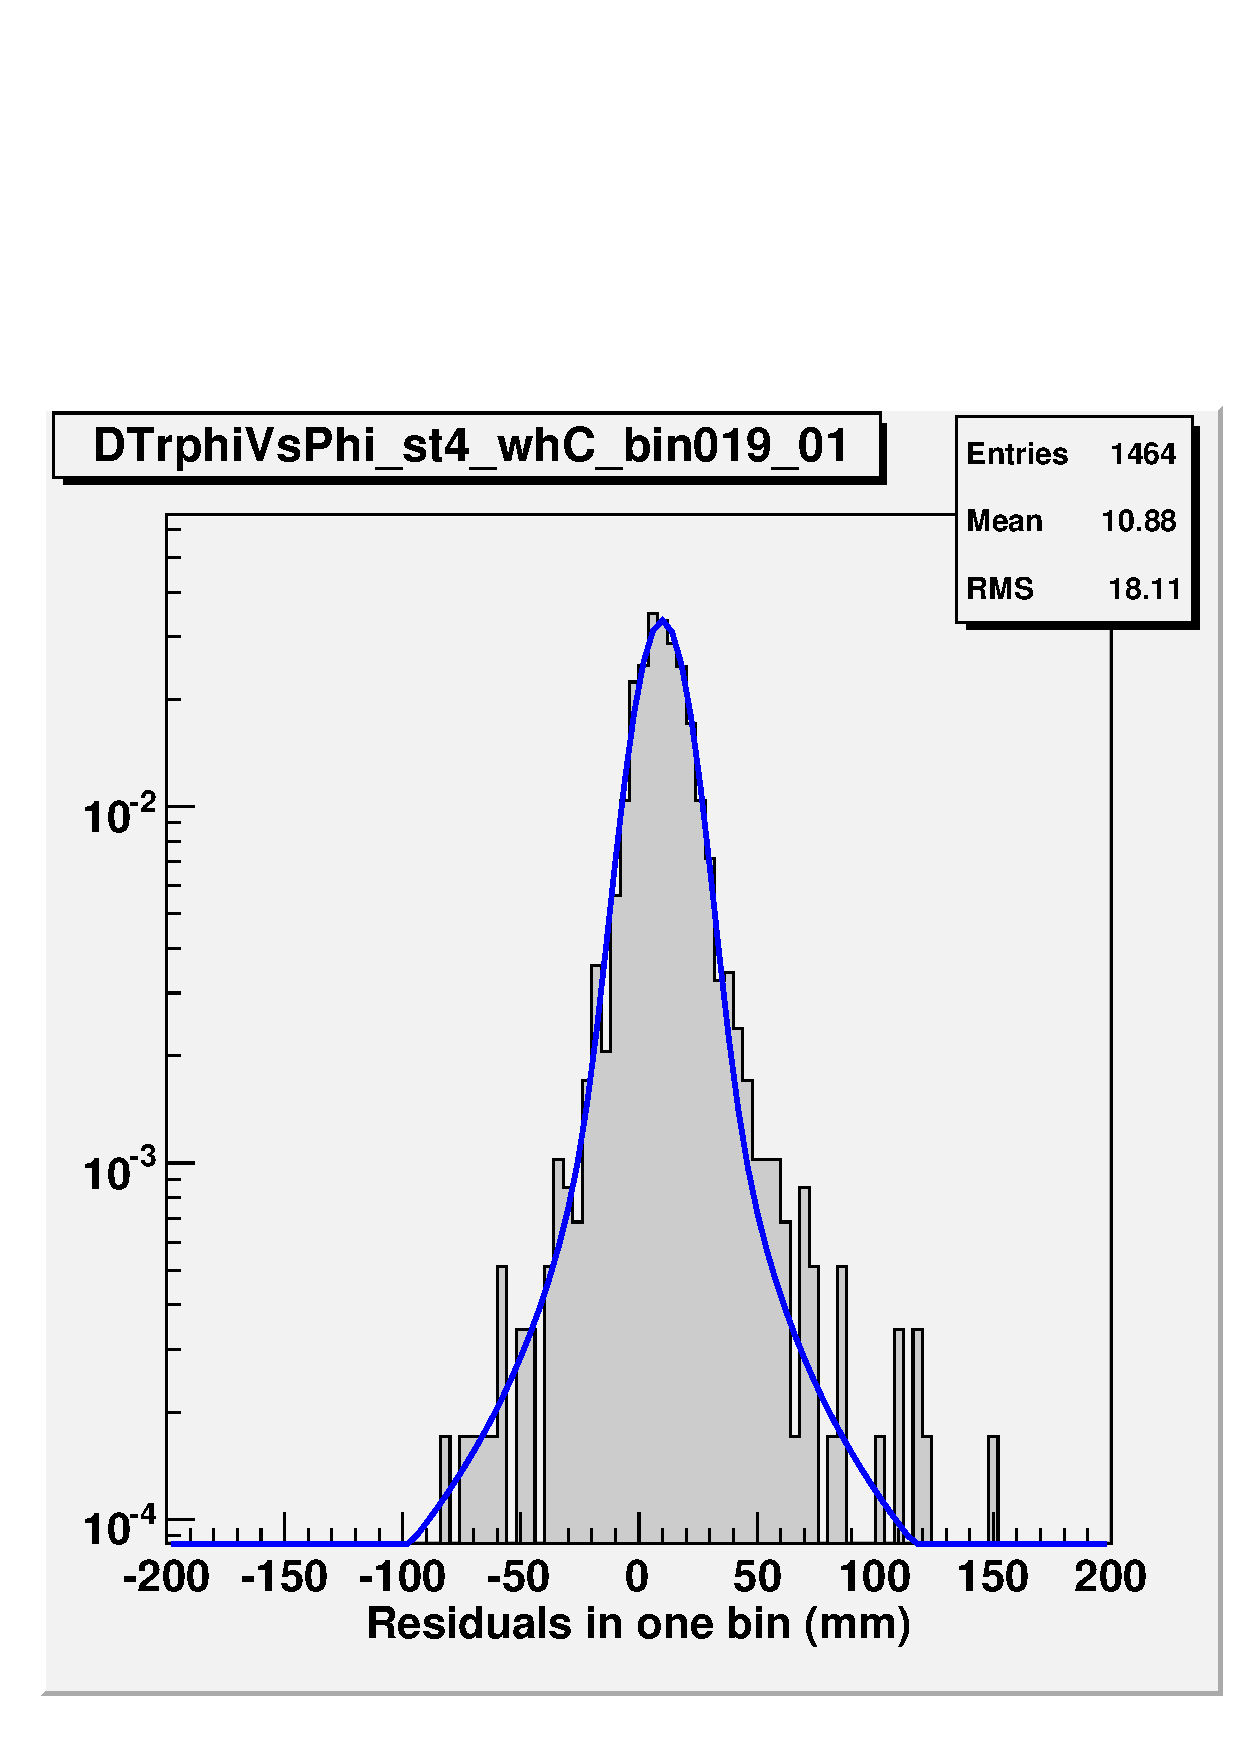
\includegraphics[width=\linewidth]{fitfunction.pdf}
\end{columns}

\begin{itemize}
\item Naturally has a Gaussian core, power-law tails, and is self-normalized
\item Models the physical process: scattering effects yield power-law
  distributions, experimental resolution adds Gaussian convolution
\item Unbinned fit acts like a mean that de-emphasizes outliers
\begin{itemize}
\item power-law contributes far less to log liklihood than exponential
\item regular mean ($\sum x_i/N$) would be equal to center of an unbinned Gaussian fit; this is a small extension, adding the tails
\end{itemize}
\end{itemize}
\end{frame}

%% what difference does it make? [plot]
%%    very similar to simple profile plots
%%    edges are sharper, plateaus are sharper
%%    -> confidence that what we're doing is rigorous

\begin{frame}
\frametitle{What difference does it make?}
\begin{itemize}
\item Similar to old profile plots (this is the ``twist'' plot from last time)
\item Small corrections compared to the effects we showed before
\item Added confidence that what we're doing is rigorous
\end{itemize}

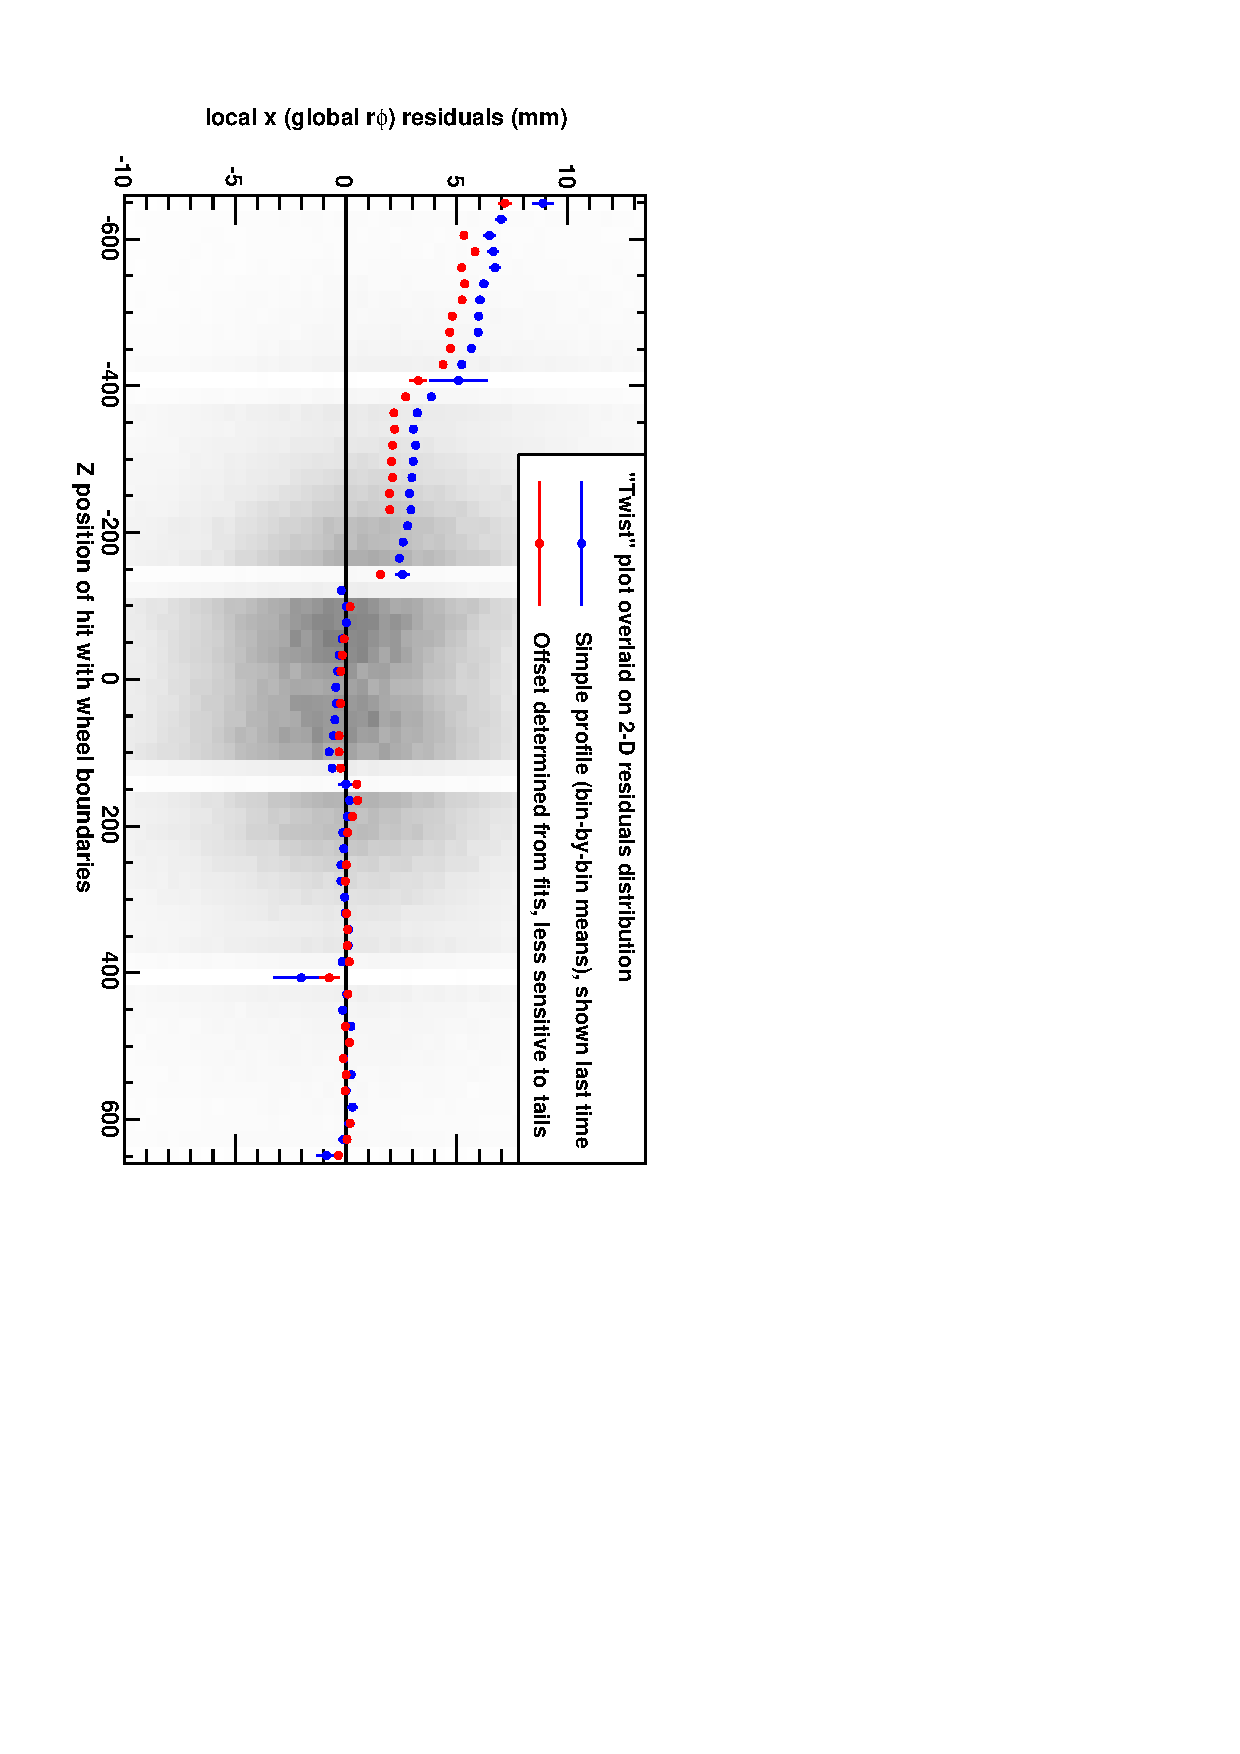
\includegraphics[height=\linewidth, angle=90]{twist_fit_demonstration.pdf}
\end{frame}

%% Cartography [plot: rphi vs z, station 2 sector 12]
%%    * I've split up the data such that we can now see individual
%%      chambers, rather than wheels, clearer pattern is emerging
%%    * all plots have the same features:
%%      * grey background is raw residuals distribution
%%      * red points are bin-by-bin fit results, averaging positive and
%%        negative track results to be insensitive to B field errors
%%      * small blue points are the difference, illustrating the B field
%%        error that would be incurred if we only used positive tracks
%%        (maximal)
%%    * plots vs z are split by sector, plots vs phi are split by wheel:
%%      you only see one chamber at a time

\begin{frame}
\frametitle{Cartography}
\begin{itemize}
\item I've split up the data so that we can see individual chambers
\begin{itemize}
\item plots vs.\ $z$ are split by sector, plots vs.\ $\phi$ are split
  by wheel: you only see one chamber at a time
\end{itemize}
\item All have the same features:
\begin{itemize}
\item grey background is raw 2-D residuals distribution
\item red points are bin-by-bin fit results, insensitive to
  $\vec{B}$-field mismodelling because of $+$/$-$ averaging procedure
\item small blue points are $+$/$-$ difference: the error we would
  incur if we were crazy enough to use only positive tracks (maximal)
\end{itemize}
\end{itemize}

\vspace{-0.4 cm}
\begin{center}
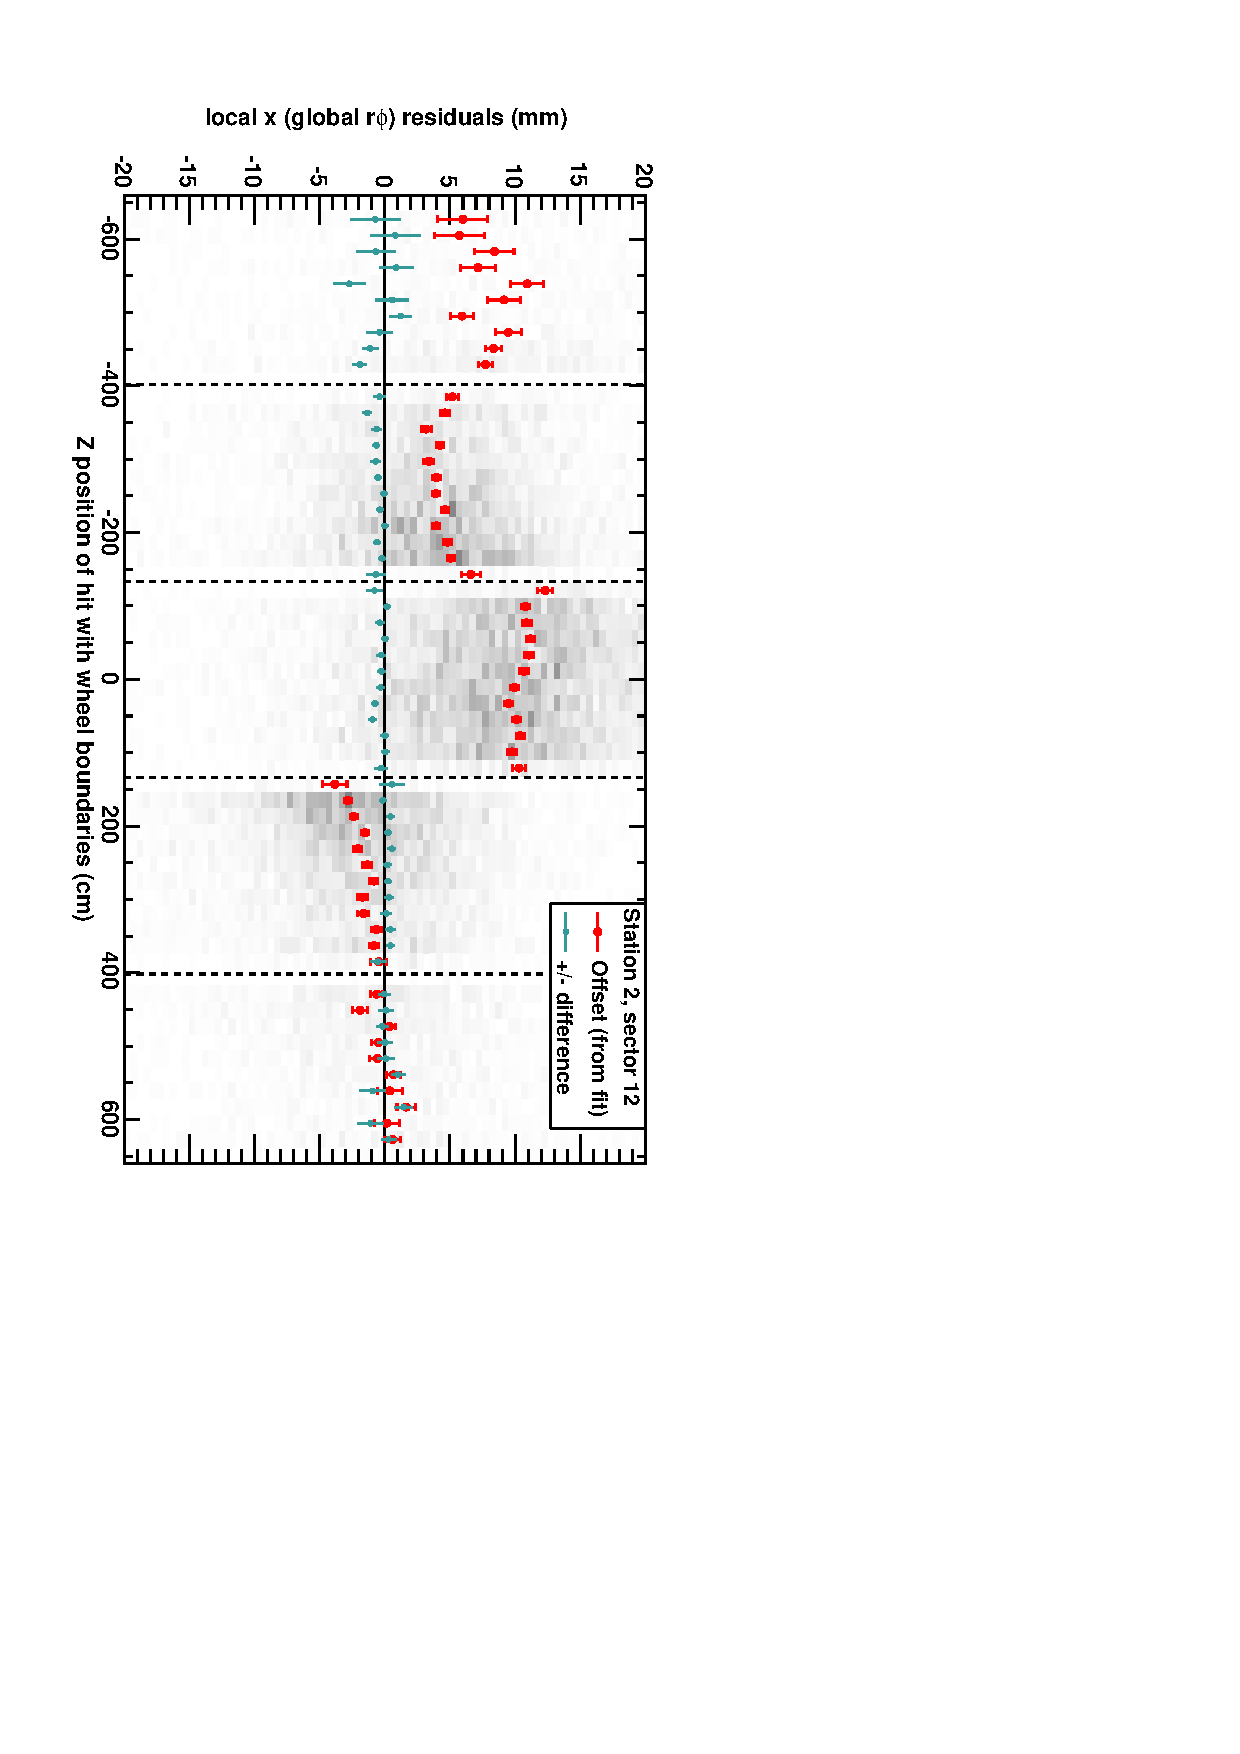
\includegraphics[height=0.75\linewidth, angle=90]{DTrphiVsZ_st2_sr12.pdf}
\end{center}
\end{frame}

%% Geography 1/4: cliffs [plot: rphi vs z, station 1 sector 8]
%%    * offsets in local x residuals from one chamber to the next are
%%      (rather large) rphi displacements
%%    * discontinuities in the curve are a smoking gun
%%    * linear slope with respect to z can be easily explained by phi_z
%%      rotations

\begin{frame}
\frametitle{Geography: local $x$ cliffs}
\begin{itemize}
\item Offsets in local $x$ residuals from one chamber to the next \\ are
  (rather large) $r\phi$ displacements
\begin{itemize}
\item discontinuities in the curve are a smoking gun!
\end{itemize}
\item Linear slopes with respect to $z$ can be easily explained \\ by local $\phi_z$ rotations
\end{itemize}

\begin{center}
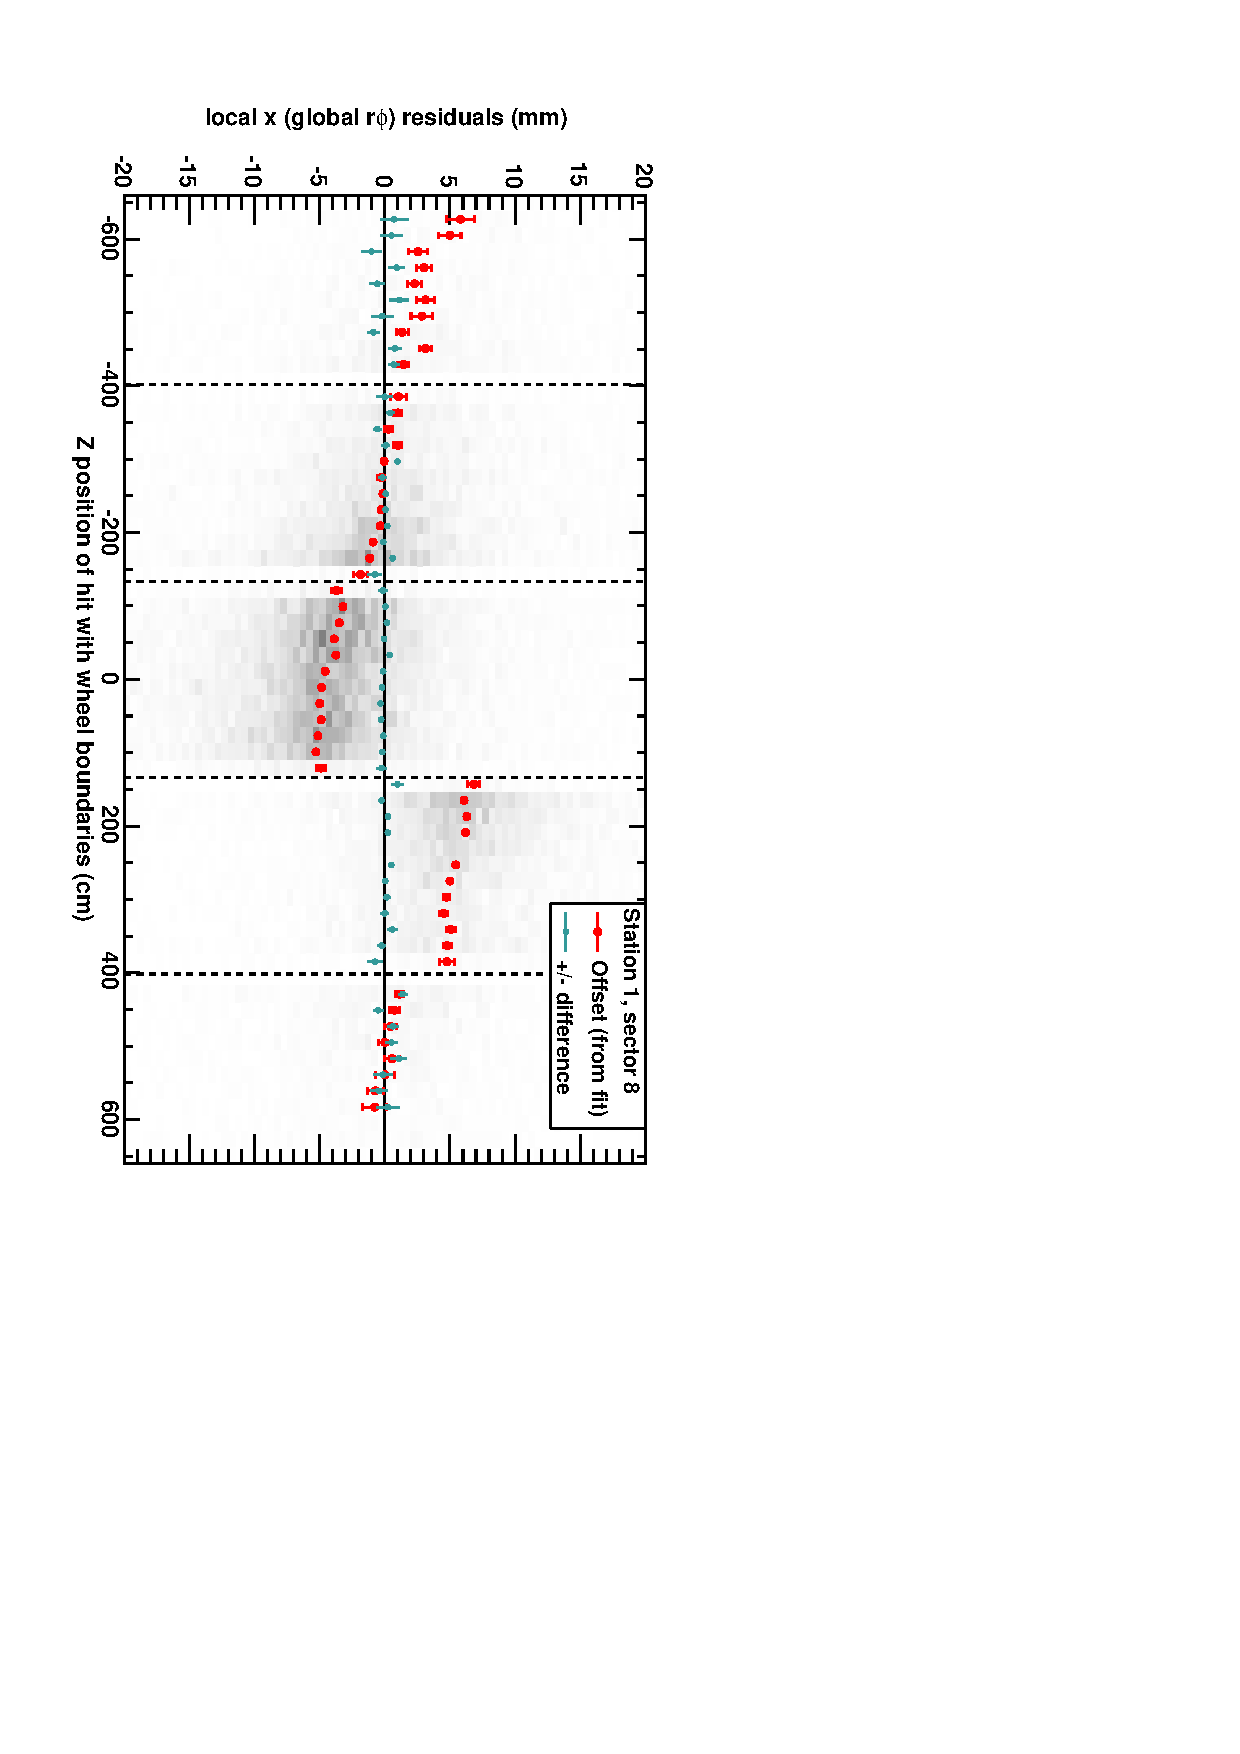
\includegraphics[height=\linewidth, angle=90]{DTrphiVsZ_st1_sr08.pdf}
\end{center}
\end{frame}

%% Geography 2/4: sawtooth mountains [plot rphi vs phi, station 1 wheel 1]
%%    * linear slopes in local x residuals vs. phi can be explained by
%%      - rather large radial displacements: DeltaR approx residual * (R/chamber half-length)
%%      - huge phi_y rotations: (Delta phi_y)^2 approx 1 - residual / chamber half-length
%%    * if one of these is responsible, it will become more clear in
%%      track-by-track calculation of DeltaR and Delta phi_y vs phi

\begin{frame}
\frametitle{Geography: sawtooth mountains}
\begin{itemize}
\item Linear slopes in local $x$ residuals vs.\ $\phi$ can be explained by
\begin{itemize}
\item rather large radial displacements: 

\mbox{ } \hfill $\Delta R \approx (\mbox{maximum residual}) \times (R/\mbox{chamber half-length})$ \hfill \mbox{ }

\item or huge local $\phi_y$ rotations: 

\mbox{ } \hfill $(\Delta \phi_y)^2 \approx 1 - (\mbox{maximum residual}) / (\mbox{chamber half-length})$ \hfill \mbox{ }

\end{itemize}
\item If one of these is responsible, it will become more clear in the track-by-track calculation of $\Delta R$ and $\Delta \phi_y$ \mbox{(I can also plot that vs.\ $\phi$)\hspace{-1 cm}}
\end{itemize}

\vspace{-0.4 cm}
\begin{center}
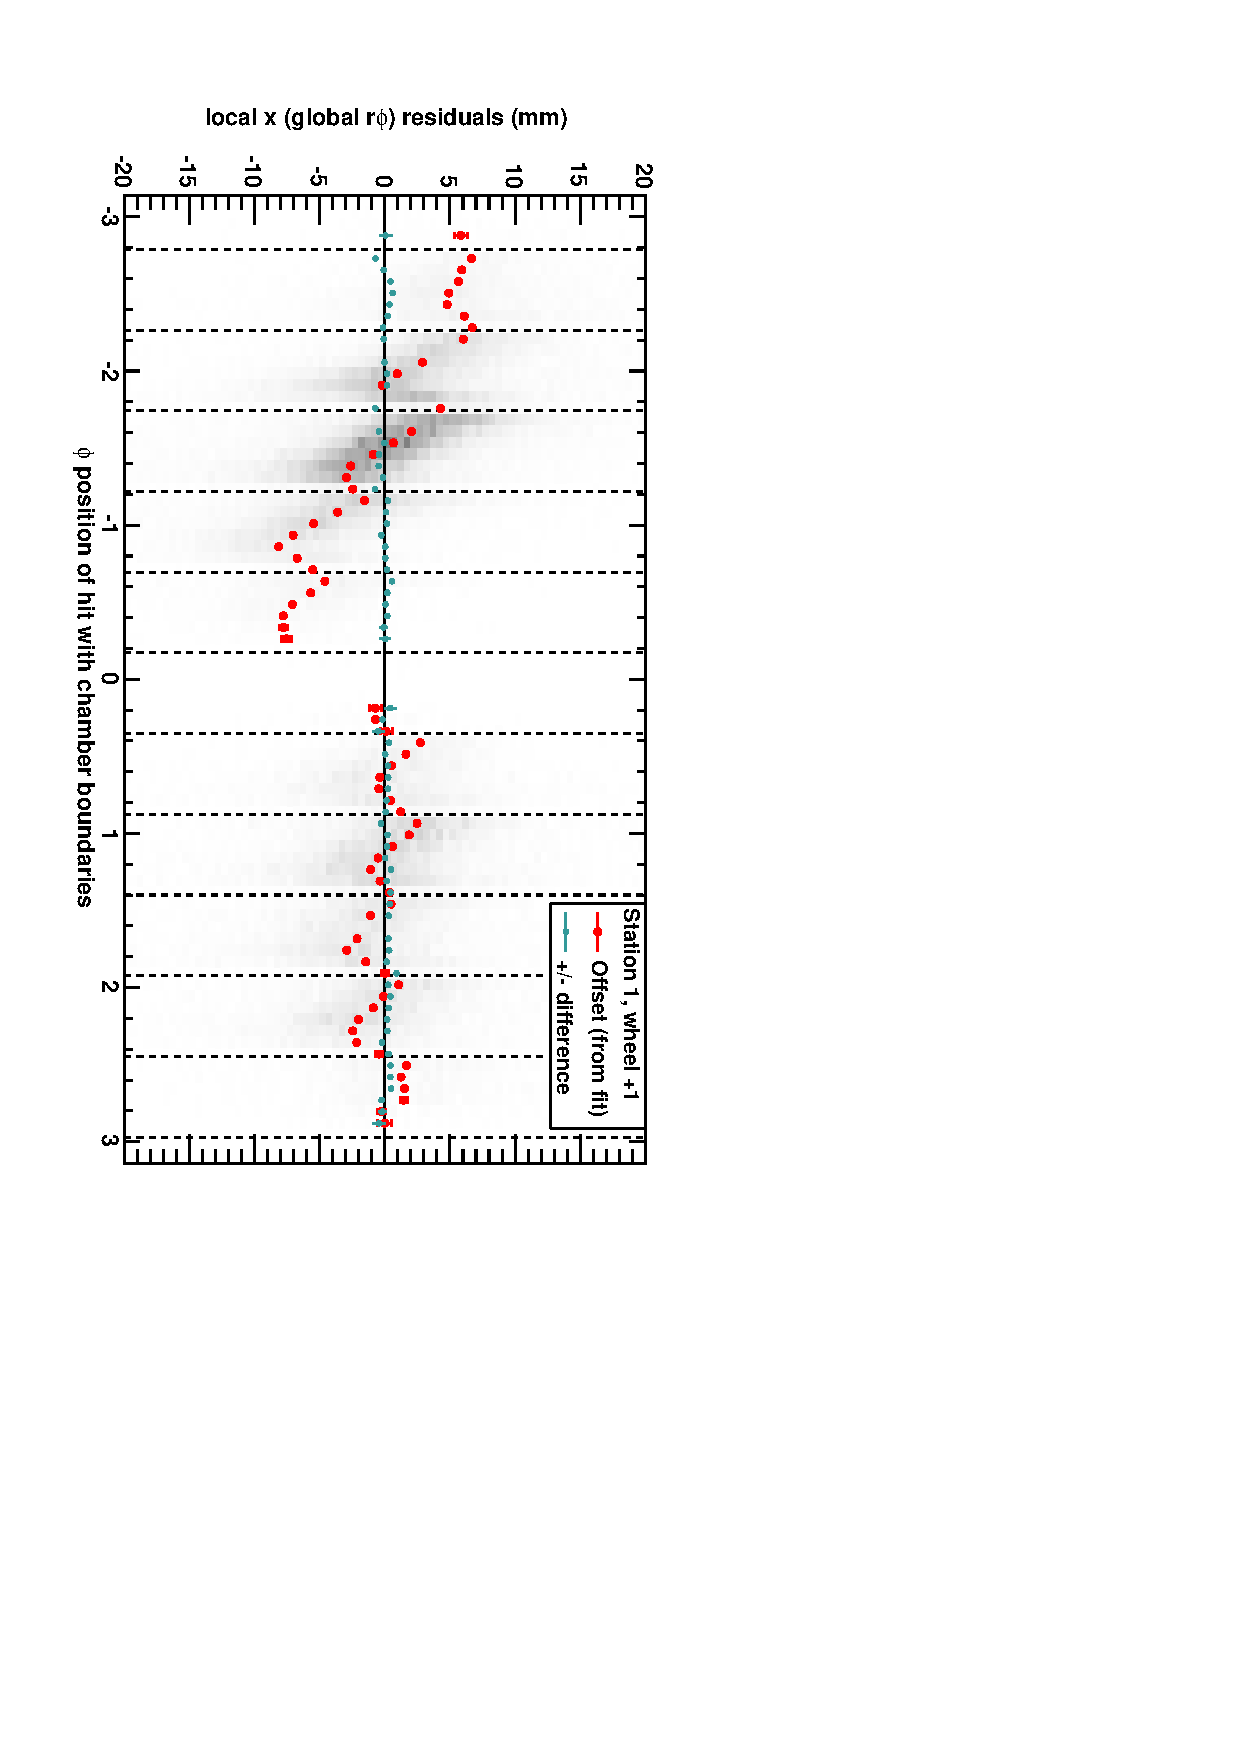
\includegraphics[height=0.9\linewidth, angle=90]{DTrphiVsPhi_st1_whD.pdf}
\end{center}
\end{frame}

%% Geography 3/4: B-field plateaus [plot rphidiff 3-2, wheel 0]
%%    * magnetic field errors (blue points) are visible in station 3
%%      and especially station 4
%%    * they can be localized by considering track-by-track differences
%%      in residuals on one station minus residuals on another station
%%      (here, station 3 minus station 2)
%%    * in wheel 0 only, they show a chamber-by-chamber dependence: a
%%      clue to the problem in field modelling?  (material between chambers?)

\begin{frame}
\frametitle{Geography: $\vec{B}$-field plateaus}
\begin{itemize}
\item $\vec{B}$-field mismodelling (blue points) is visible in \mbox{station 3 and especially 4\hspace{-1 cm}}
\item They can be better localized by considering track-by-track
  differences in station 3 residuals minus station 2 residuals \mbox{(for example)\hspace{-1 cm}}
\item In wheel~0 only, they show a chamber-by-chamber dependence: a
  clue to the problem in $\vec{B}$-field modelling?  \mbox{(material between chambers?)\hspace{-1 cm}}
\end{itemize}

\begin{center}
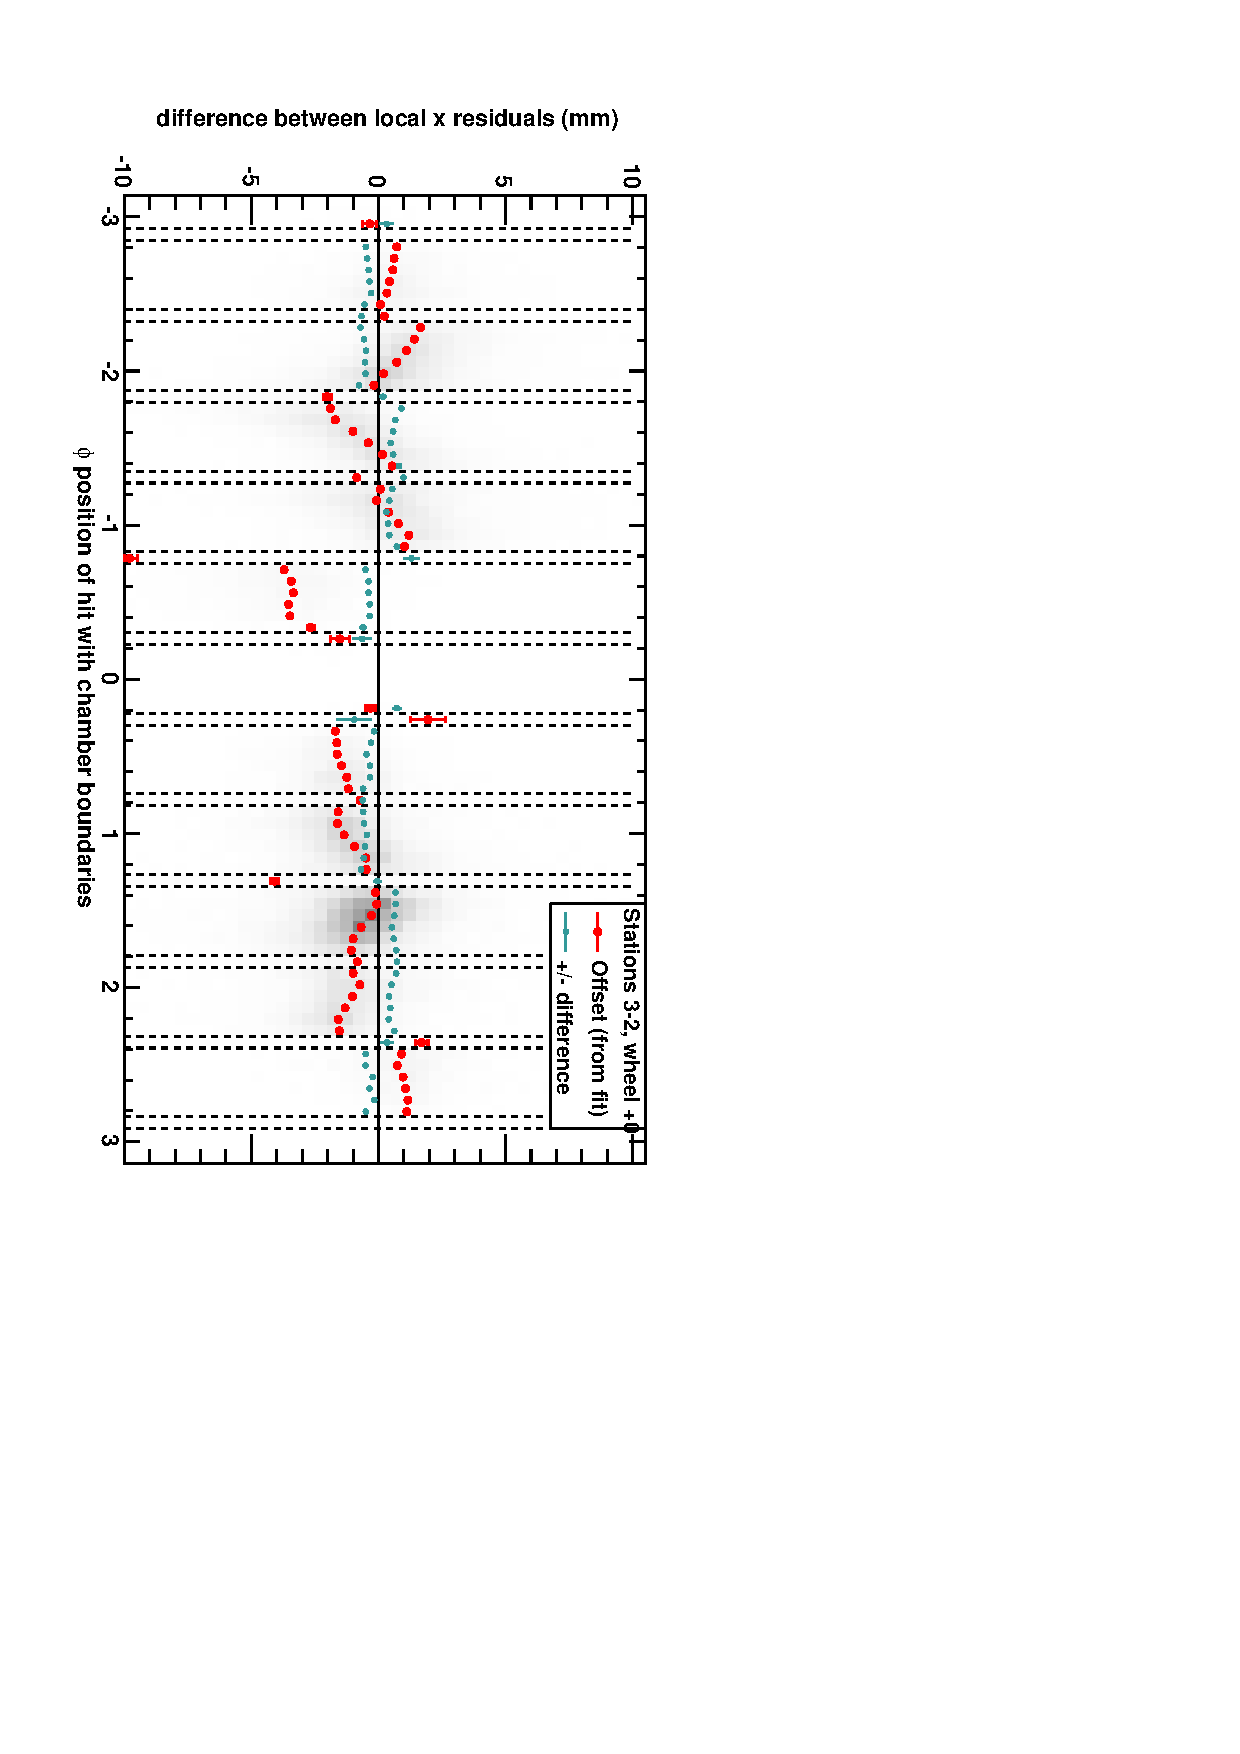
\includegraphics[height=\linewidth, angle=90]{DTrphidiff23VsPhi_whC_slope.pdf}
\end{center}
\end{frame}

%% Geography 4/4: smooth valleys [plot z vs phi, station 3 wheel 2]
%%    * local y residuals have a global trend with a maximum at phi = pm
%%      pi/2 and large |z|
%%    * appears in all stations, consistently in vs. phi and vs. z plots
%%    * though in principle this could be a systematic distortion of the
%%      muon system, we consider first the possibility that it is a
%%      tracking bias
%%    * could be due to tracker TEC misalignment (also misaligned
%%      parallel to the beamline, affecting large |z| the most)
%%    * easy check: drop tracks with TEC hits and replot

\begin{frame}
\frametitle{Geography: smooth valleys}
\begin{itemize}
\item Local $y$ residuals have a global trend with a maximum amplitude \\ at $\phi = \pm\pi/2$ and large $|z|$
\begin{itemize}
\item appears in all stations, consistently in ``vs.\ $\phi$'' and ``vs.\ $z$'' plots
\end{itemize}
\item Though in principle this could be a systematic distortion of the
  whole barrel, we first consider the possibility that it is a
  \mbox{tracking bias\hspace{-0.5 cm}}
\begin{itemize}
\item could be due to tracker TEC misalignment \\ \mbox{(also misaligned parallel to beamline, affecting large $|z|$ the most)\hspace{-1 cm}}
\item easy to check: drop tracks with TEC hits and replot
\end{itemize}
\end{itemize}

\vspace{-0.4 cm}
\begin{center}
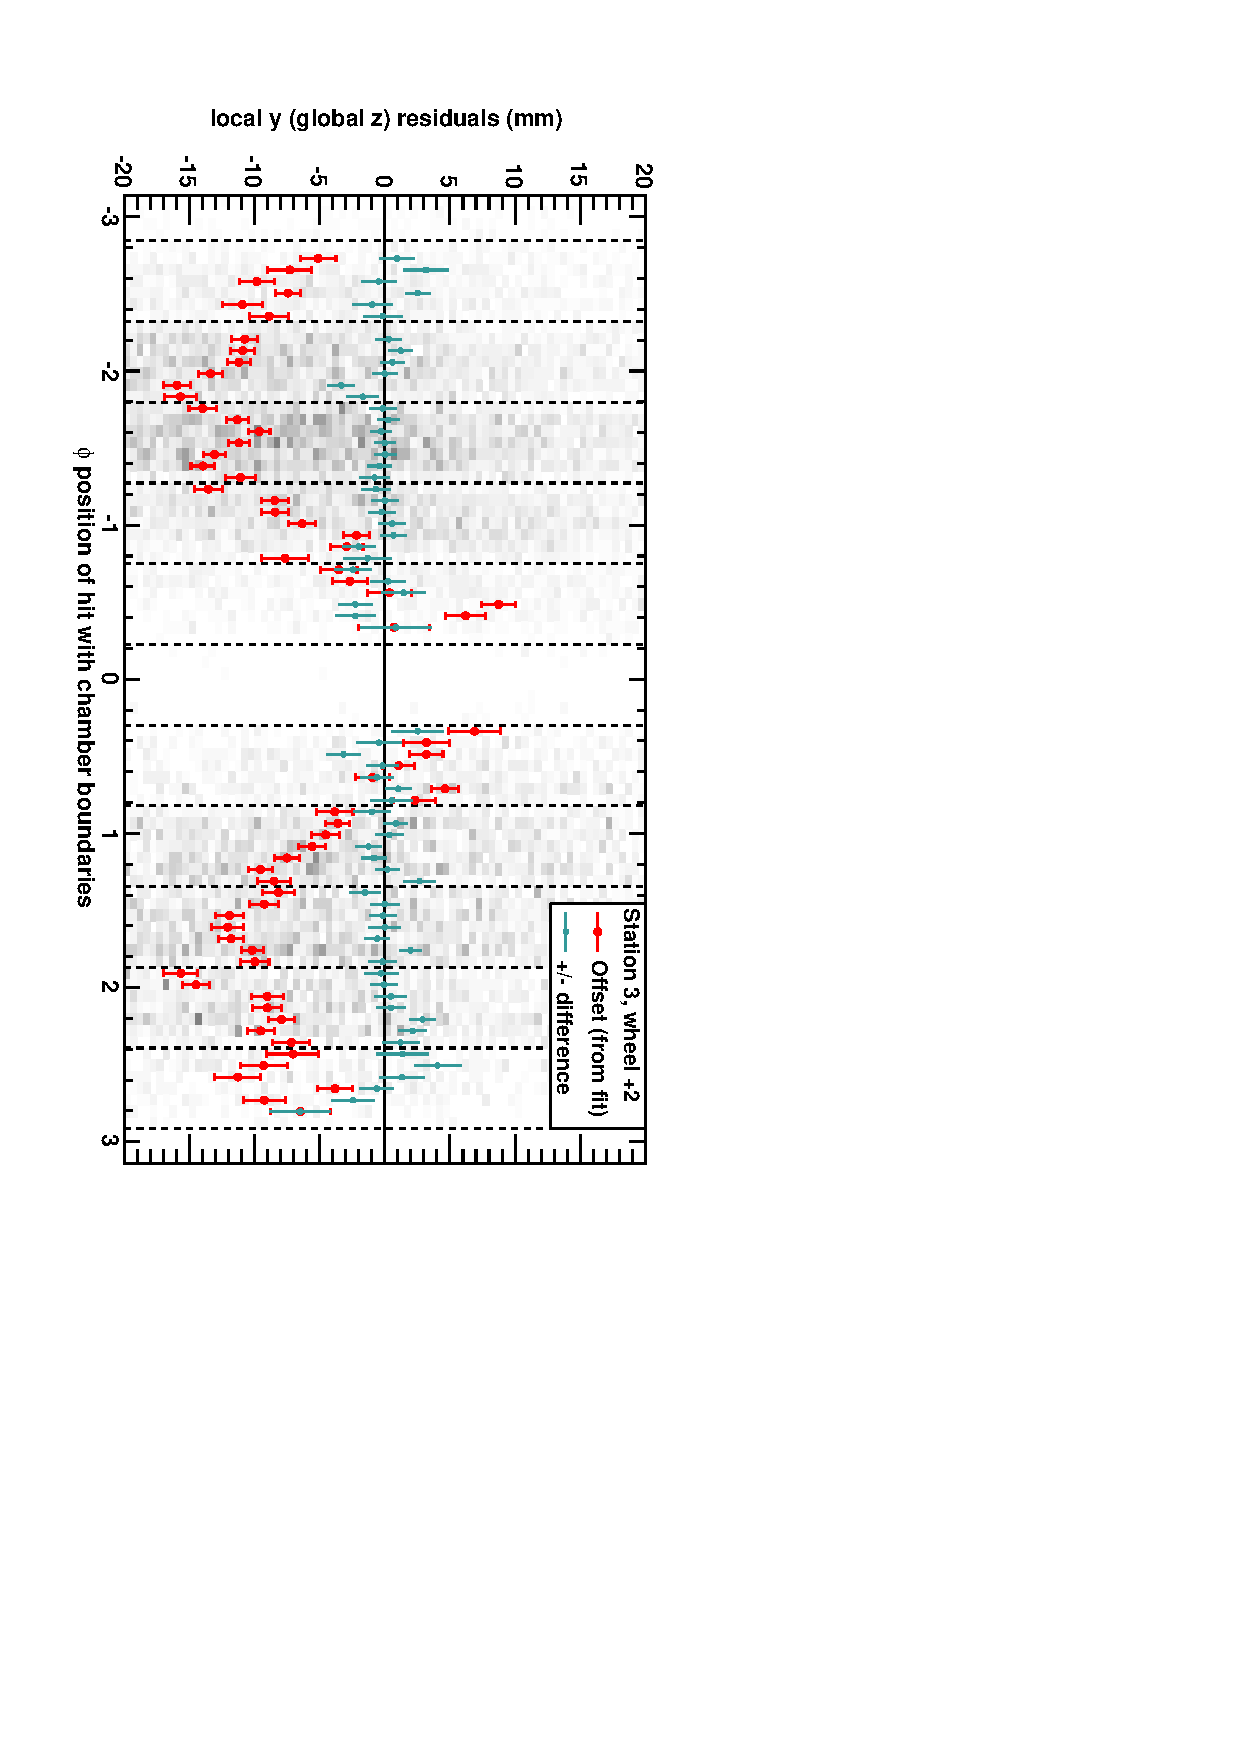
\includegraphics[height=0.83\linewidth, angle=90]{DTzVsPhi_st3_whE.pdf}
\end{center}
\end{frame}

%% Proposals for CRAFT
%%    minimal:
%%       incorporate improved fitting in alignment procedure and
%%       align local x (rphi) and phi_z (the plots present a clear
%%       picture that these are currently misaligned)
%%    more ambitious 1:
%%       make these kinds of plots for track-by-track DeltaR and Delta
%%       phi_y vs phi/z; if one of these is confirmed as being
%%       responsible for the ``sawtooth,'' apply corrections
%%    more ambitious 2:
%%       exclude tracks with TEC hits; if ``smooth valleys'' disappear,
%%       leaving only local y-residual cliffs, align local y
%%    combine with anything better measured by hardware, of course
%%       (through DTAlignmentRcd format)
%%    super-ambitious: align CSCs as well, but I don't think I have the time

\begin{frame}
\frametitle{Conclusion: CRAFT proposals}
\begin{itemize}
\item Minimal:
\begin{itemize}
\item incorporate improved fitting in alignment procedure
\item align local $x$ ($r\phi$) and local $\phi_z$ \\
\item the plots present a clear picture of their \mbox{current misalignment\hspace{-1 cm}}
\end{itemize}

\item More ambitious 1:
\begin{itemize}
\item make these kinds of plots for track-by-track $\Delta R$ and
  $\Delta \phi_y$
\item if one of these parameters is confirmed as being responsible for the ``sawtooth,'' apply corrections
\end{itemize}

\item More ambitious 2:
\begin{itemize}
\item exclude tracks with TEC hits
\item if ``smooth valleys'' disappear, leaving only local $y$ cliffs, align local $y$ (an important parameter)
\end{itemize}

\item Combine with anything better measured by hardware, of course \\
(through the DTAlignmentRcd format as input to track-based)

\item Too ambitious: aligning CSCs as well.  I don't think I have \mbox{enough time\ldots\hspace{-1 cm}}
\end{itemize}
\label{numpages}
\end{frame}

%% \begin{frame}
%% \frametitle{Next steps (regardless of CRAFT)}
%% \begin{itemize}
%% \item Improvements to these plots
%% \begin{itemize}
%% \item compute ``local $z$ residuals,'' ``$\phi_y$ residuals'' and the rest
%% \item reject tracks with TEC hits
%% \end{itemize}
%% \item Produce barrel alignment described below
%% \item Reproduce tracker radiography plots with aligned DTs
%% \item Use new StandAloneCosmicMuon refitter to
%% \begin{itemize}
%% \item verify DT alignment from globalCosmicMuons
%% \item align the CSCs (and poorly-illuminated DTs) relative \mbox{to the barrel\hspace{-1 cm}}
%% \end{itemize}
%% \end{itemize}

%% \vspace{0.1 cm}
%% \hspace{-0.83 cm} \textcolor{darkblue}{\Large Proposal for CRAFT}

%% \vspace{0.05 cm}
%% \begin{itemize}
%% \item Align the following parameters for well-illuminated DTs:
%% \begin{itemize}
%% \item local $x$ {\scriptsize (clear discontinuities between chambers in $r_x$ vs.\ $\phi$)}
%% \item $\phi_z$ {\scriptsize (clear linear slopes within chambers in $r_x$ vs.\ $z$)}
%% \item \textcolor{darkblue}{\it if} local $z$ or $\phi_y$ is responsible for the linear slopes
%%   within chambers in $r_x$ vs.\ $\phi$, align it
%% \item \textcolor{darkblue}{\it if} excluding TEC hits removes the
%%   CMS-wide $r_z$ arcs, align local $y$ {\scriptsize (clear discontinuities on chamber boundaries in $r_z$)}
%% \end{itemize}
%% \end{itemize}

%% \end{frame}

\section*{Rphi residuals versus phi}
\begin{frame}
\begin{center}
  \Huge \textcolor{blue}{$r\phi$ residuals versus $\phi$}
\end{center}
\end{frame}

\section*{station 1, wheel -2}
\begin{frame} \vfill \mbox{\hspace{-1 cm}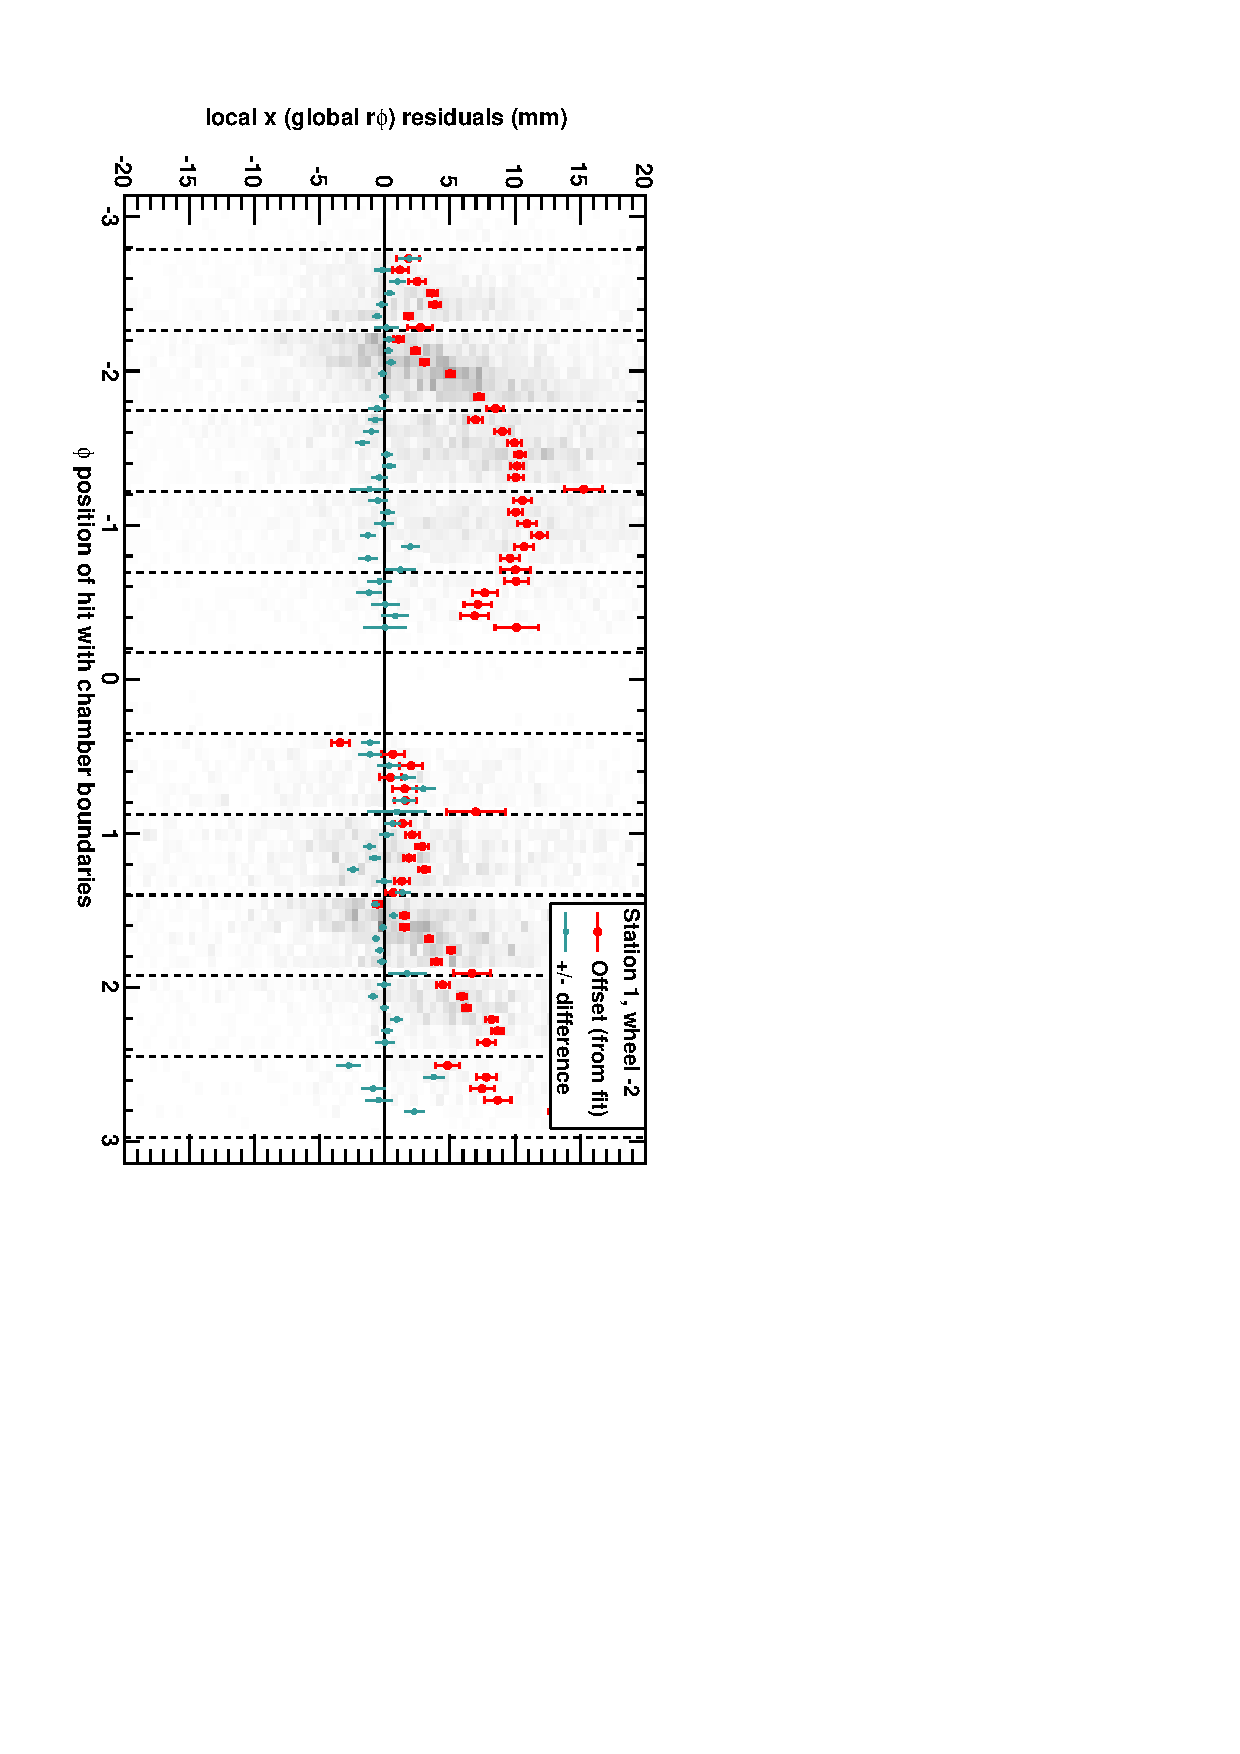
\includegraphics[height=1.2\linewidth, angle=90]{DTrphiVsPhi_st1_whA.pdf}} \end{frame}
\section*{station 1, wheel -1}
\begin{frame} \vfill \mbox{\hspace{-1 cm}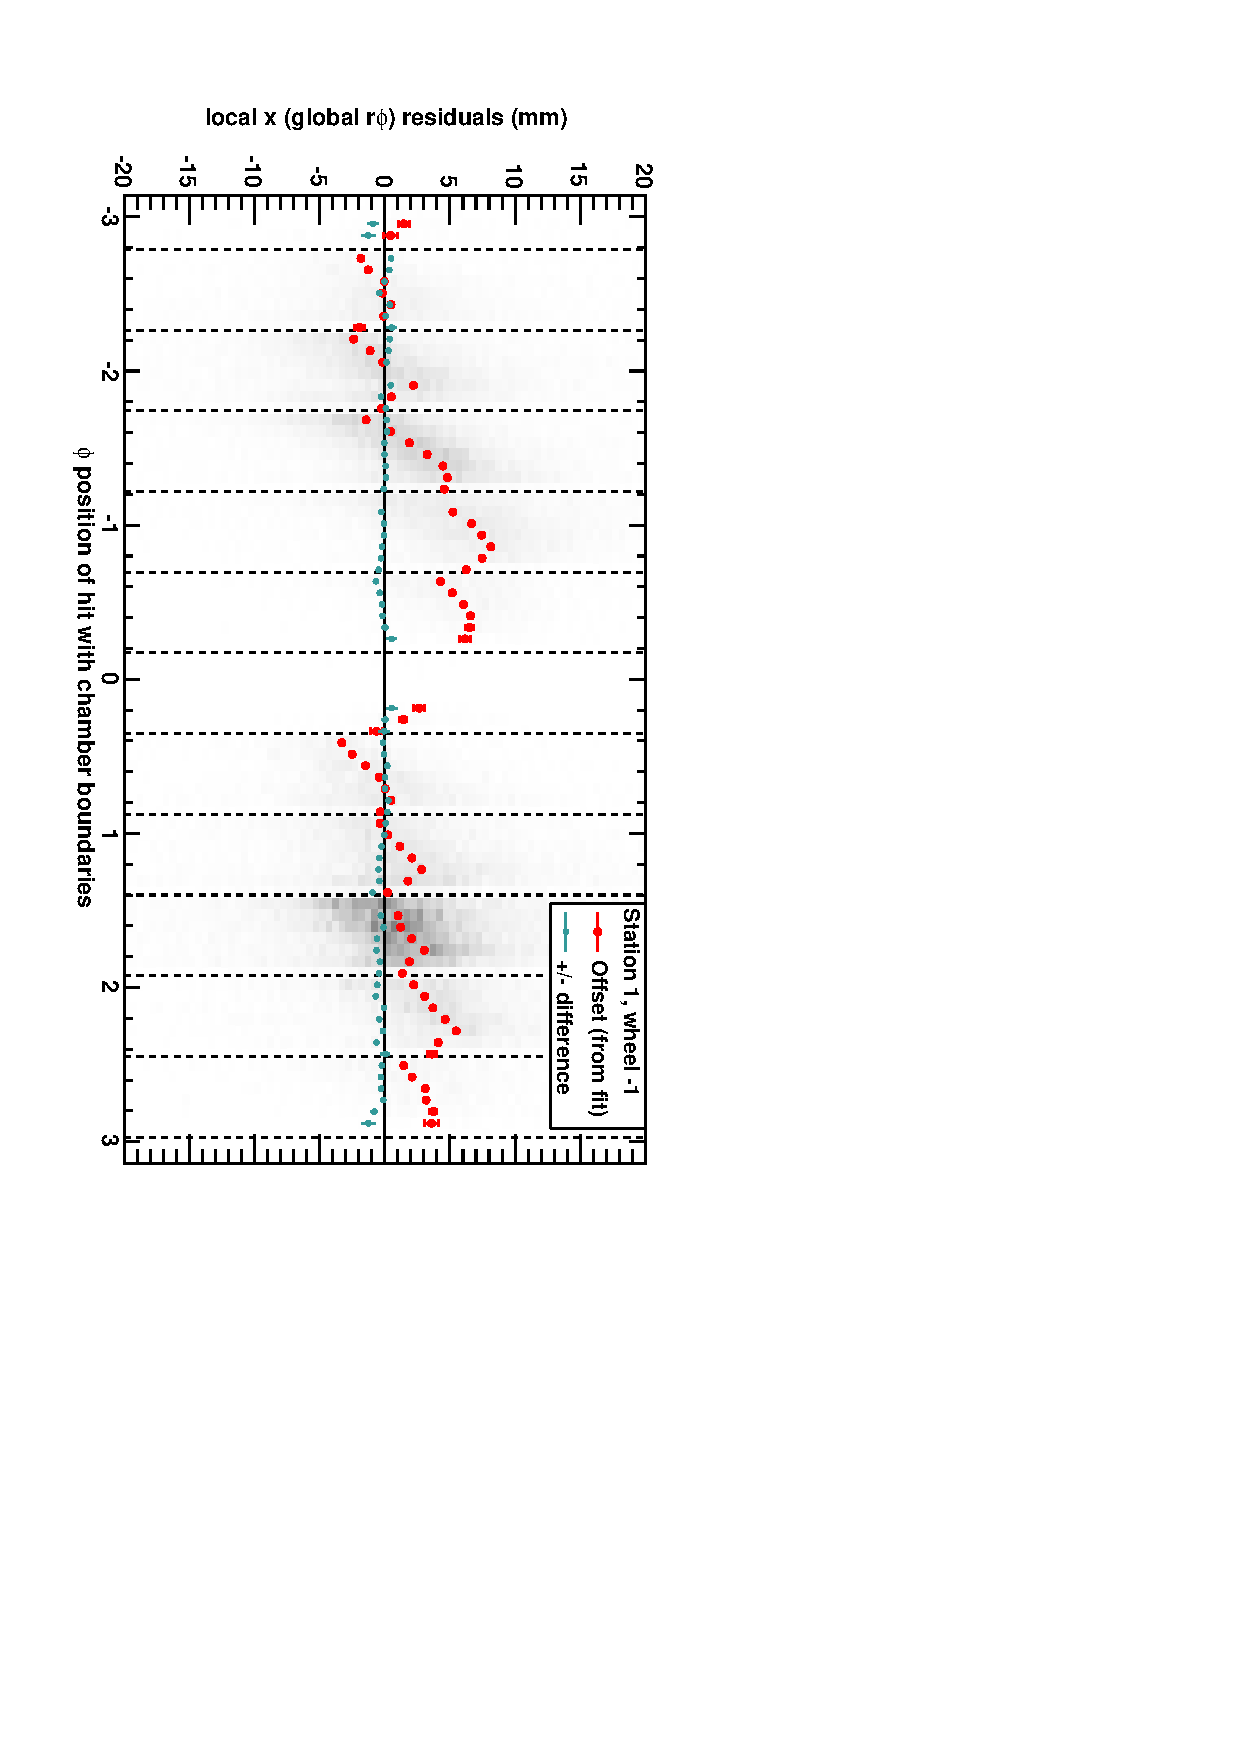
\includegraphics[height=1.2\linewidth, angle=90]{DTrphiVsPhi_st1_whB.pdf}} \end{frame}
\section*{station 1, wheel 0}
\begin{frame} \vfill \mbox{\hspace{-1 cm}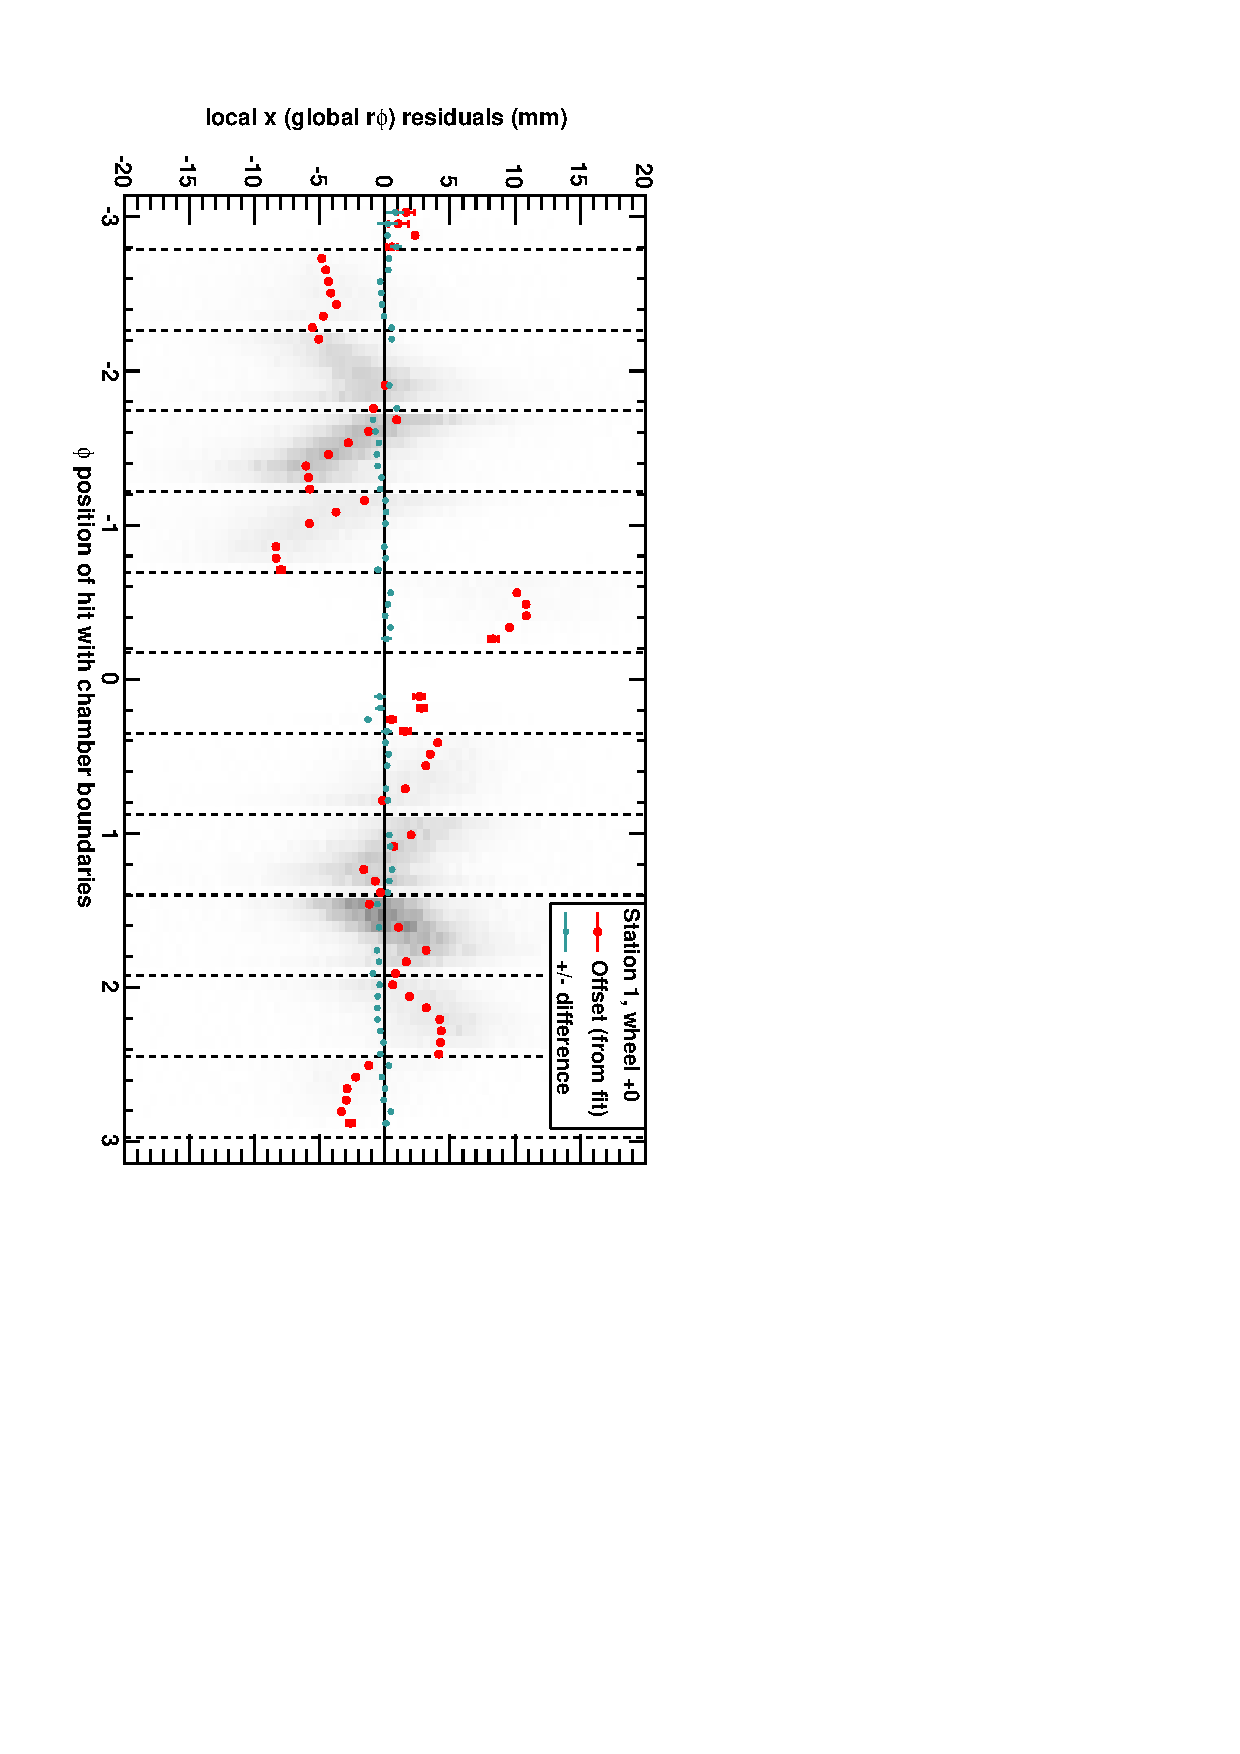
\includegraphics[height=1.2\linewidth, angle=90]{DTrphiVsPhi_st1_whC.pdf}} \end{frame}
\section*{station 1, wheel +1}
\begin{frame} \vfill \mbox{\hspace{-1 cm}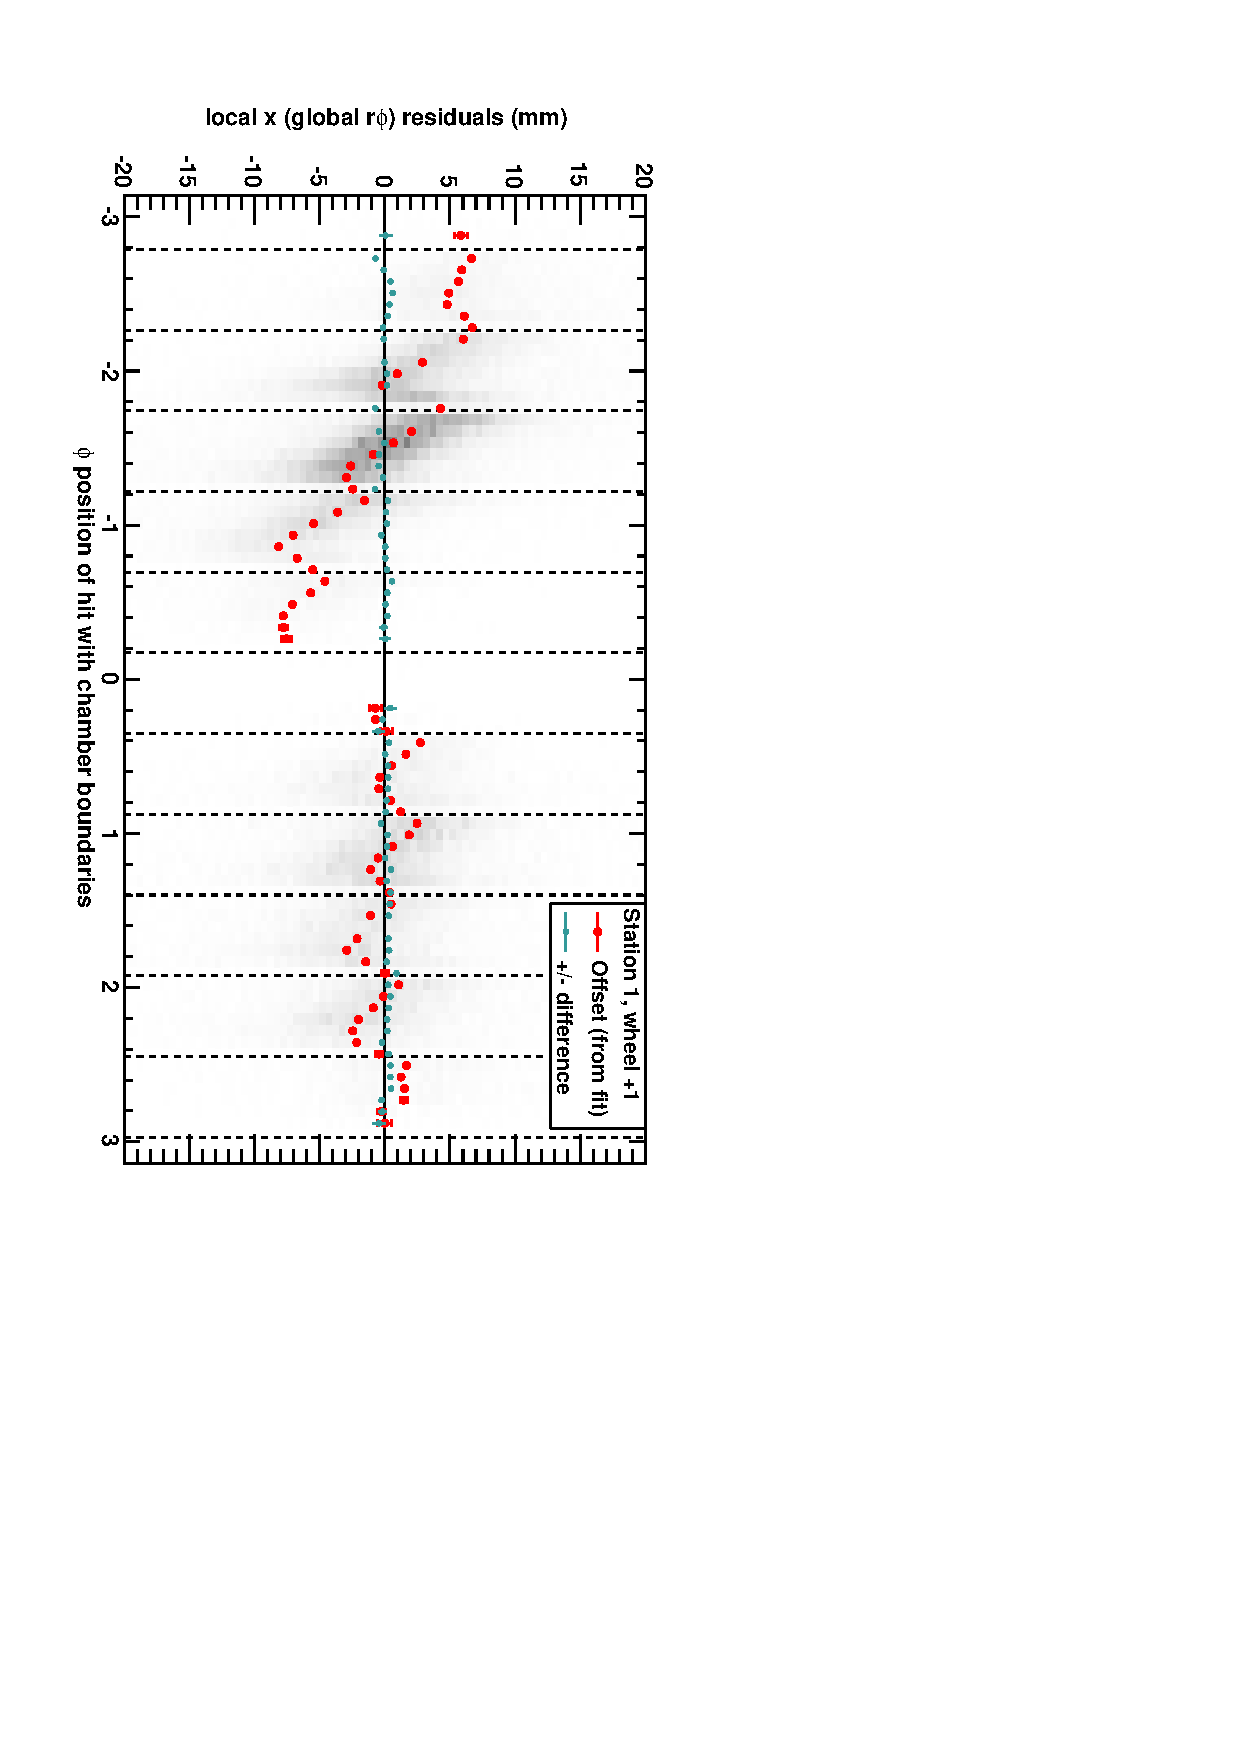
\includegraphics[height=1.2\linewidth, angle=90]{DTrphiVsPhi_st1_whD.pdf}} \end{frame}
\section*{station 1, wheel +2}
\begin{frame} \vfill \mbox{\hspace{-1 cm}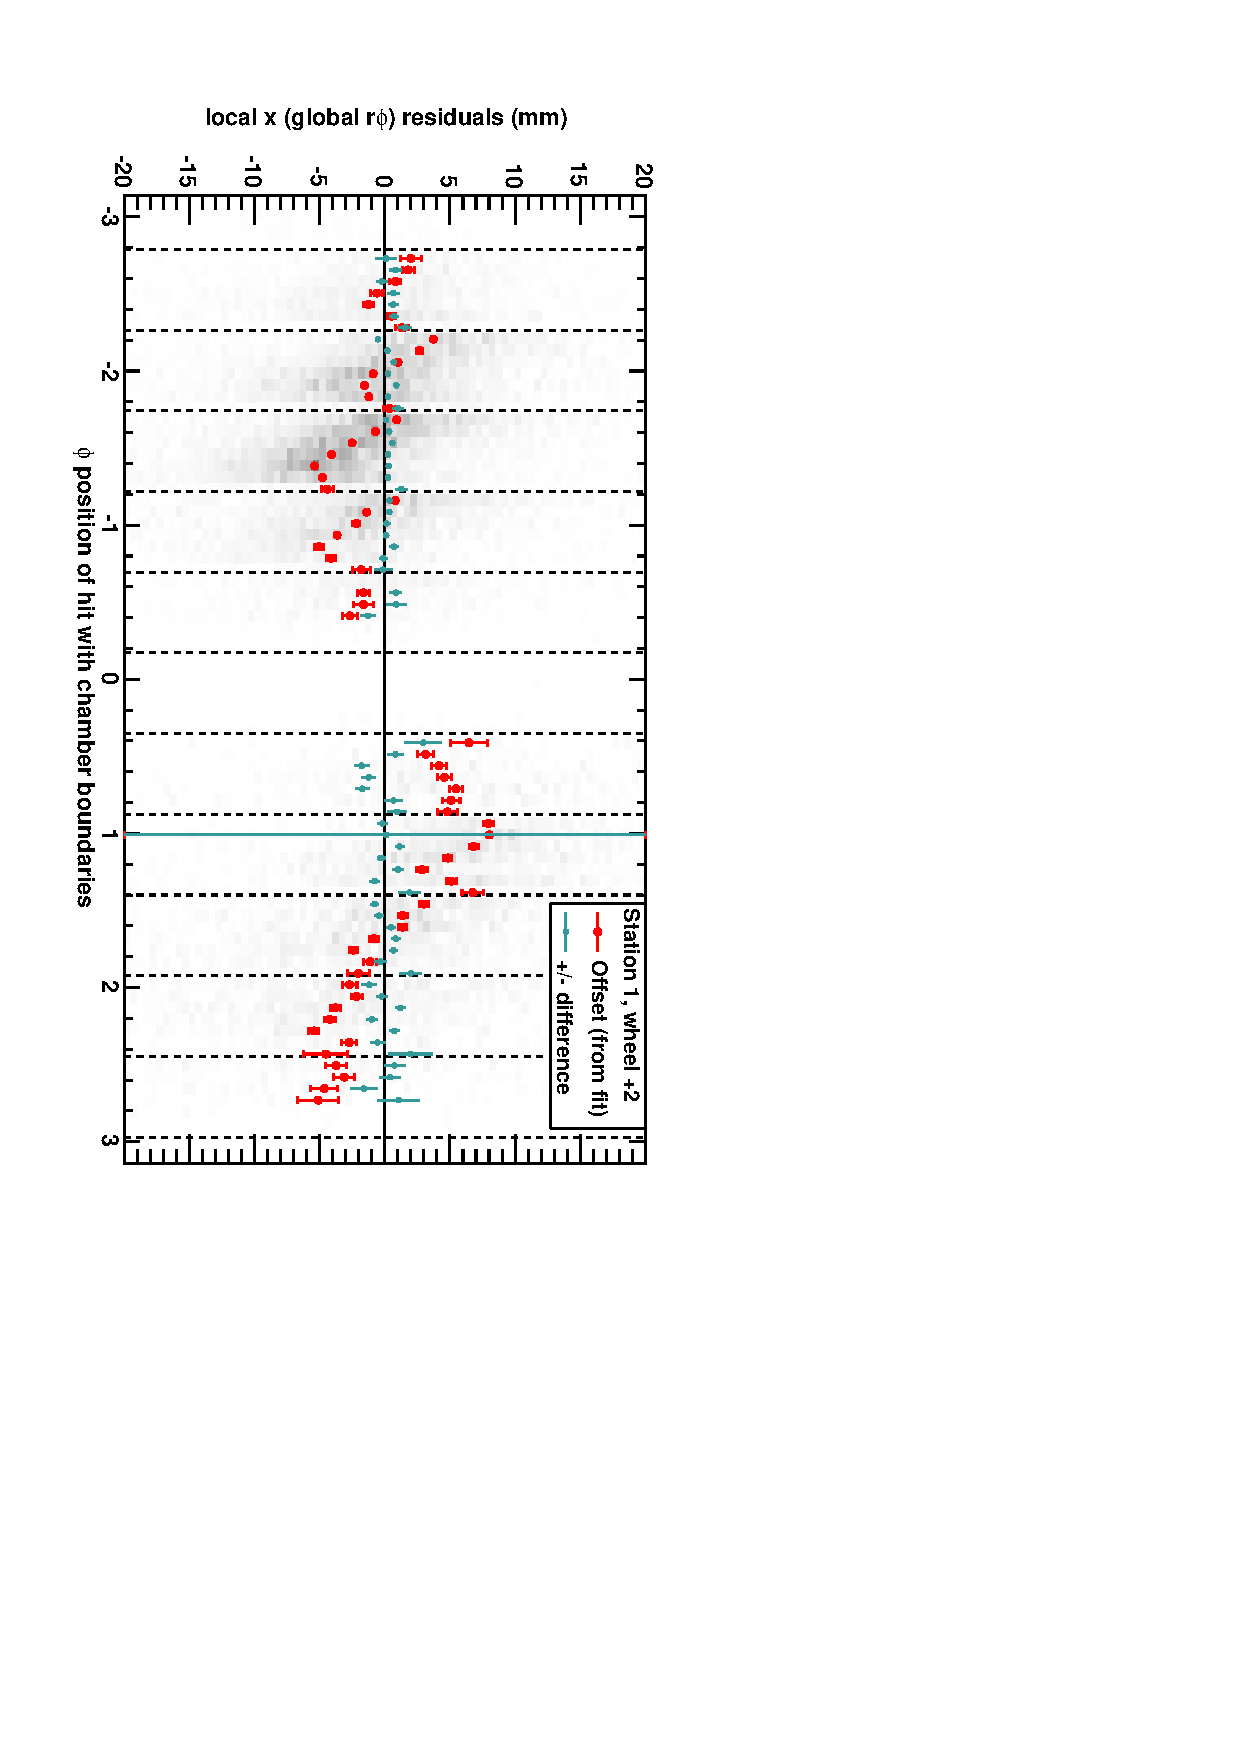
\includegraphics[height=1.2\linewidth, angle=90]{DTrphiVsPhi_st1_whE.pdf}} \end{frame}
\section*{station 2, wheel -2}
\begin{frame} \vfill \mbox{\hspace{-1 cm}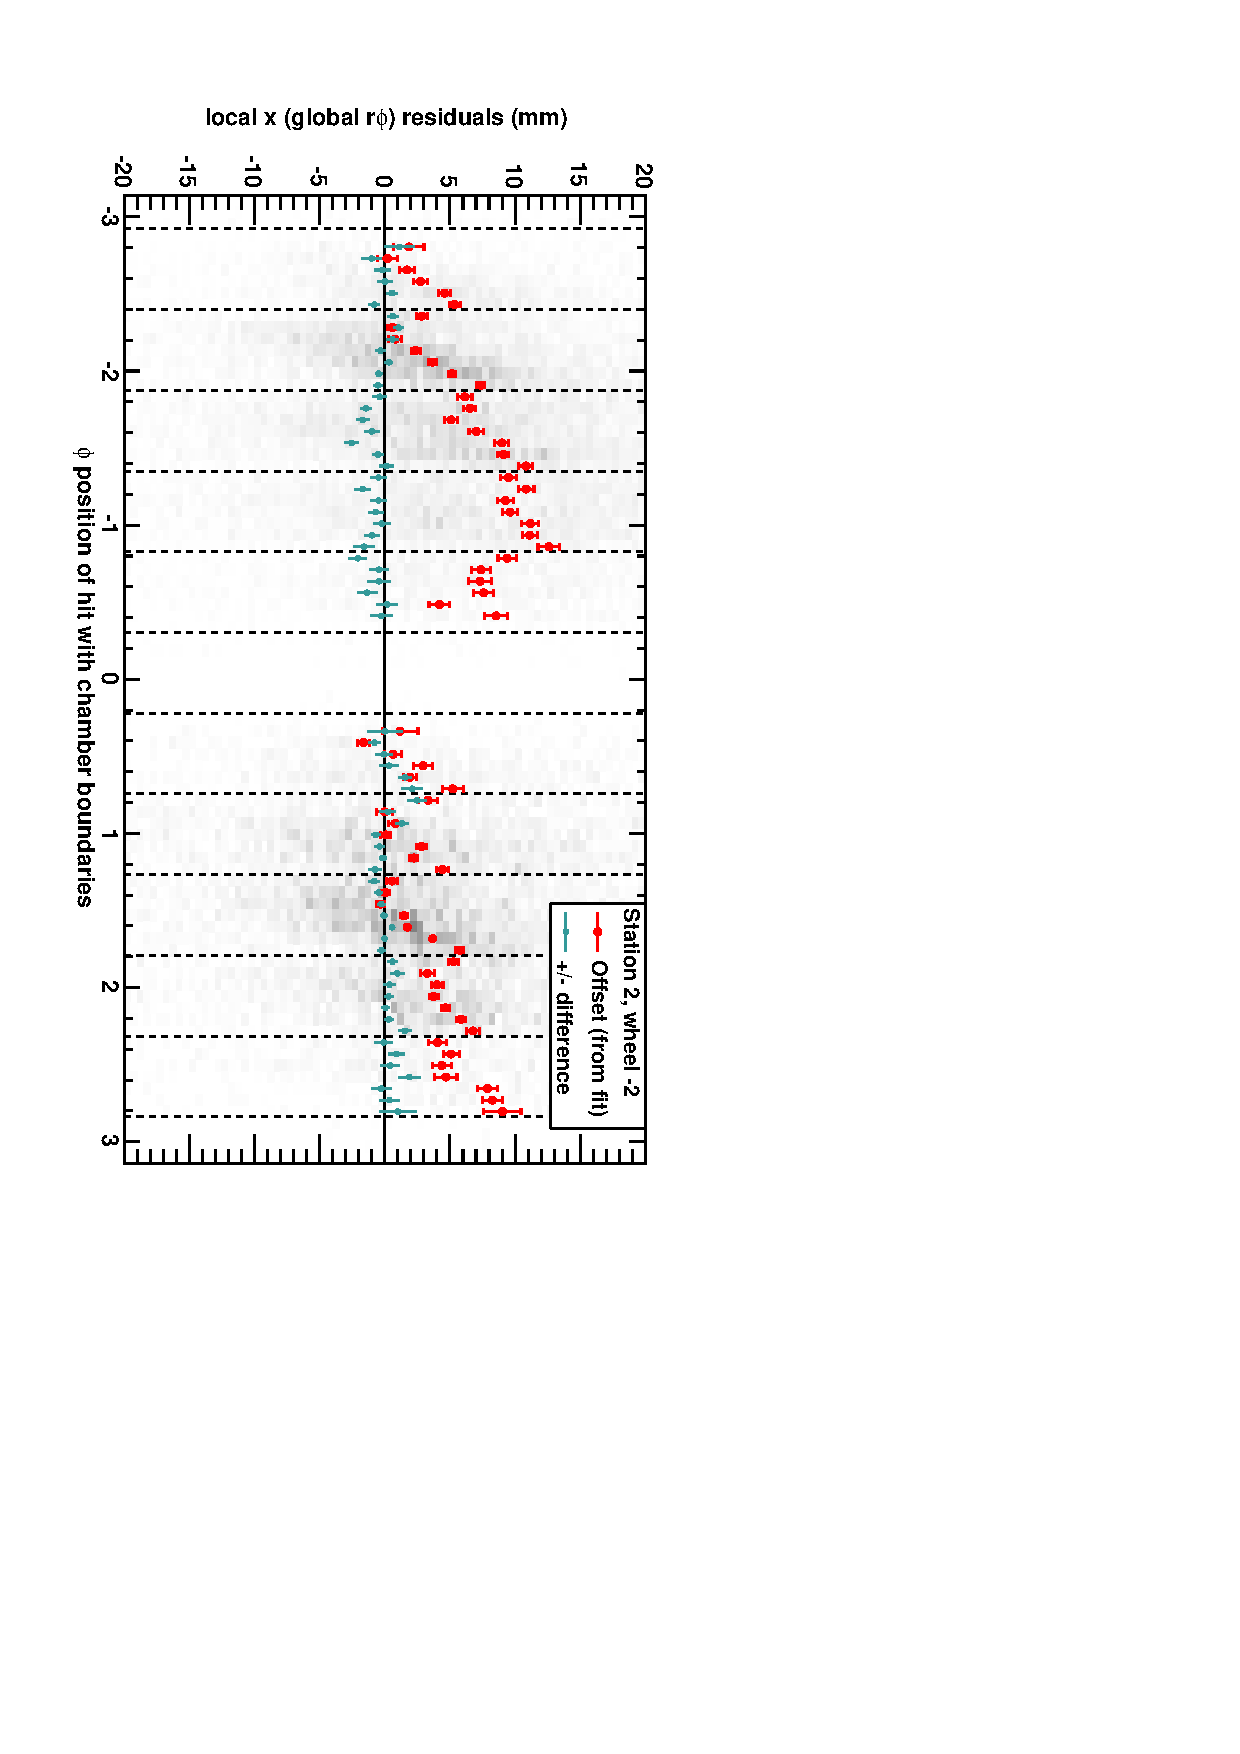
\includegraphics[height=1.2\linewidth, angle=90]{DTrphiVsPhi_st2_whA.pdf}} \end{frame}
\section*{station 2, wheel -1}
\begin{frame} \vfill \mbox{\hspace{-1 cm}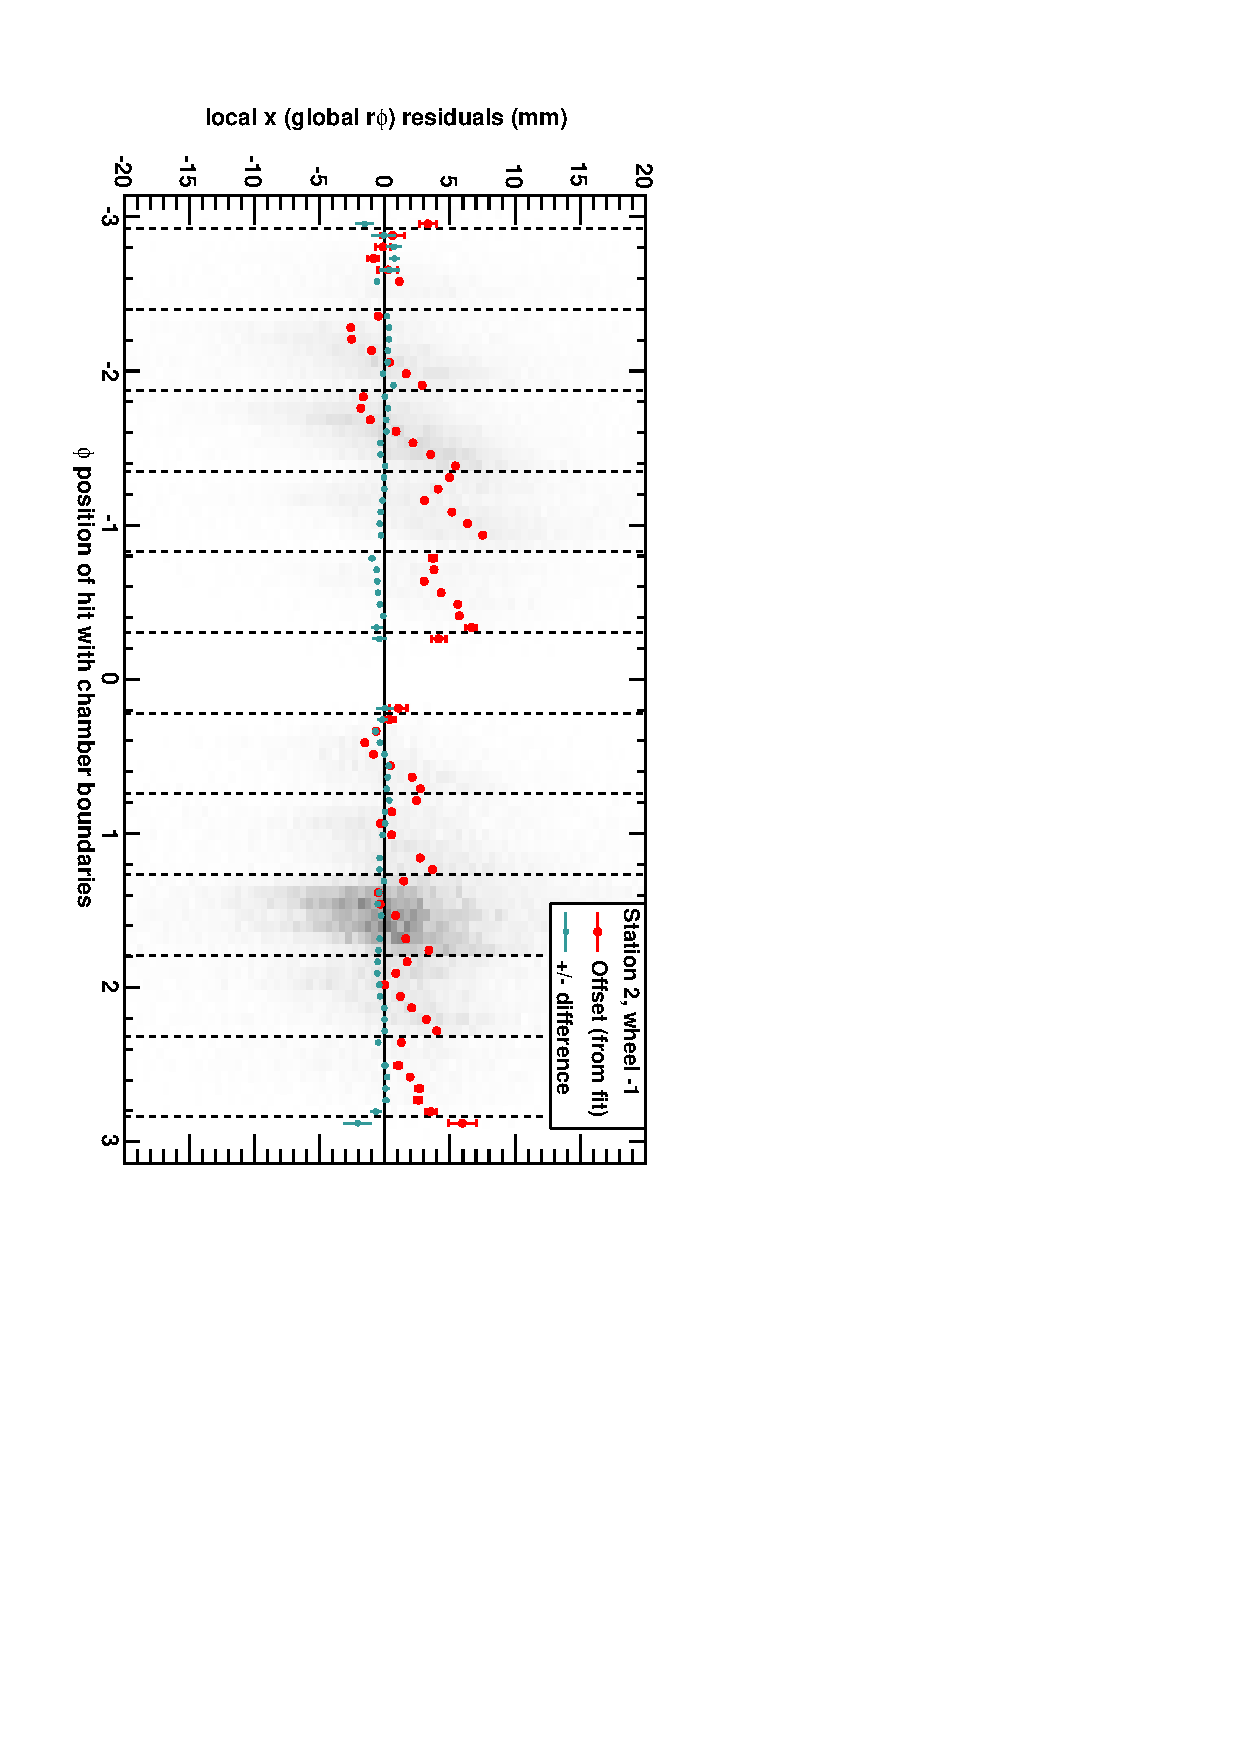
\includegraphics[height=1.2\linewidth, angle=90]{DTrphiVsPhi_st2_whB.pdf}} \end{frame}
\section*{station 2, wheel 0}
\begin{frame} \vfill \mbox{\hspace{-1 cm}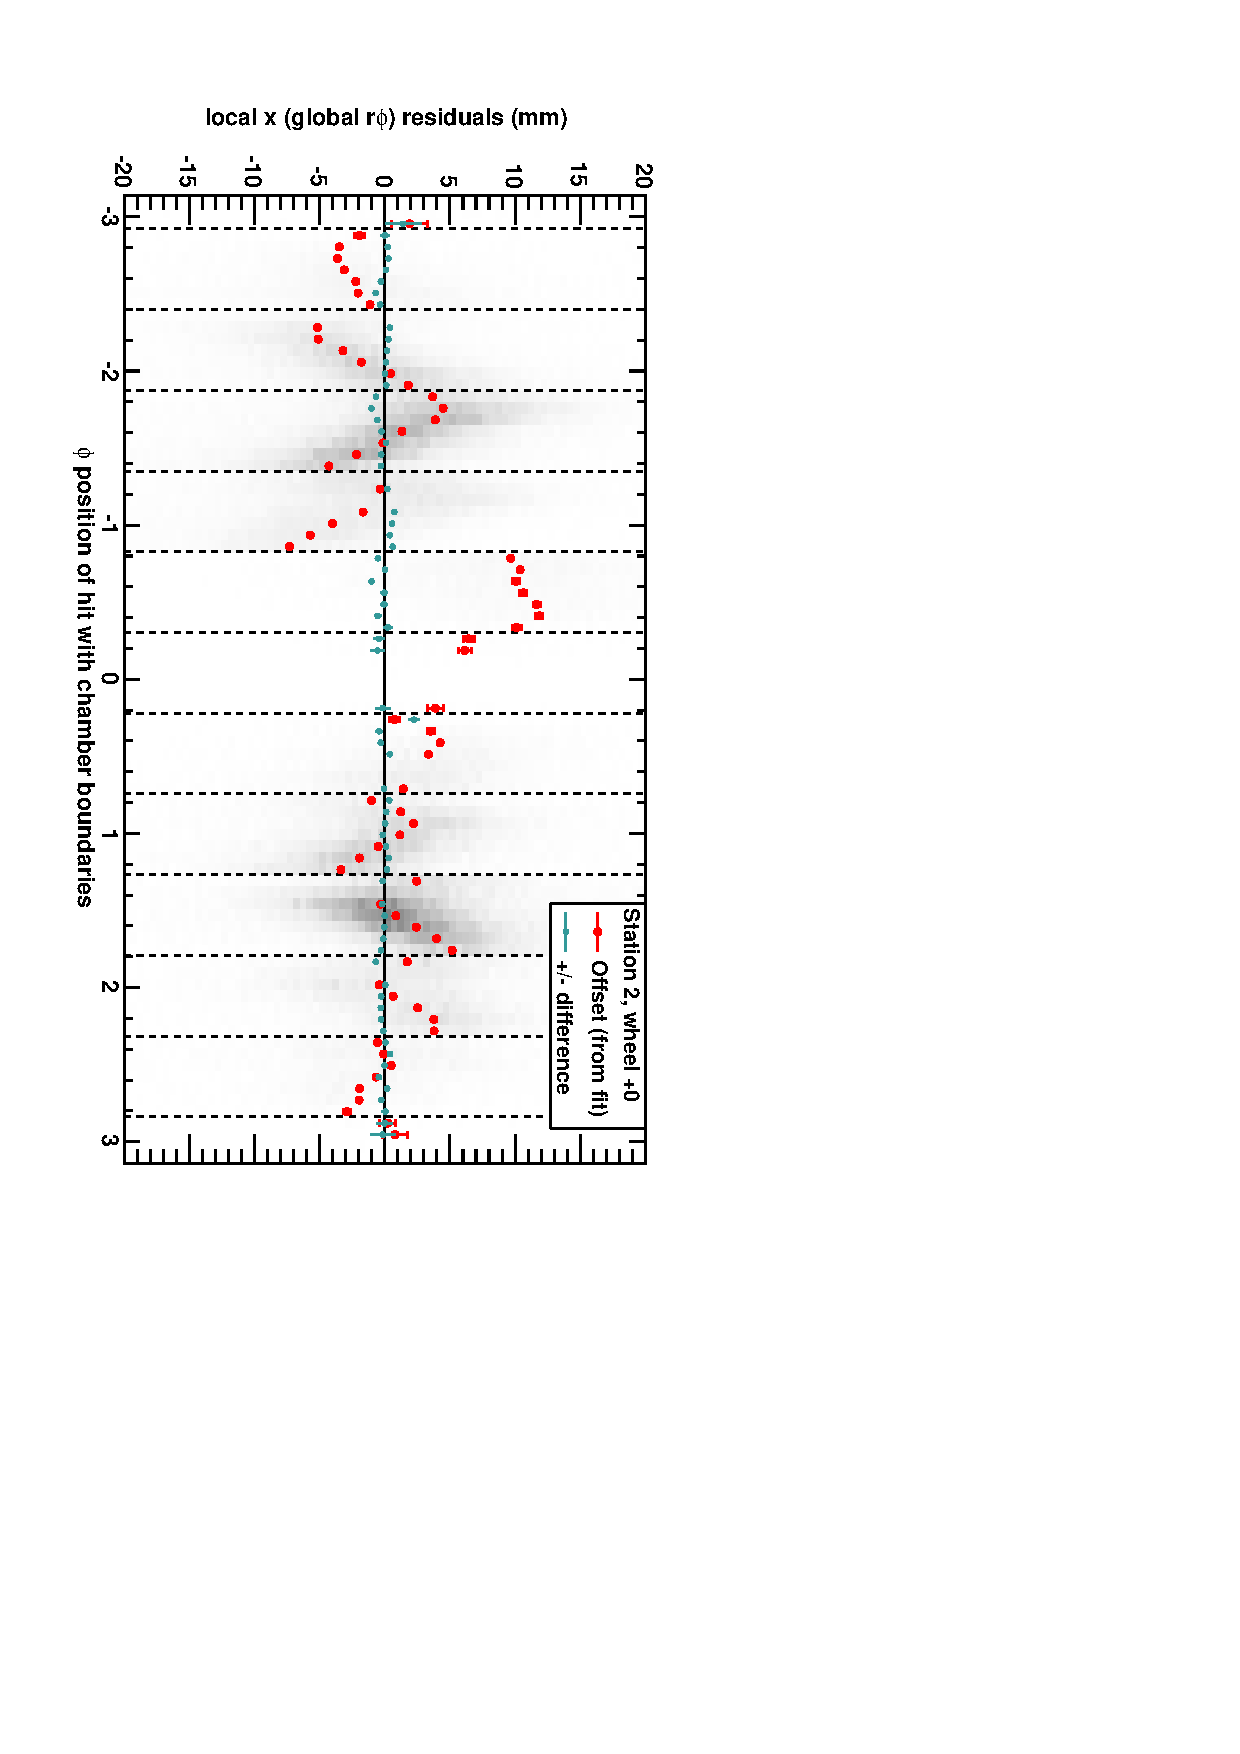
\includegraphics[height=1.2\linewidth, angle=90]{DTrphiVsPhi_st2_whC.pdf}} \end{frame}
\section*{station 2, wheel +1}
\begin{frame} \vfill \mbox{\hspace{-1 cm}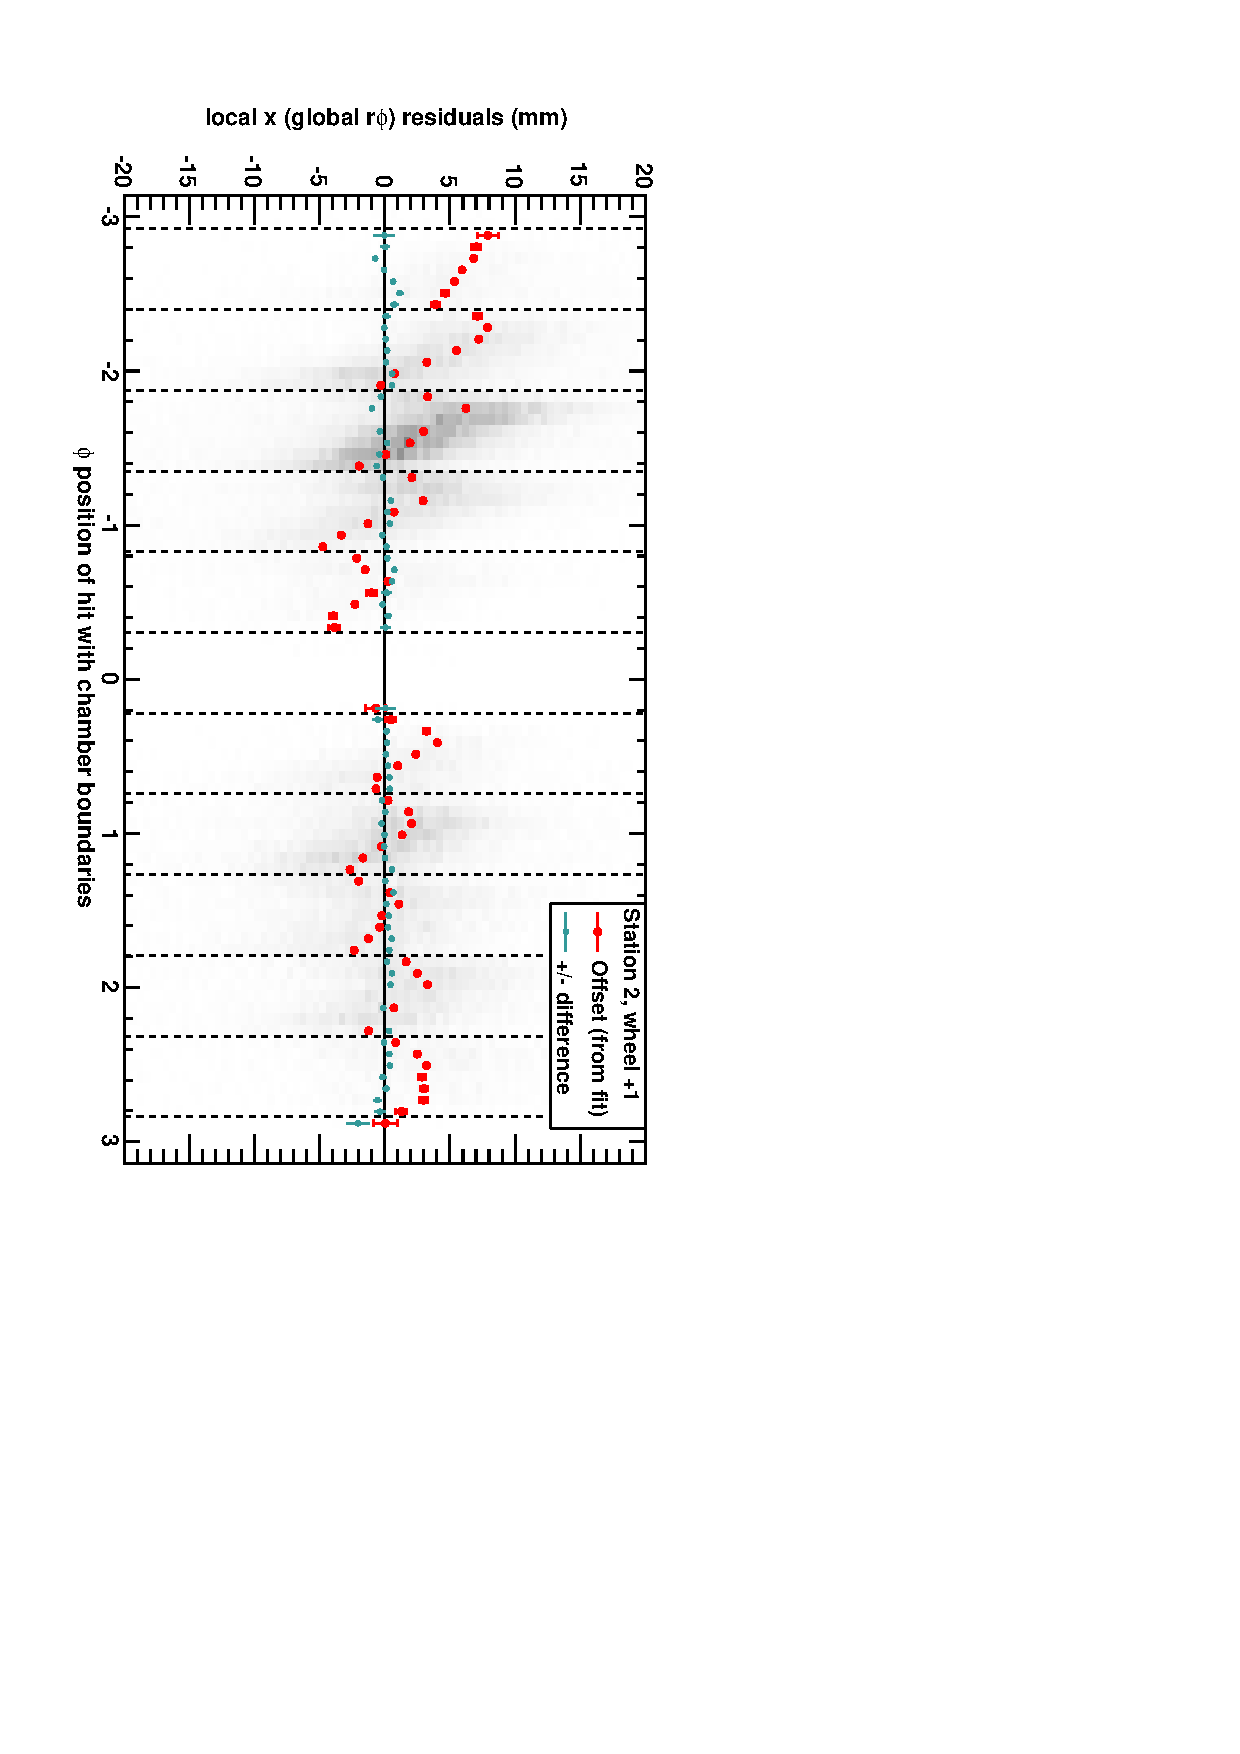
\includegraphics[height=1.2\linewidth, angle=90]{DTrphiVsPhi_st2_whD.pdf}} \end{frame}
\section*{station 2, wheel +2}
\begin{frame} \vfill \mbox{\hspace{-1 cm}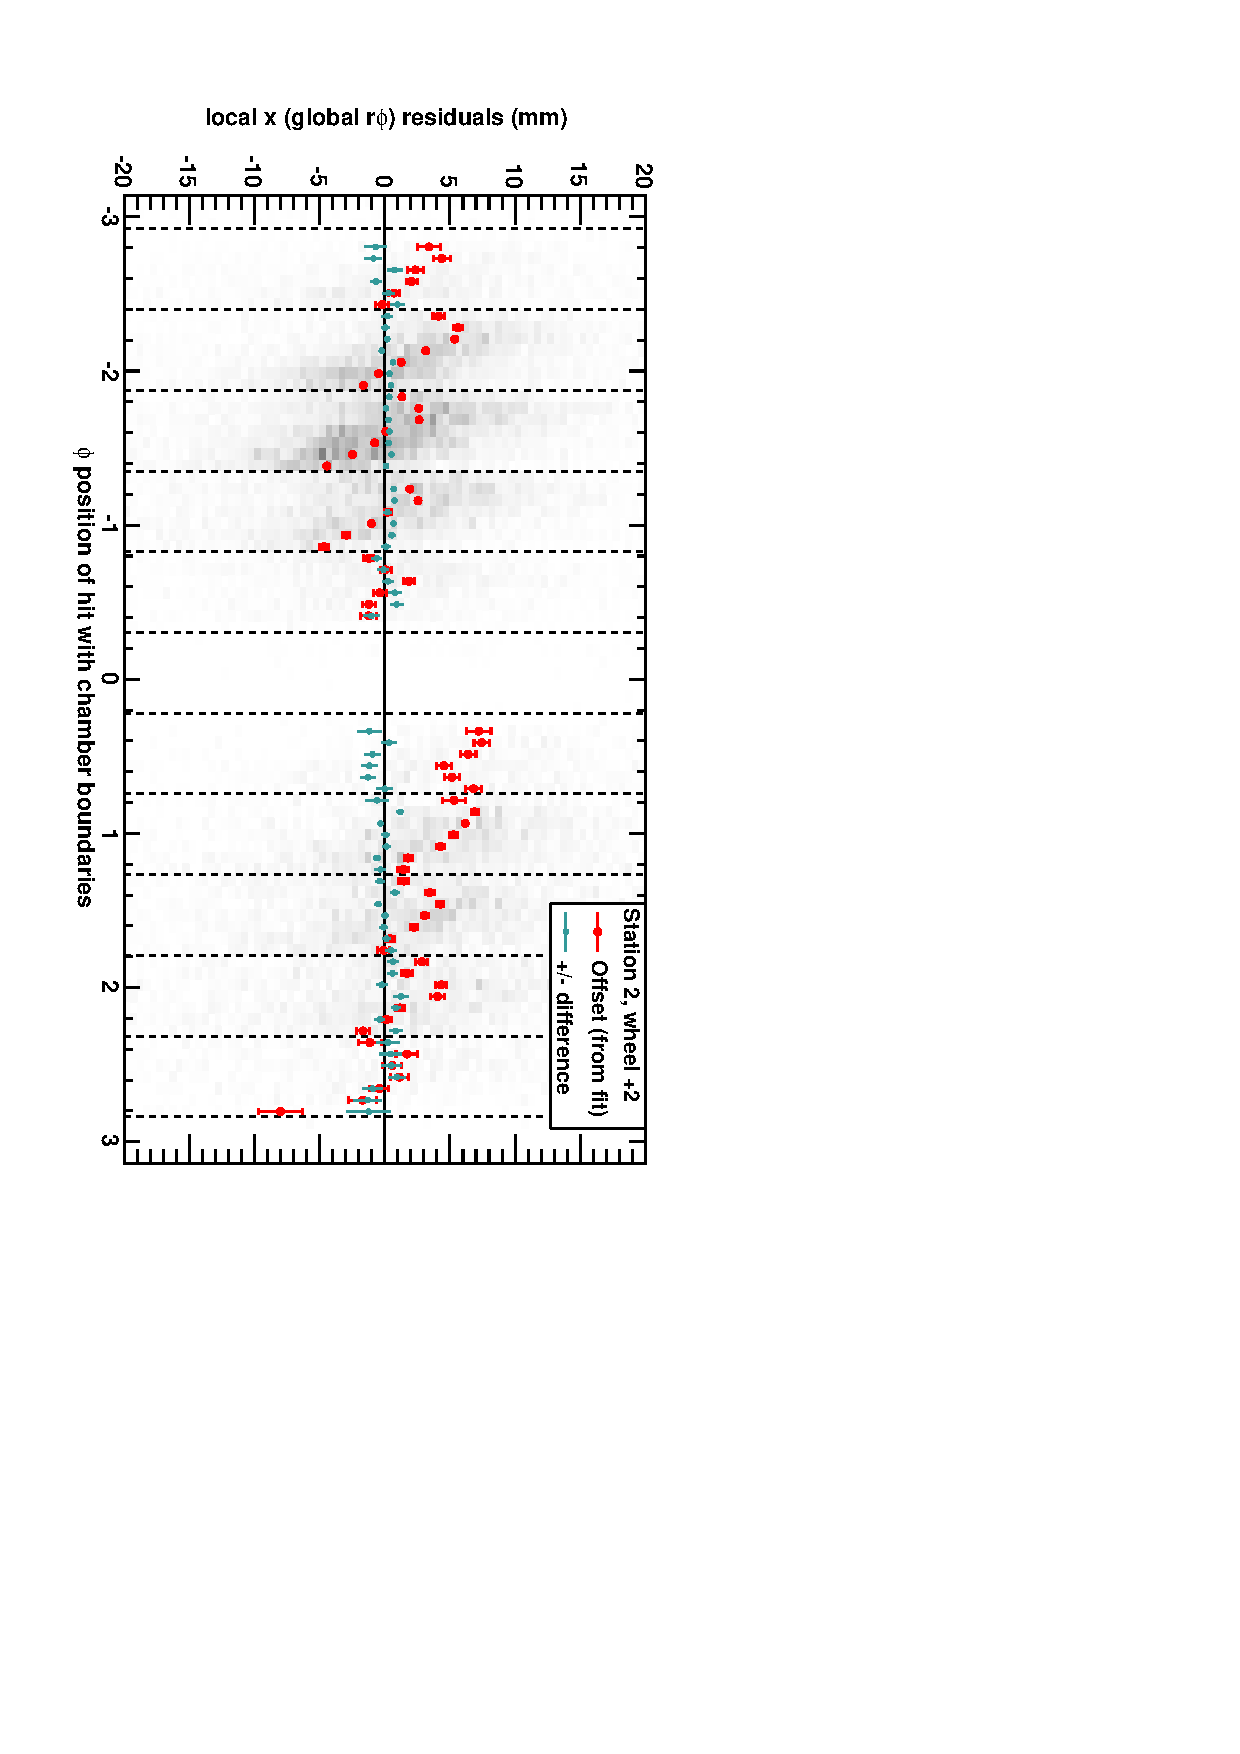
\includegraphics[height=1.2\linewidth, angle=90]{DTrphiVsPhi_st2_whE.pdf}} \end{frame}
\section*{station 3, wheel -2}
\begin{frame} \vfill \mbox{\hspace{-1 cm}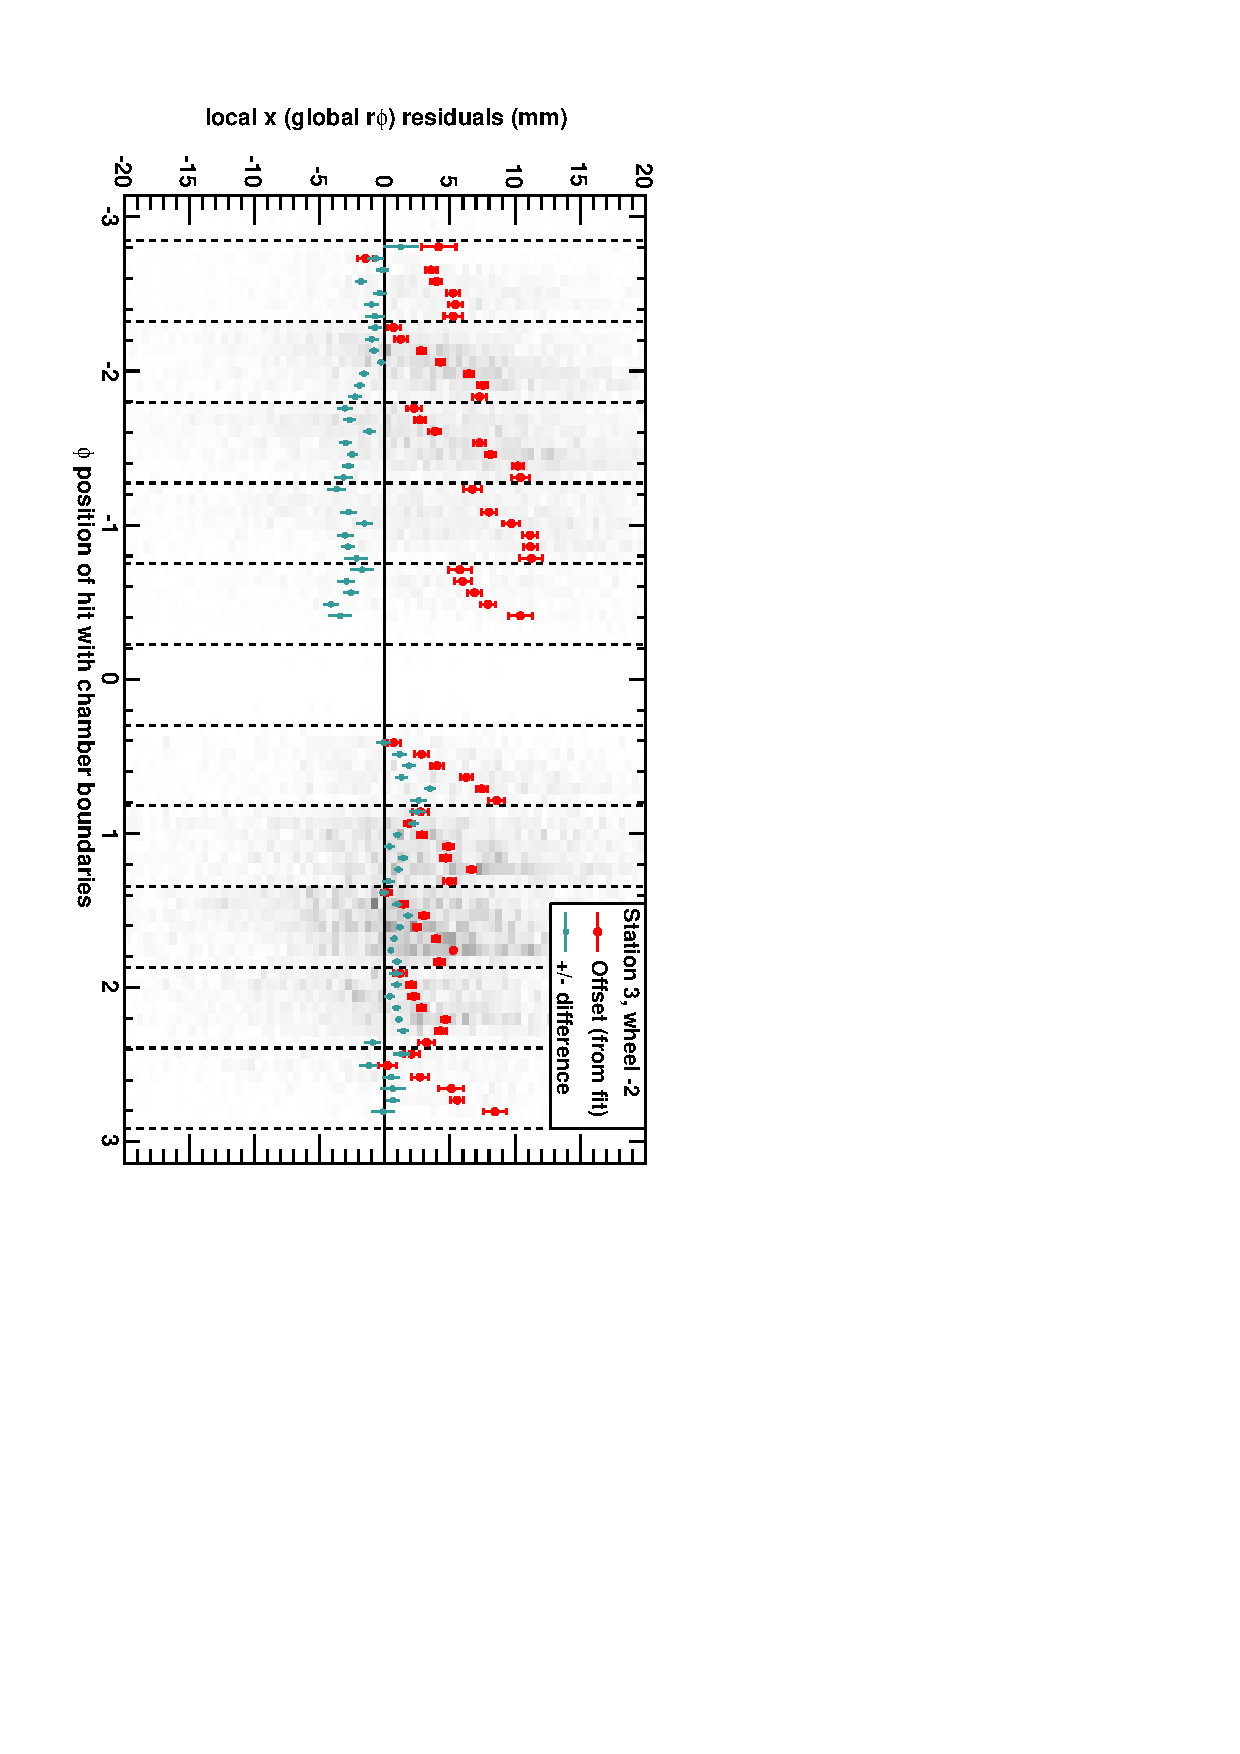
\includegraphics[height=1.2\linewidth, angle=90]{DTrphiVsPhi_st3_whA.pdf}} \end{frame}
\section*{station 3, wheel -1}
\begin{frame} \vfill \mbox{\hspace{-1 cm}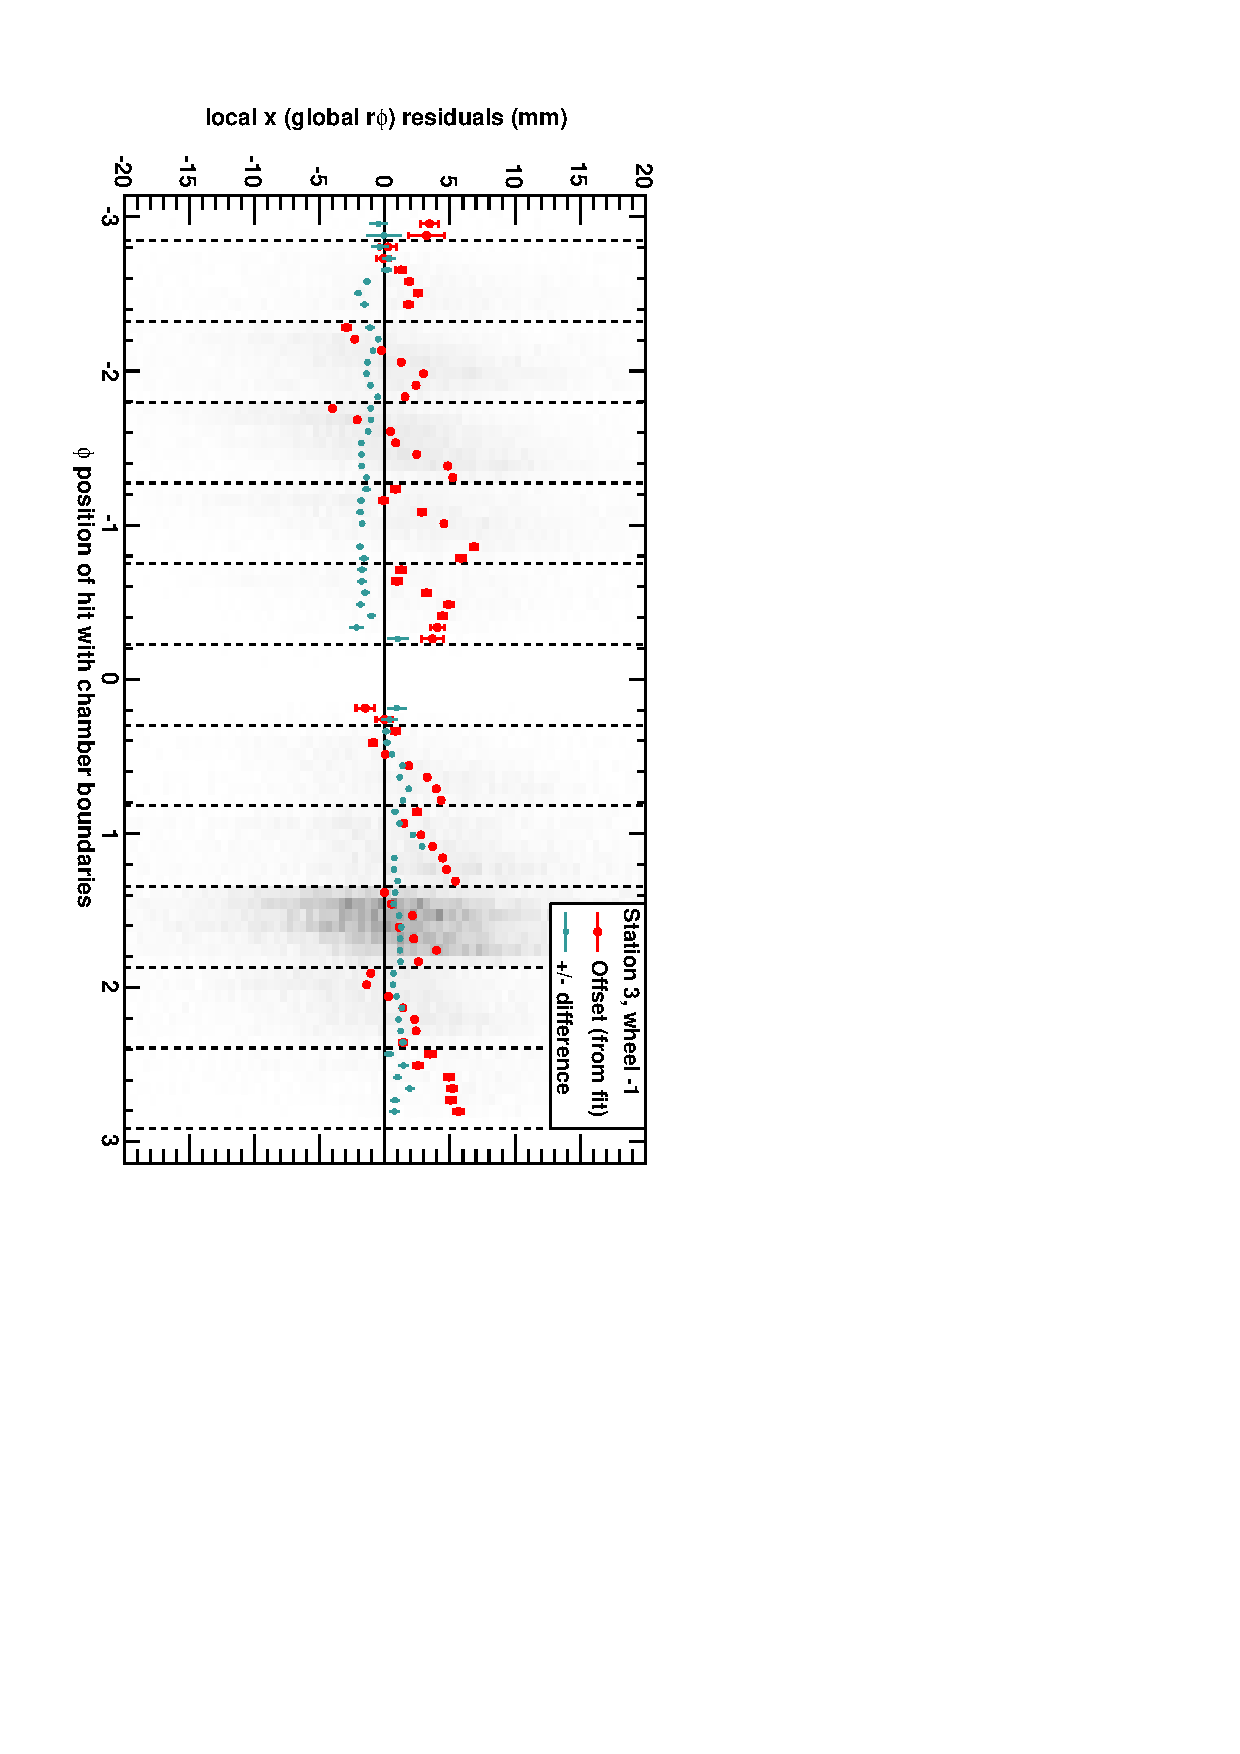
\includegraphics[height=1.2\linewidth, angle=90]{DTrphiVsPhi_st3_whB.pdf}} \end{frame}
\section*{station 3, wheel 0}
\begin{frame} \vfill \mbox{\hspace{-1 cm}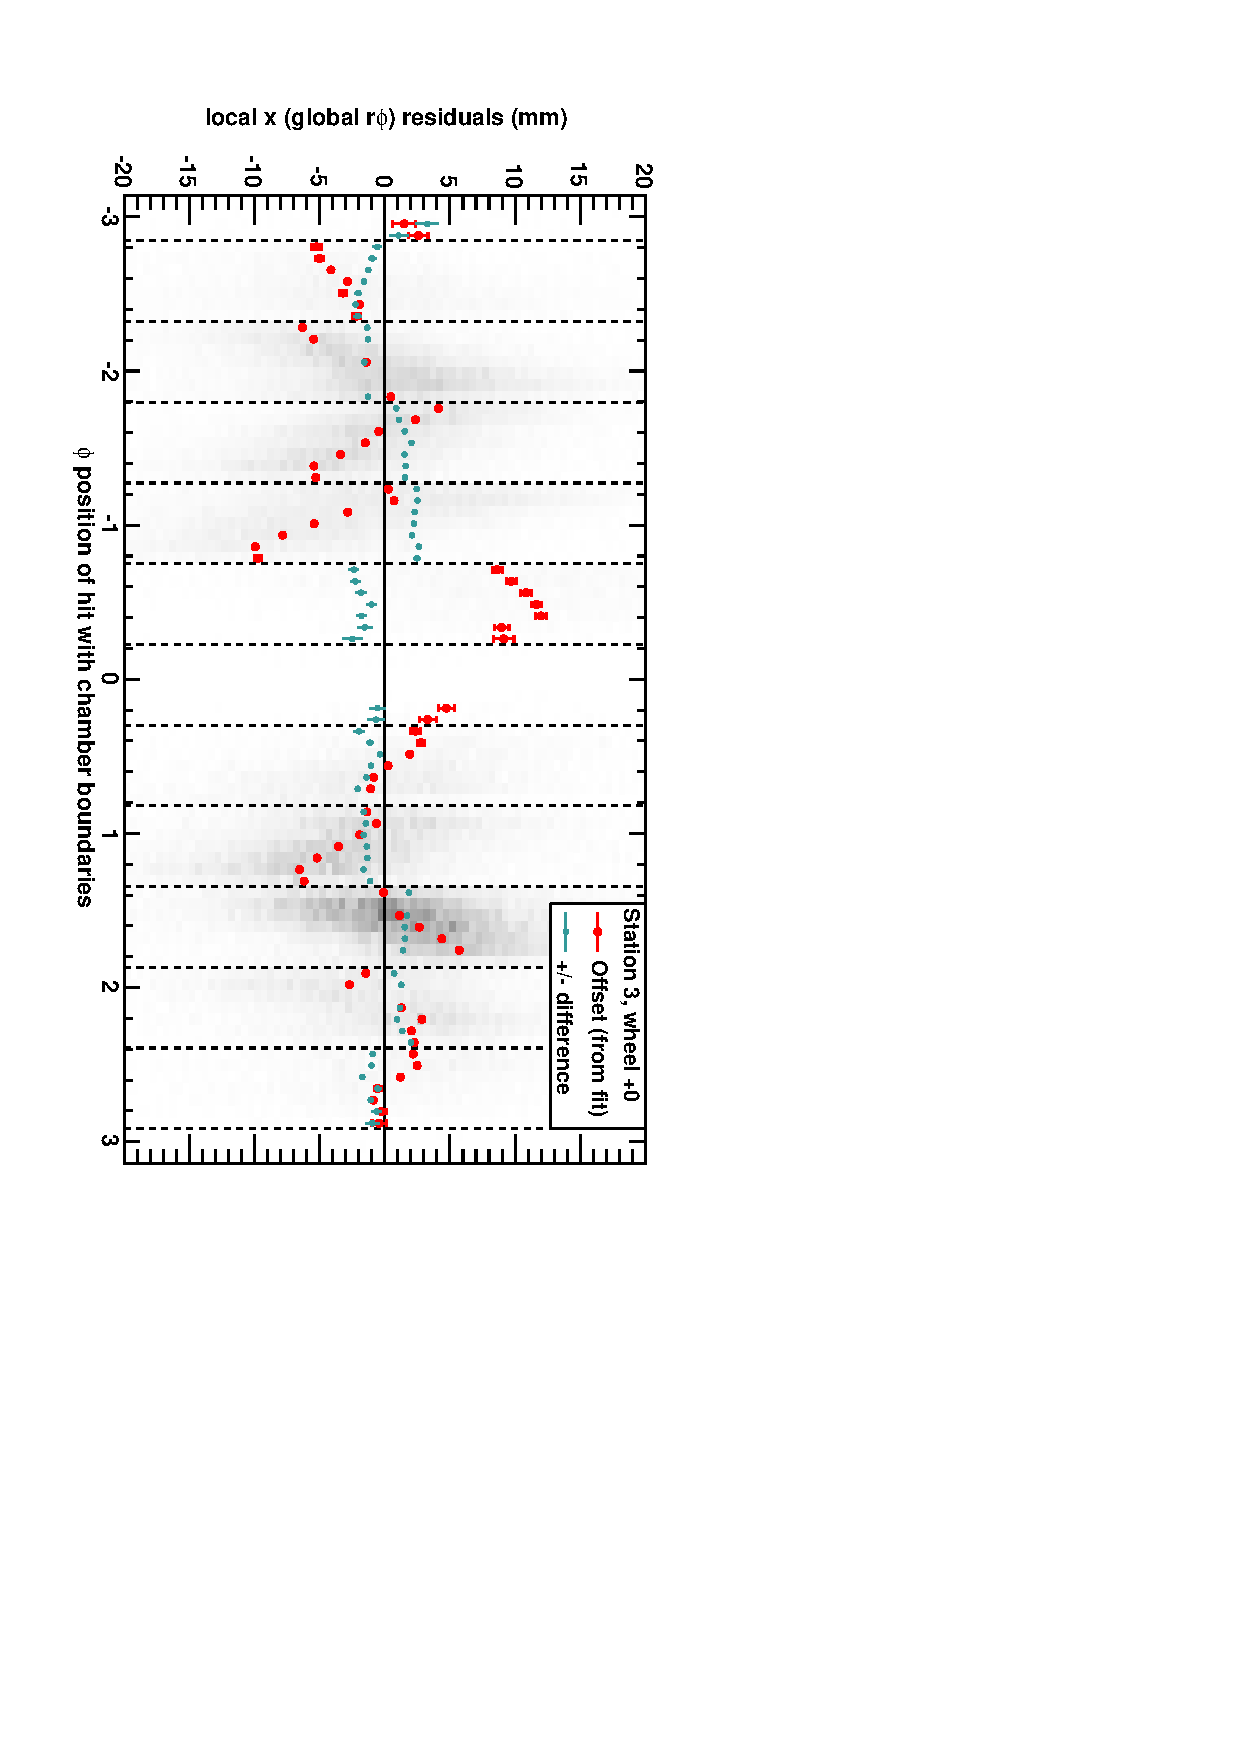
\includegraphics[height=1.2\linewidth, angle=90]{DTrphiVsPhi_st3_whC.pdf}} \end{frame}
\section*{station 3, wheel +1}
\begin{frame} \vfill \mbox{\hspace{-1 cm}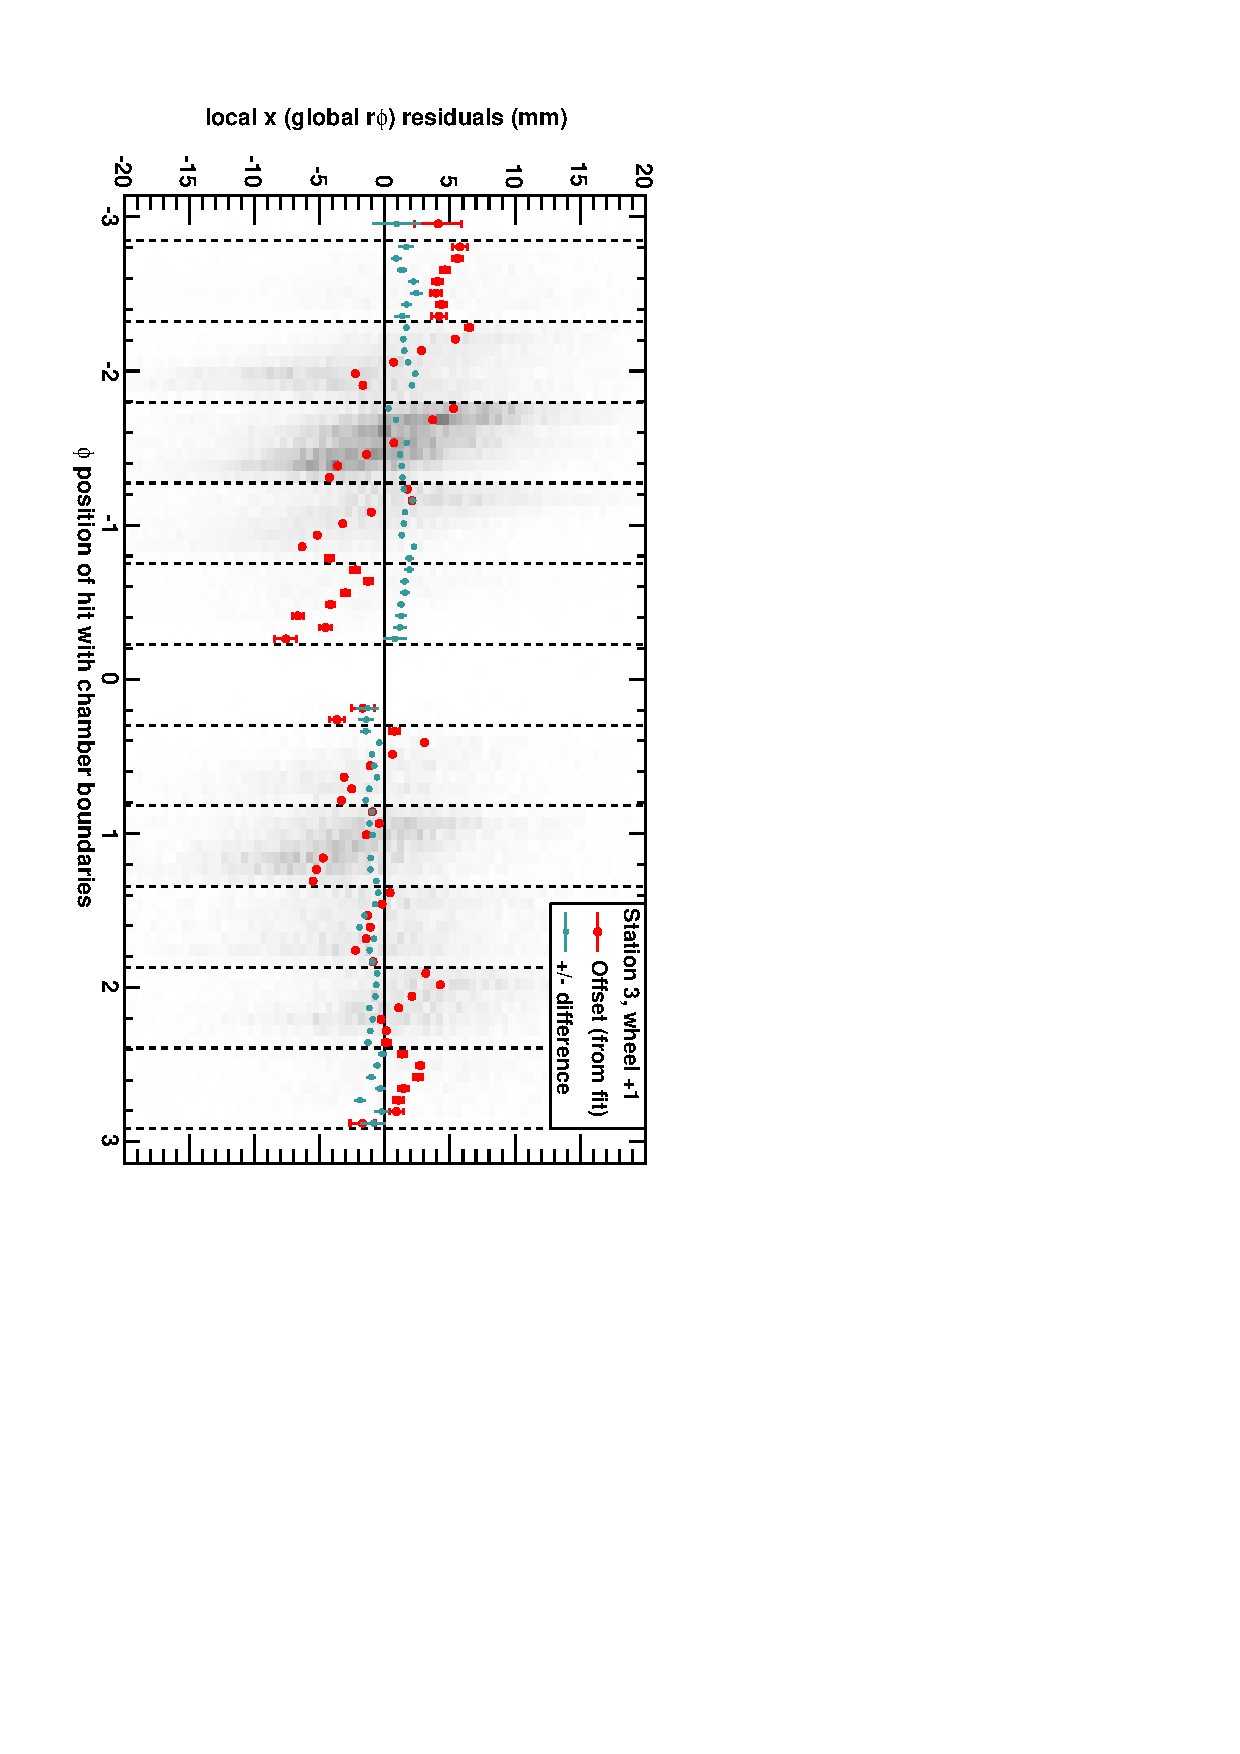
\includegraphics[height=1.2\linewidth, angle=90]{DTrphiVsPhi_st3_whD.pdf}} \end{frame}
\section*{station 3, wheel +2}
\begin{frame} \vfill \mbox{\hspace{-1 cm}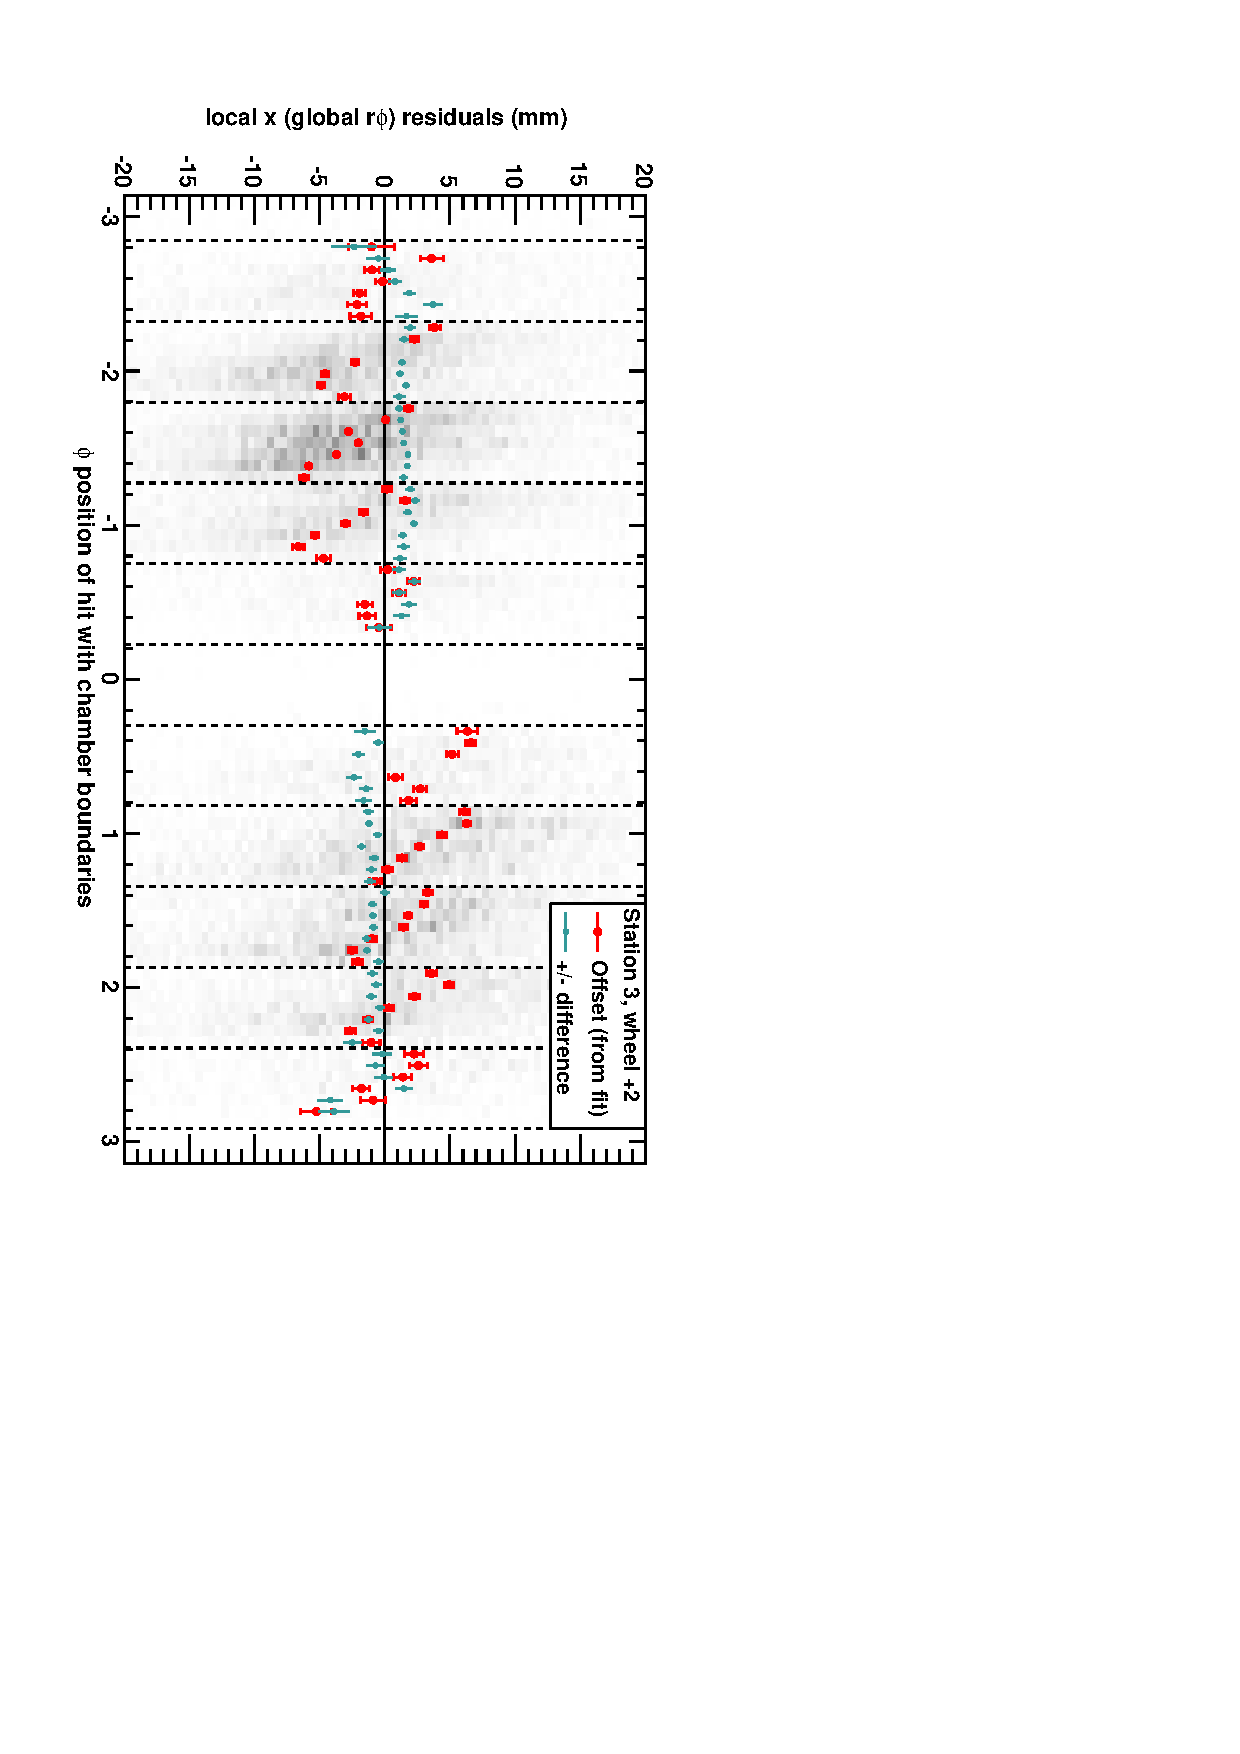
\includegraphics[height=1.2\linewidth, angle=90]{DTrphiVsPhi_st3_whE.pdf}} \end{frame}
\section*{station 4, wheel -2}
\begin{frame} \vfill \mbox{\hspace{-1 cm}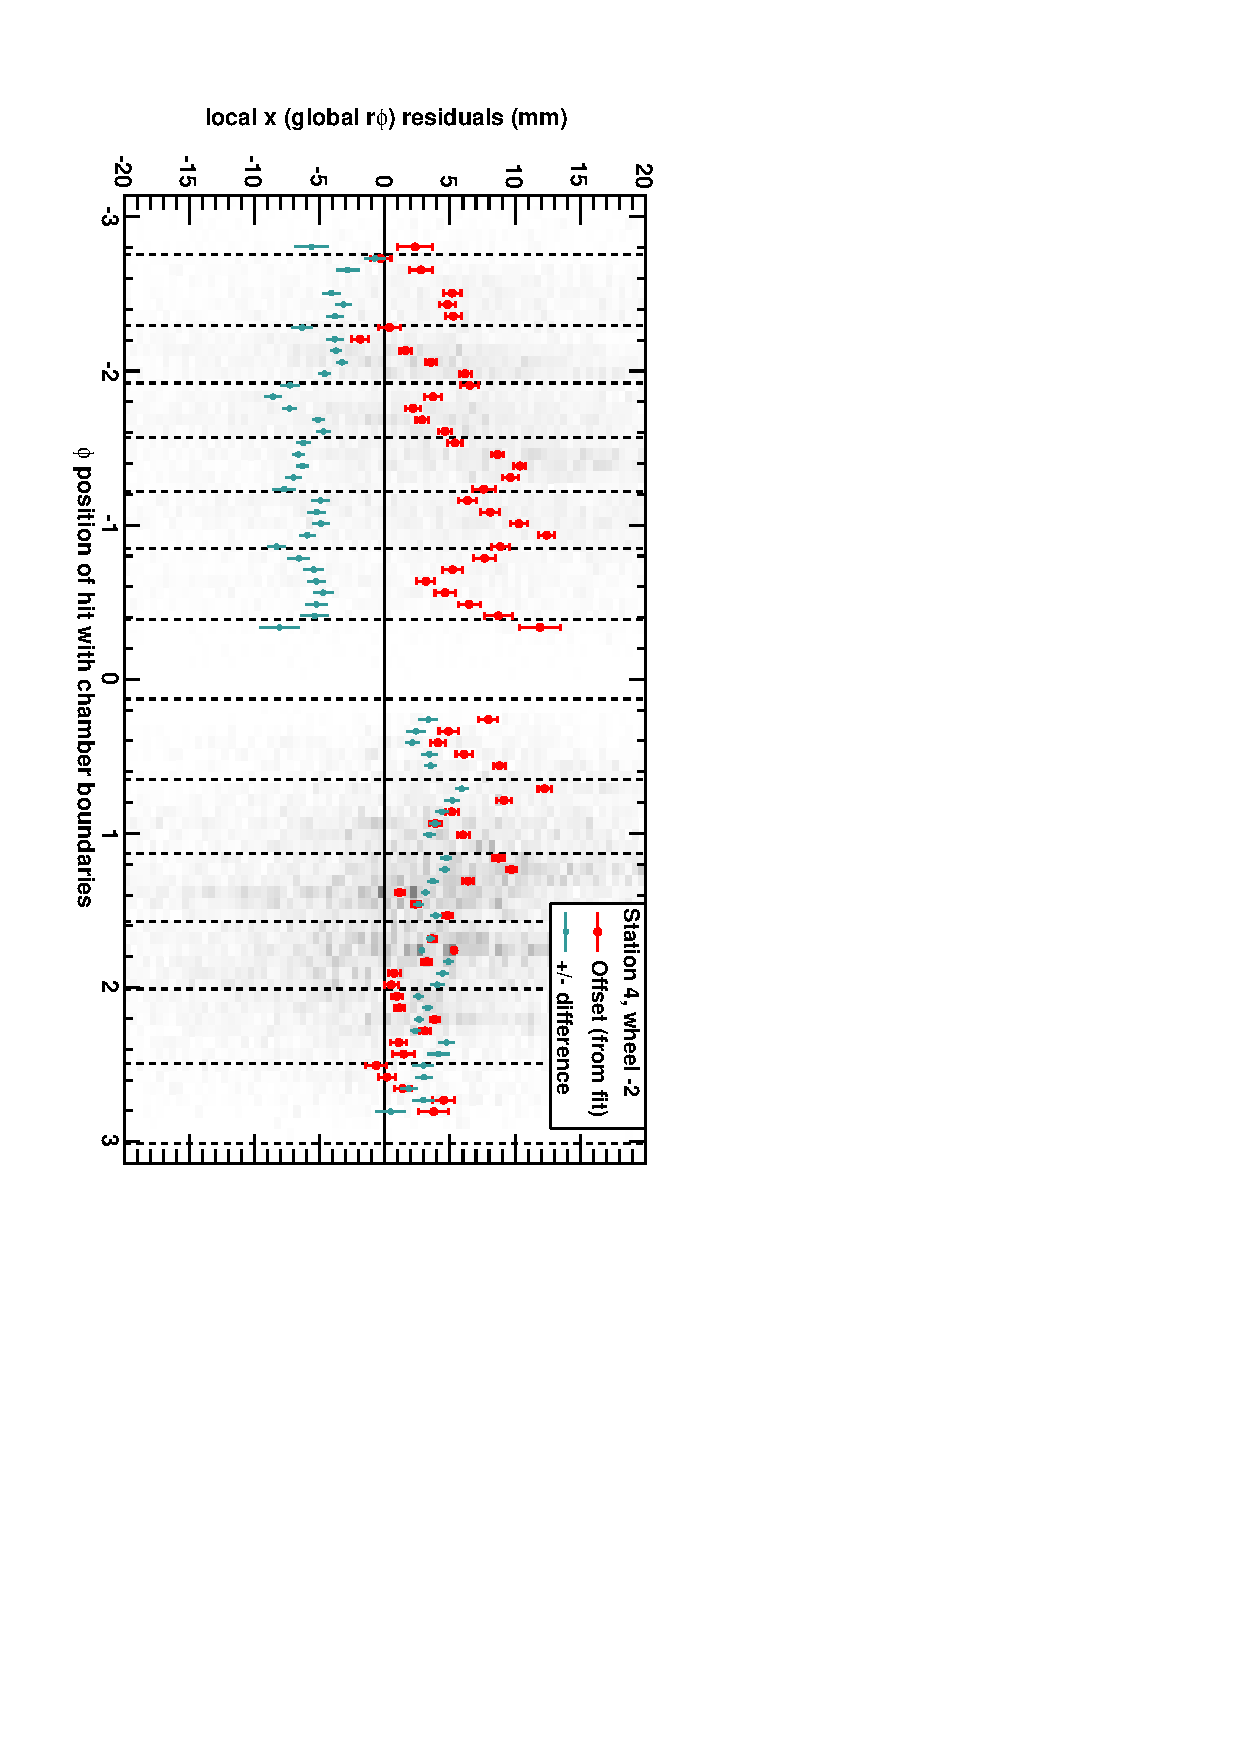
\includegraphics[height=1.2\linewidth, angle=90]{DTrphiVsPhi_st4_whA.pdf}} \end{frame}
\section*{station 4, wheel -1}
\begin{frame} \vfill \mbox{\hspace{-1 cm}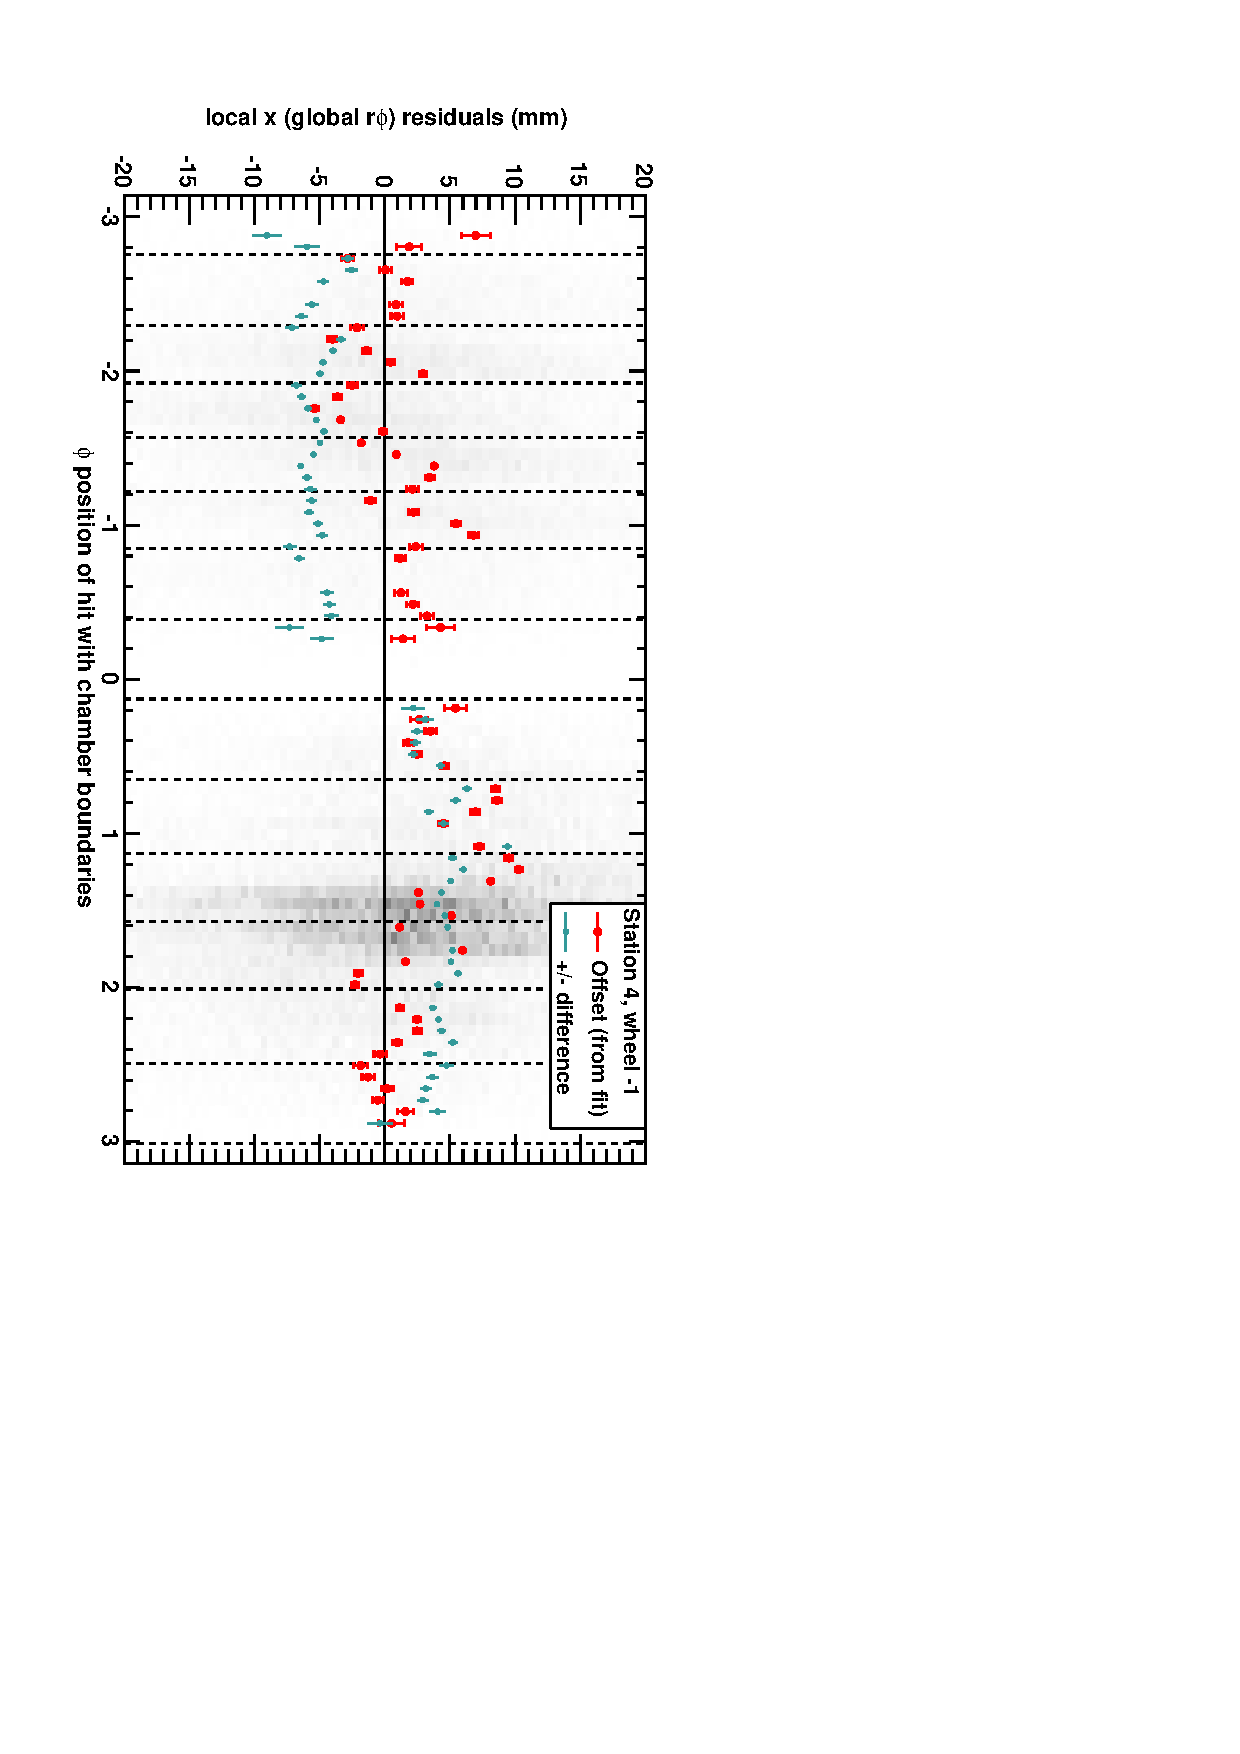
\includegraphics[height=1.2\linewidth, angle=90]{DTrphiVsPhi_st4_whB.pdf}} \end{frame}
\section*{station 4, wheel 0}
\begin{frame} \vfill \mbox{\hspace{-1 cm}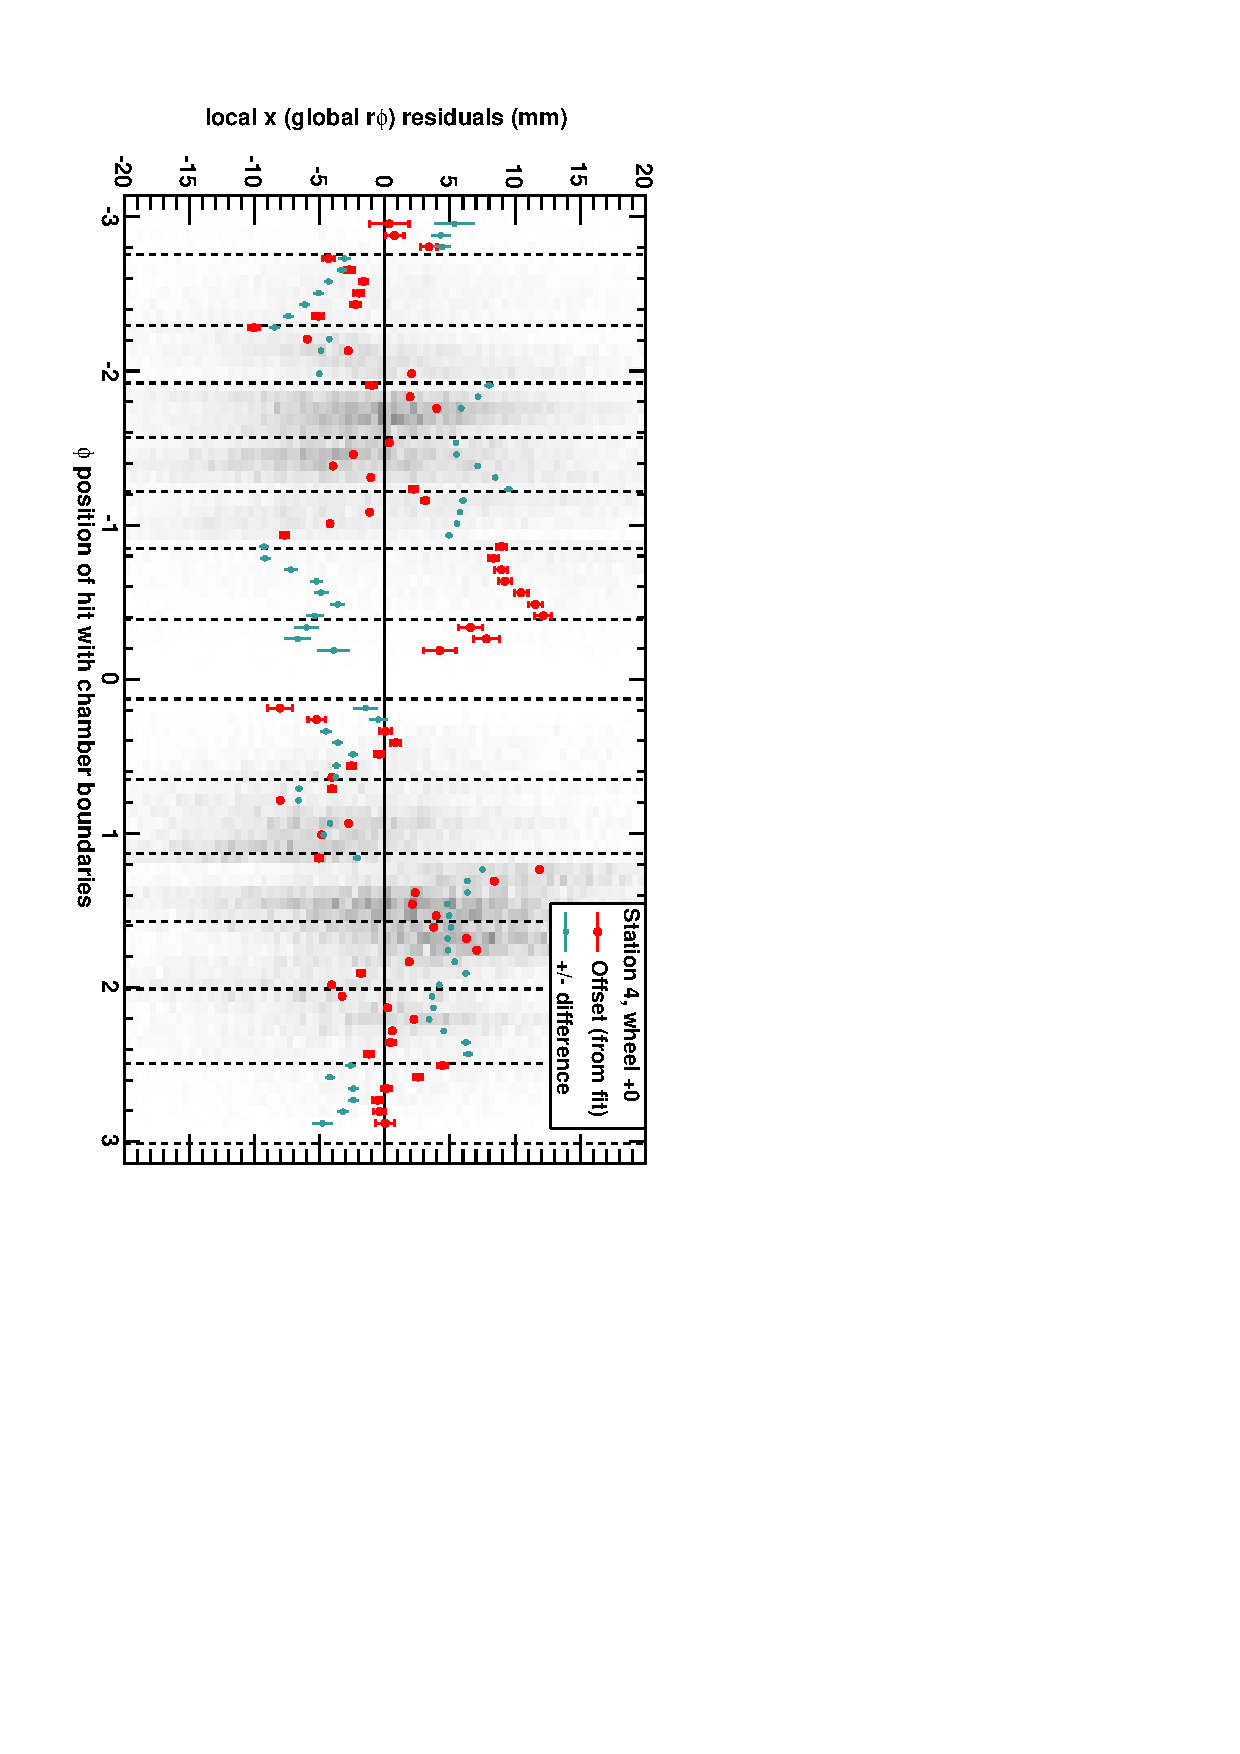
\includegraphics[height=1.2\linewidth, angle=90]{DTrphiVsPhi_st4_whC.pdf}} \end{frame}
\section*{station 4, wheel +1}
\begin{frame} \vfill \mbox{\hspace{-1 cm}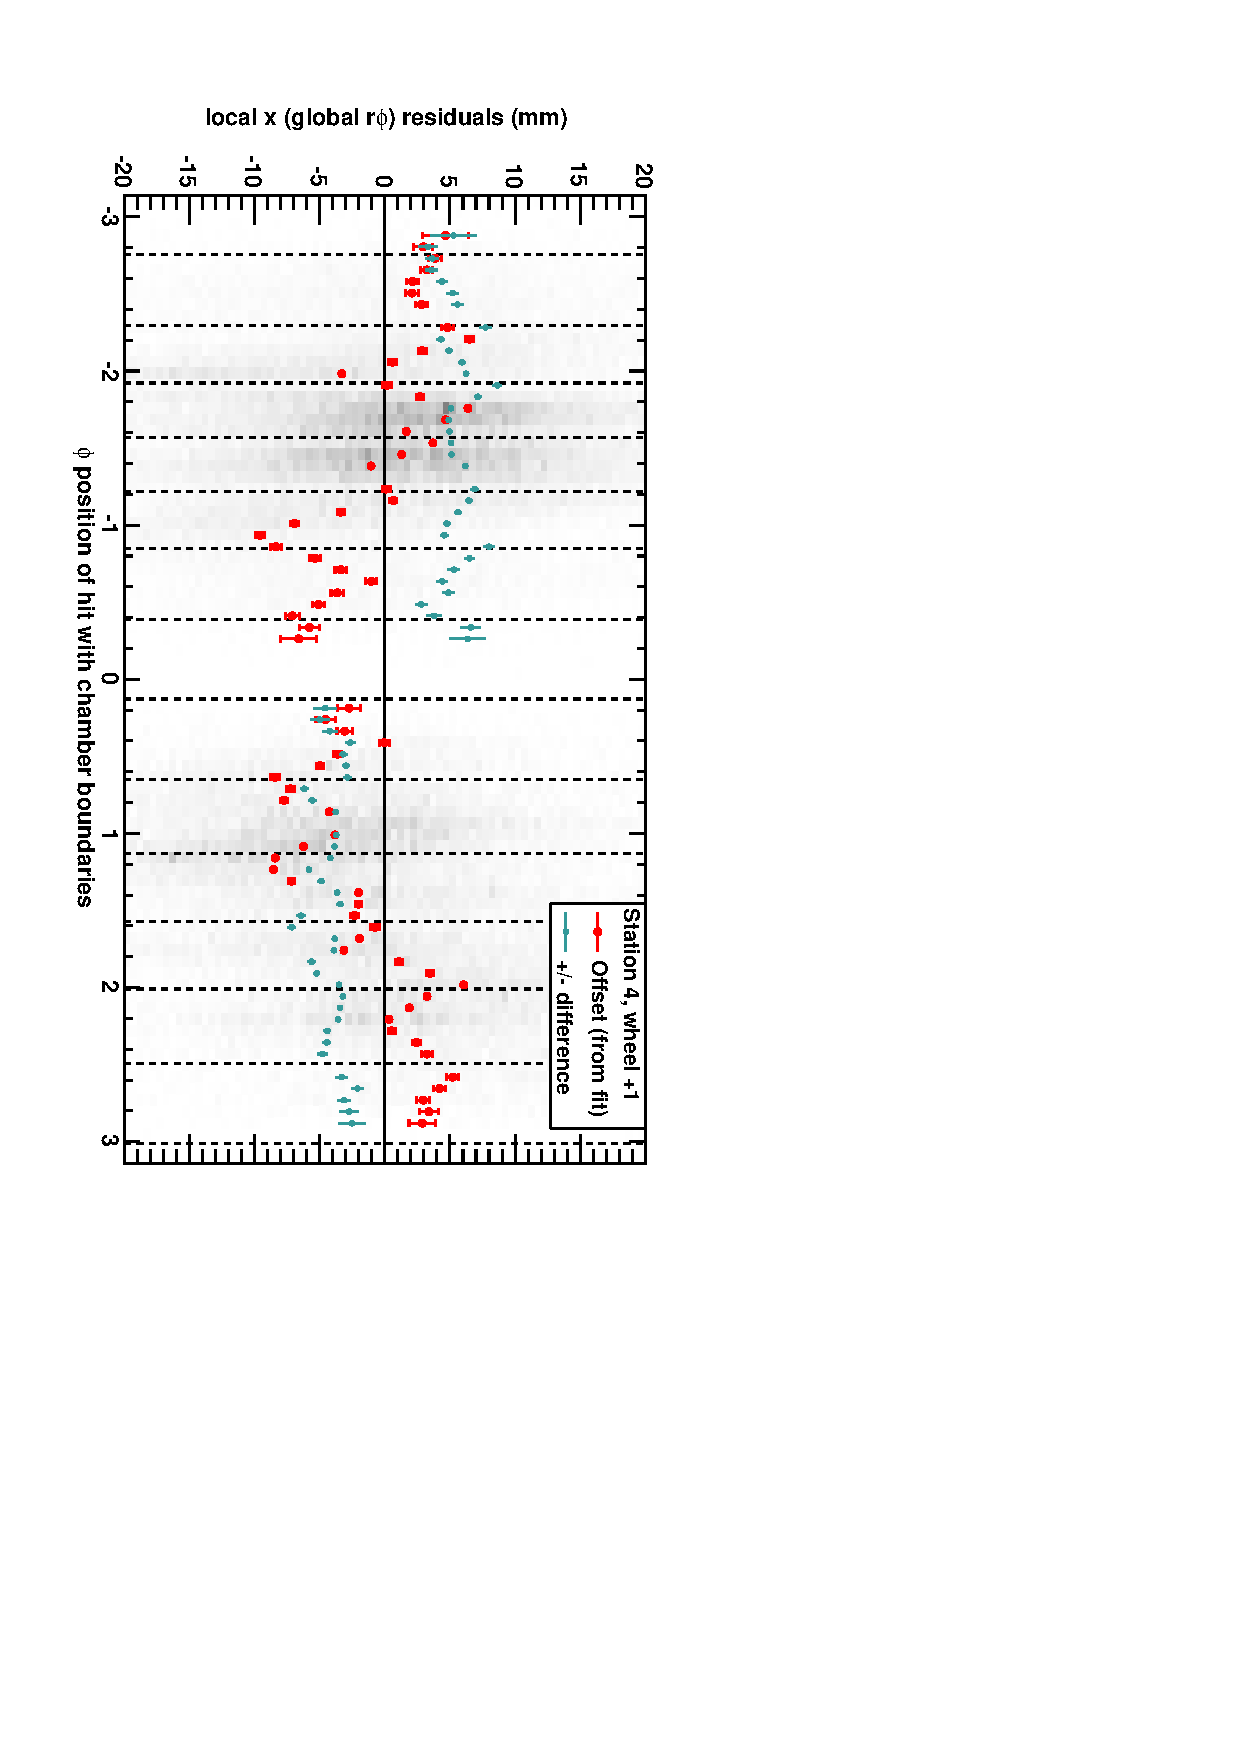
\includegraphics[height=1.2\linewidth, angle=90]{DTrphiVsPhi_st4_whD.pdf}} \end{frame}
\section*{station 4, wheel +2}
\begin{frame} \vfill \mbox{\hspace{-1 cm}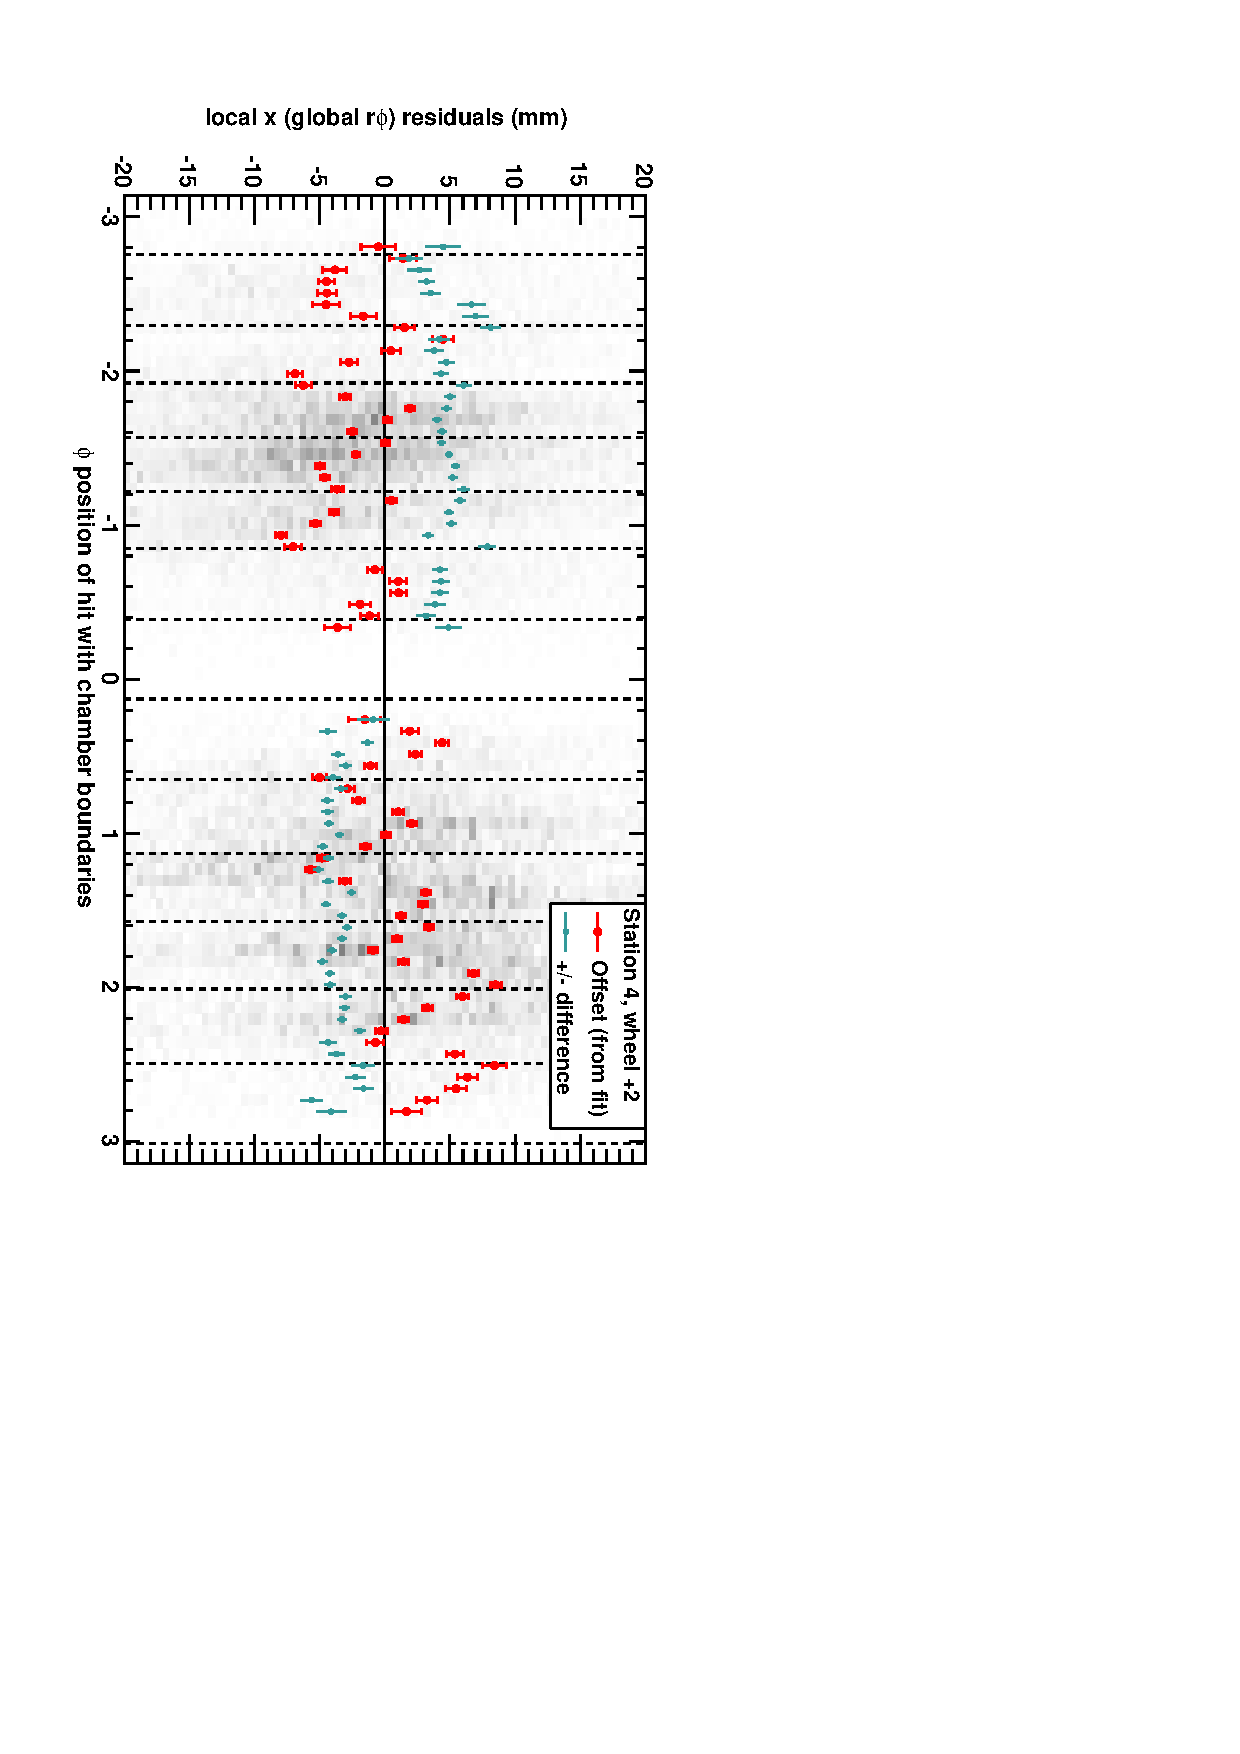
\includegraphics[height=1.2\linewidth, angle=90]{DTrphiVsPhi_st4_whE.pdf}} \end{frame}

\section*{Rphi residuals versus z}
\begin{frame}
\begin{center}
\Huge \textcolor{blue}{$r\phi$ residuals versus $z$}
\end{center}
\end{frame}

\section*{station 1, sector 1}
\begin{frame} \vfill \mbox{\hspace{-1 cm}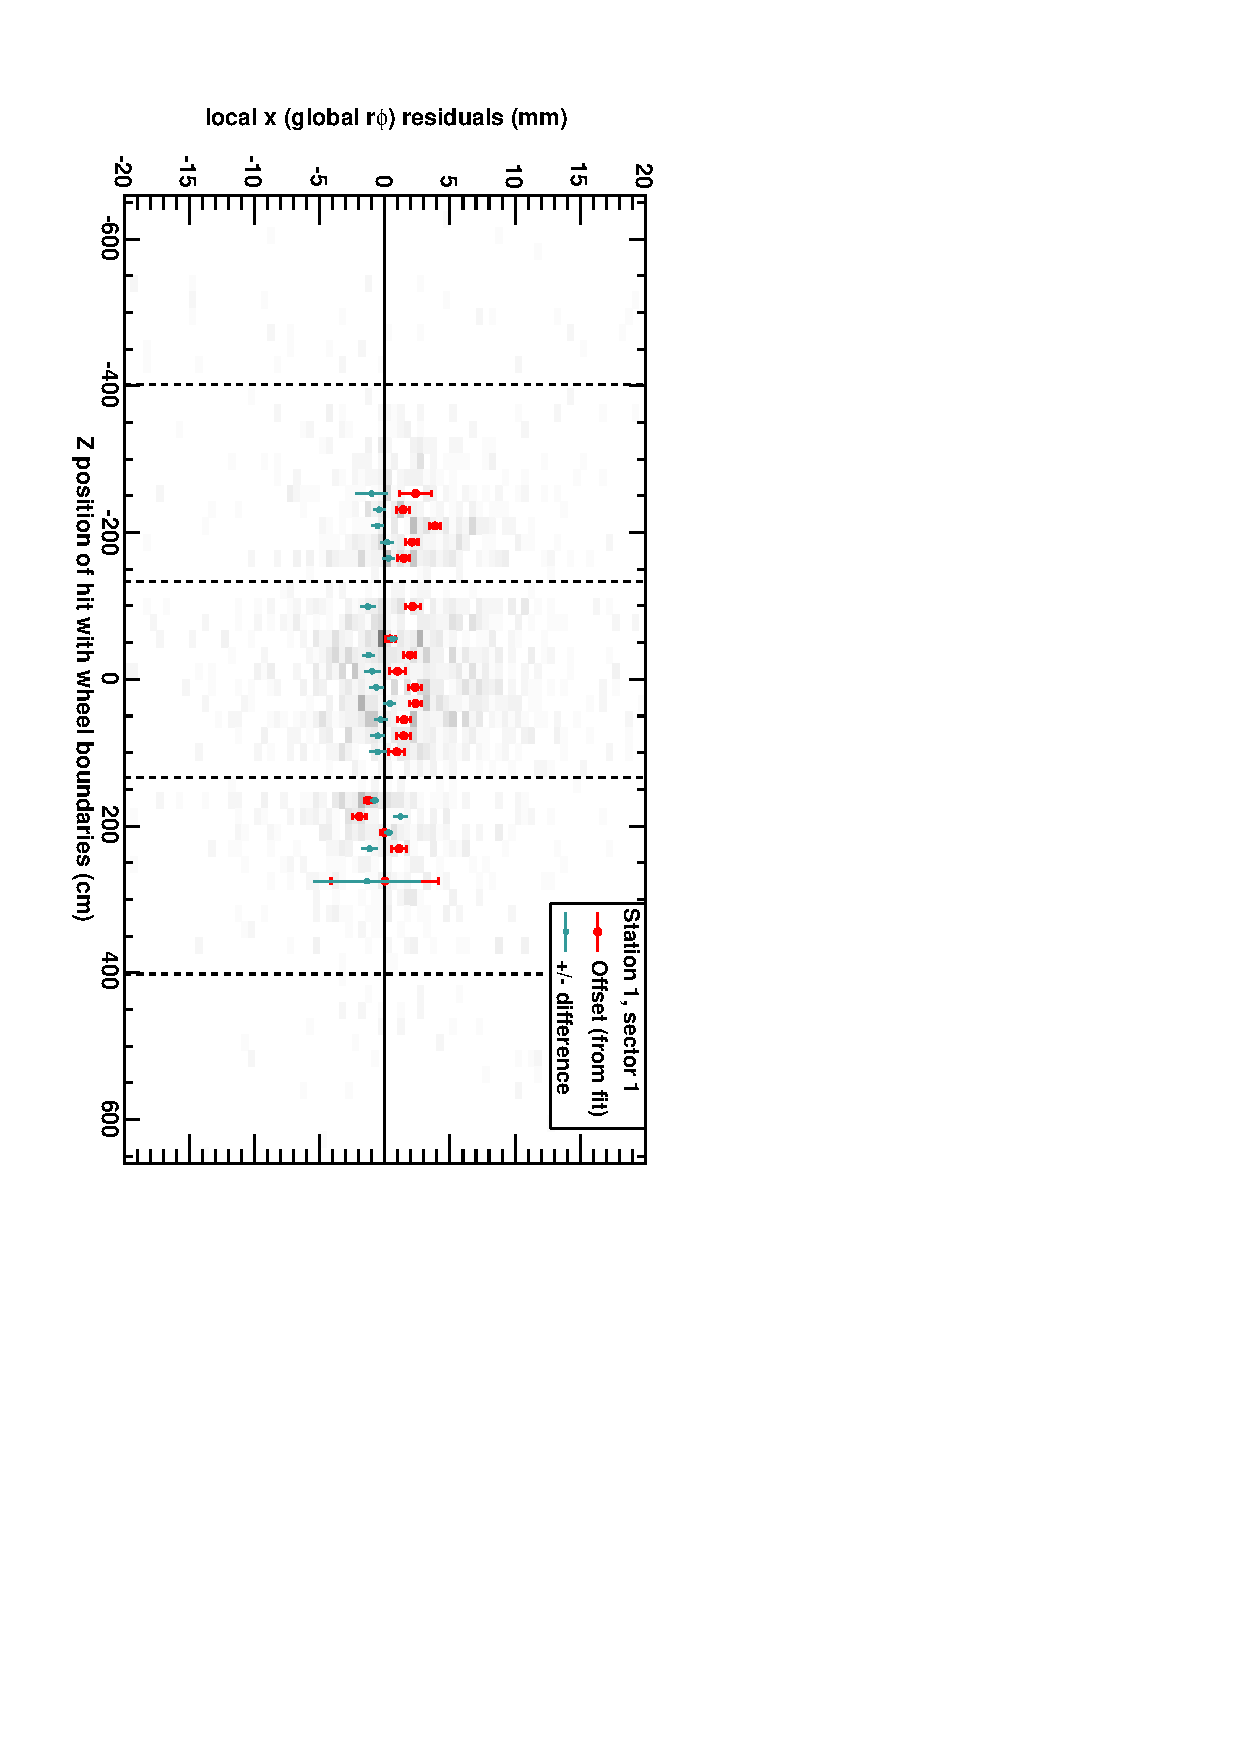
\includegraphics[height=1.2\linewidth, angle=90]{DTrphiVsZ_st1_sr01.pdf}} \end{frame}
\section*{station 1, sector 2}
\begin{frame} \vfill \mbox{\hspace{-1 cm}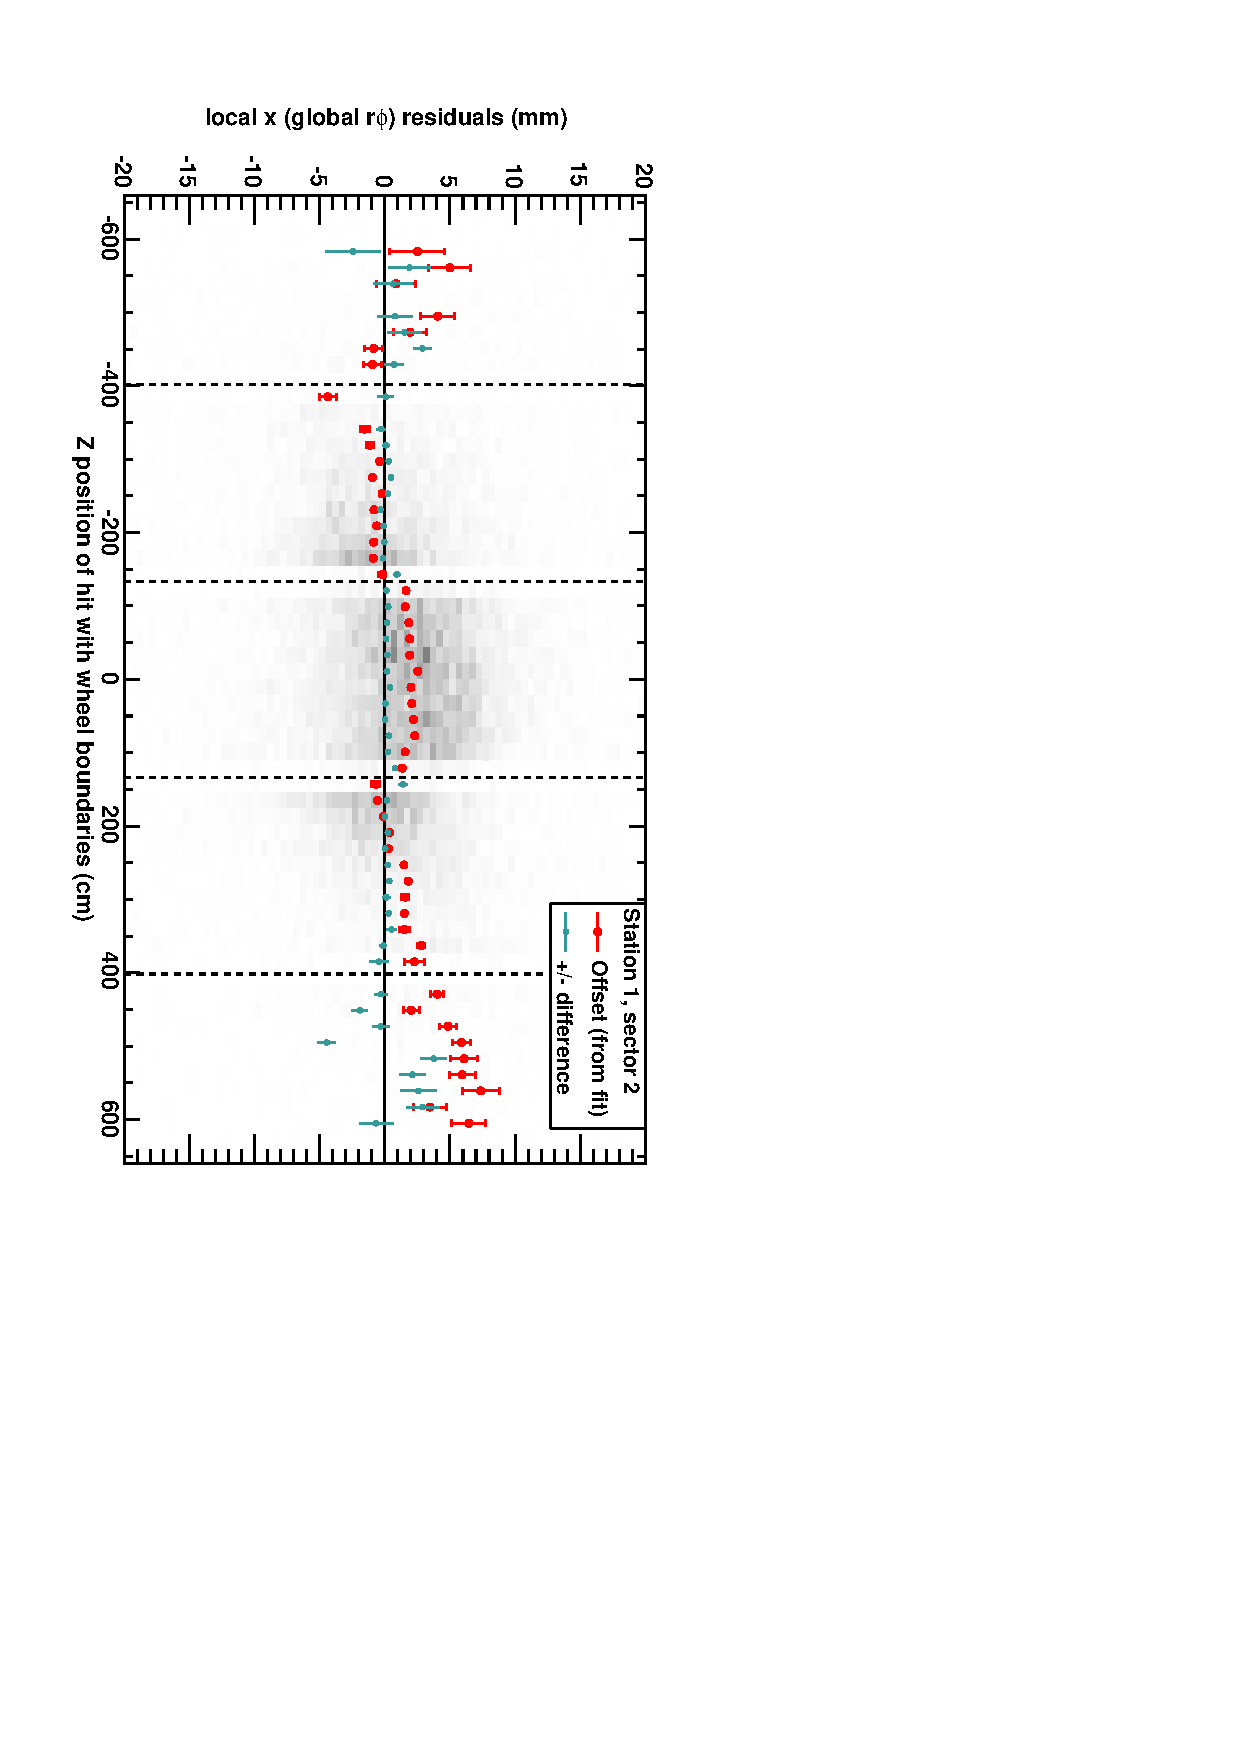
\includegraphics[height=1.2\linewidth, angle=90]{DTrphiVsZ_st1_sr02.pdf}} \end{frame}
\section*{station 1, sector 3}
\begin{frame} \vfill \mbox{\hspace{-1 cm}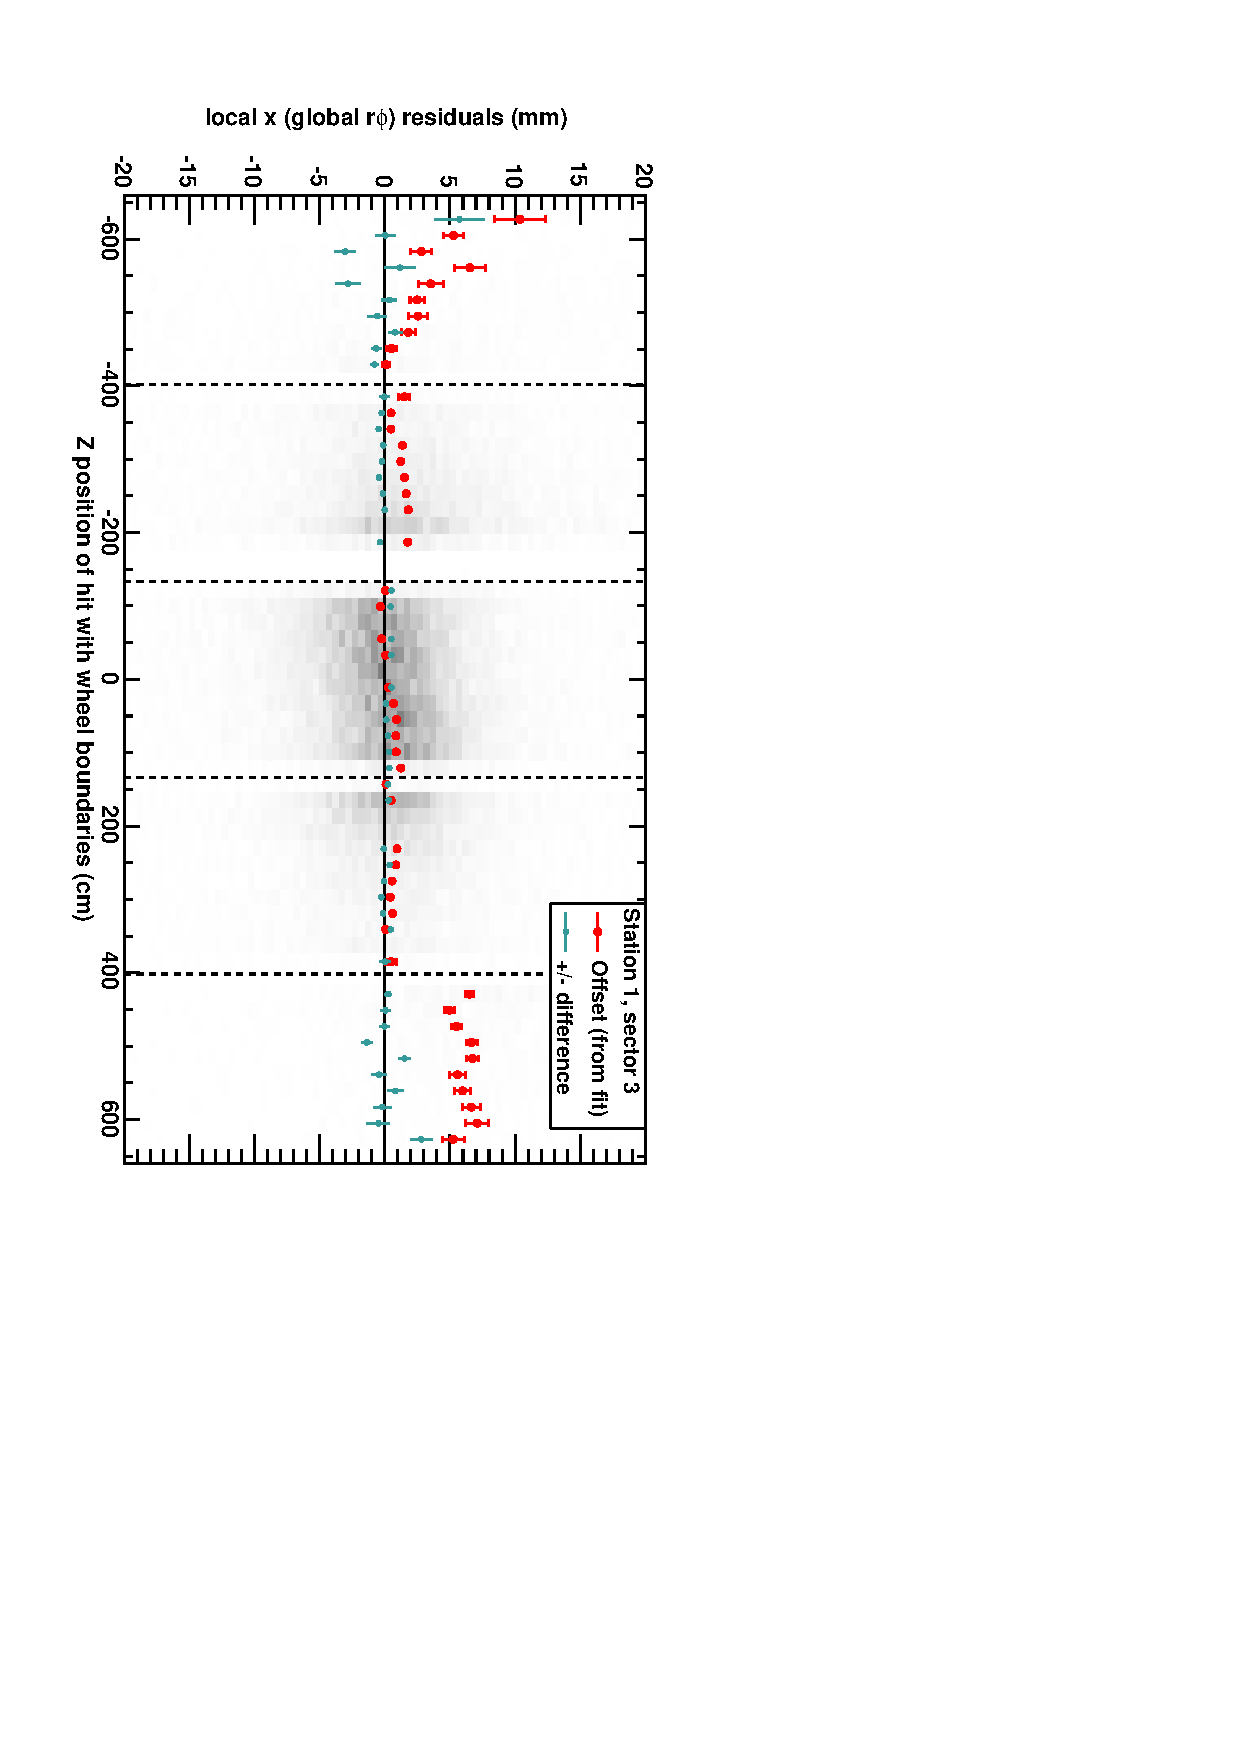
\includegraphics[height=1.2\linewidth, angle=90]{DTrphiVsZ_st1_sr03.pdf}} \end{frame}
\section*{station 1, sector 4}
\begin{frame} \vfill \mbox{\hspace{-1 cm}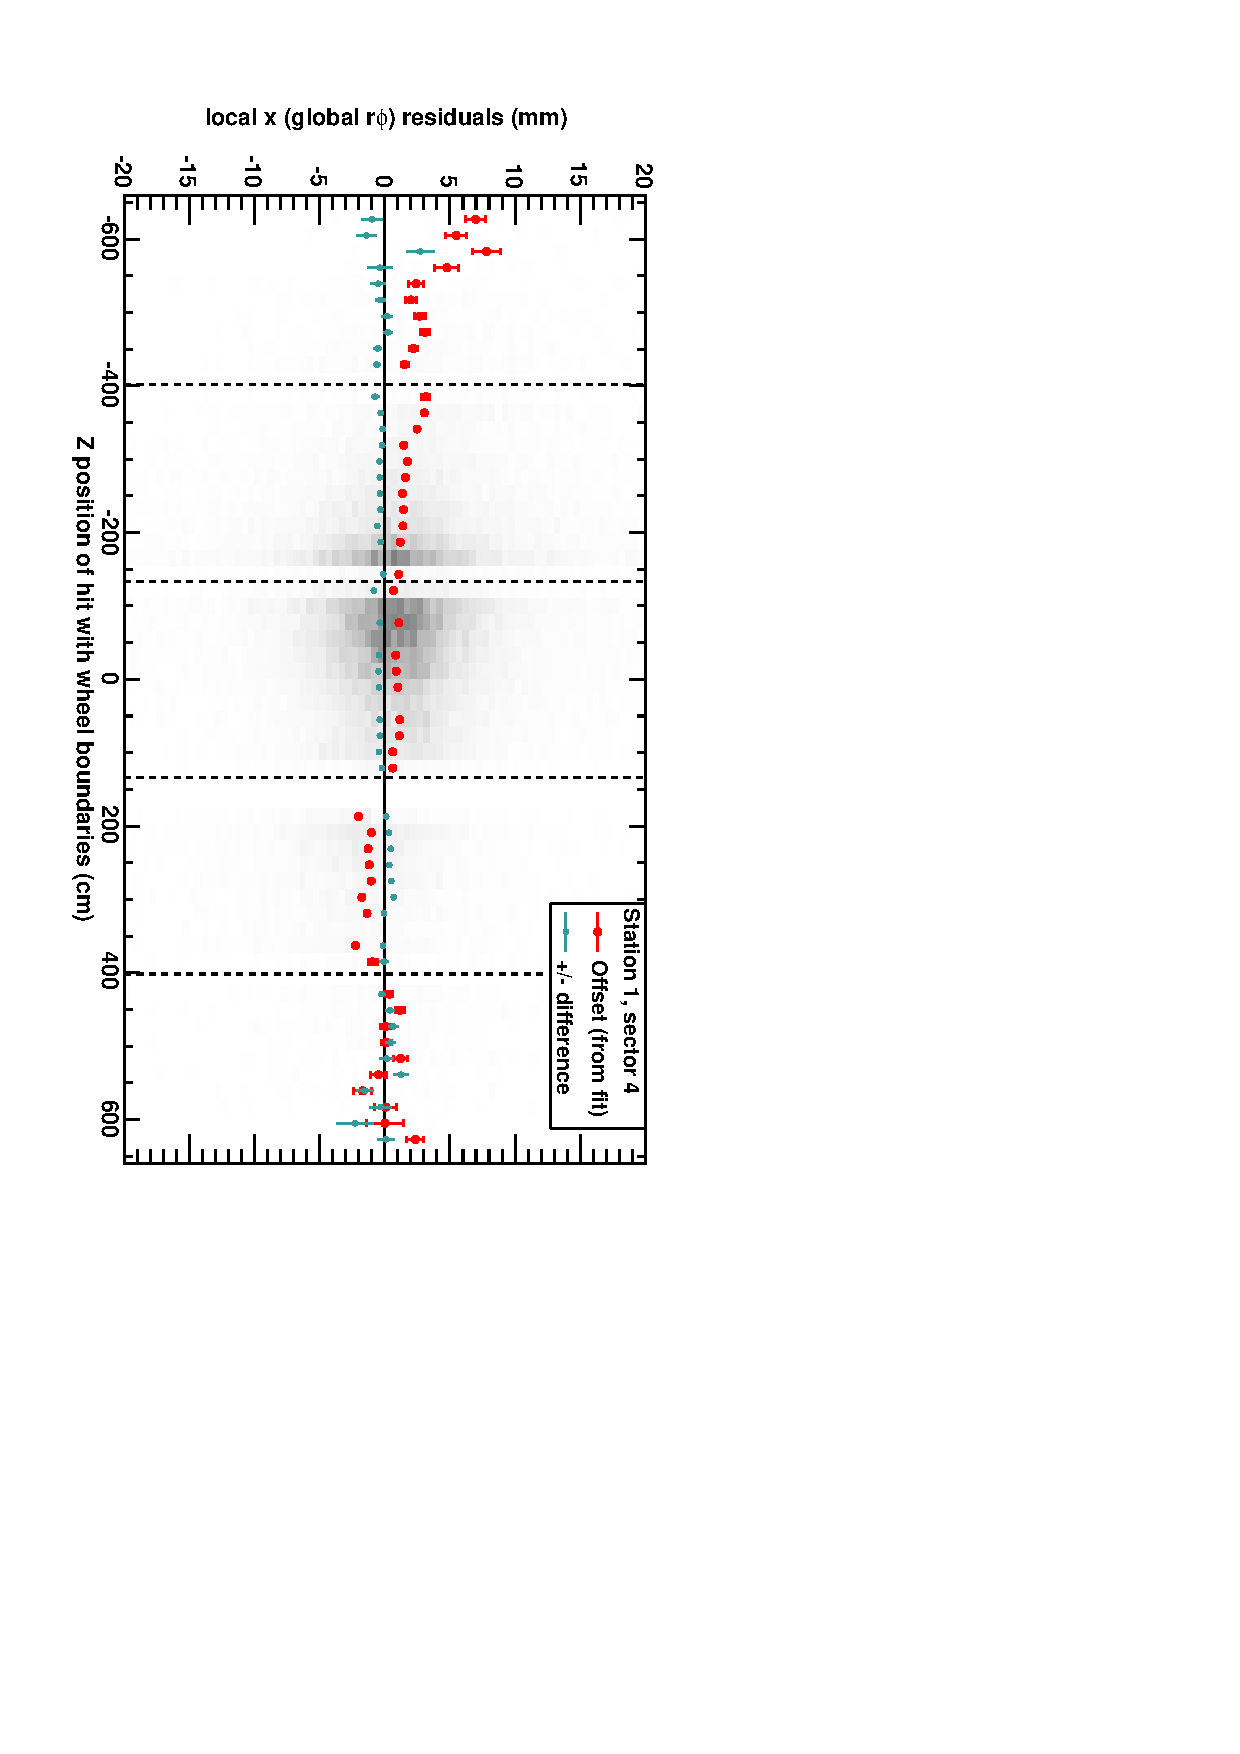
\includegraphics[height=1.2\linewidth, angle=90]{DTrphiVsZ_st1_sr04.pdf}} \end{frame}
\section*{station 1, sector 5}
\begin{frame} \vfill \mbox{\hspace{-1 cm}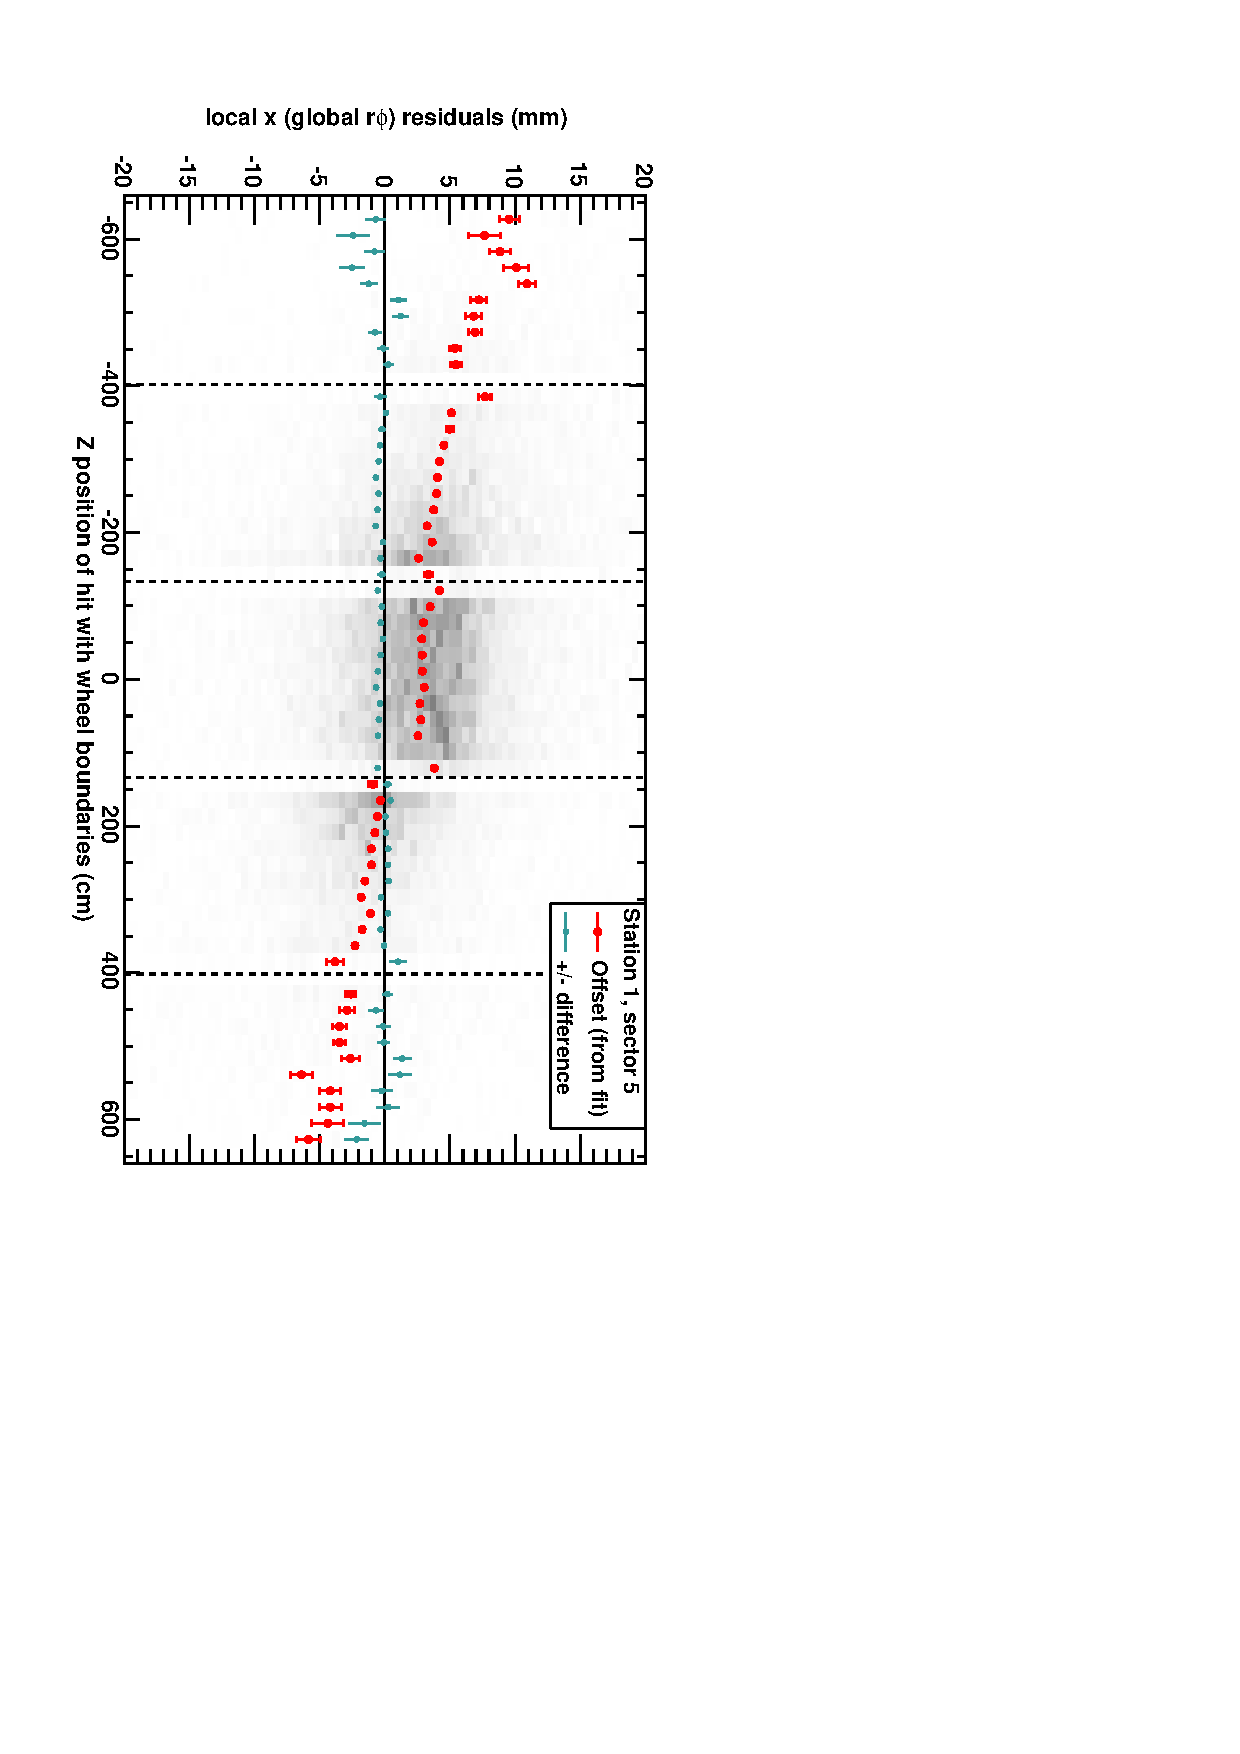
\includegraphics[height=1.2\linewidth, angle=90]{DTrphiVsZ_st1_sr05.pdf}} \end{frame}
\section*{station 1, sector 6}
\begin{frame} \vfill \mbox{\hspace{-1 cm}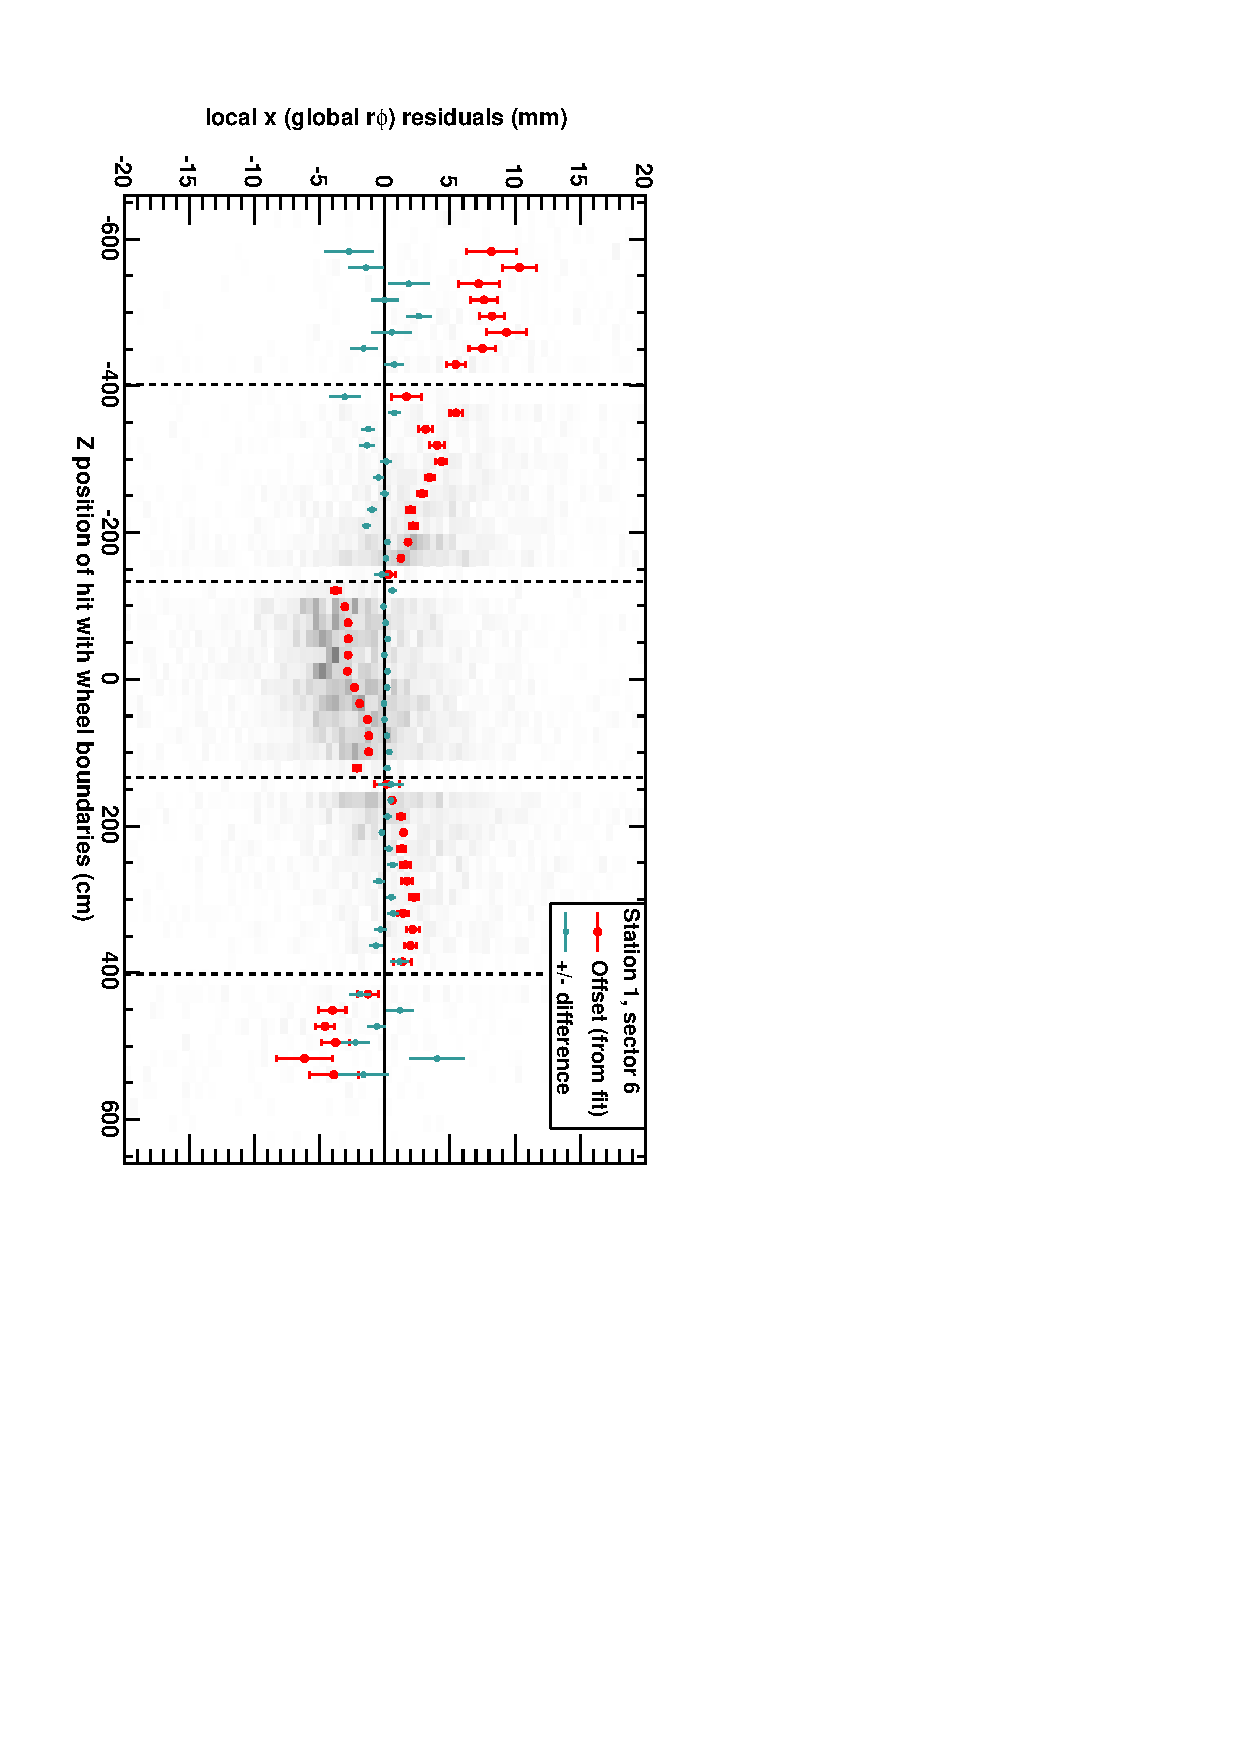
\includegraphics[height=1.2\linewidth, angle=90]{DTrphiVsZ_st1_sr06.pdf}} \end{frame}
\section*{station 1, sector 7}
\begin{frame} \vfill \mbox{\hspace{-1 cm}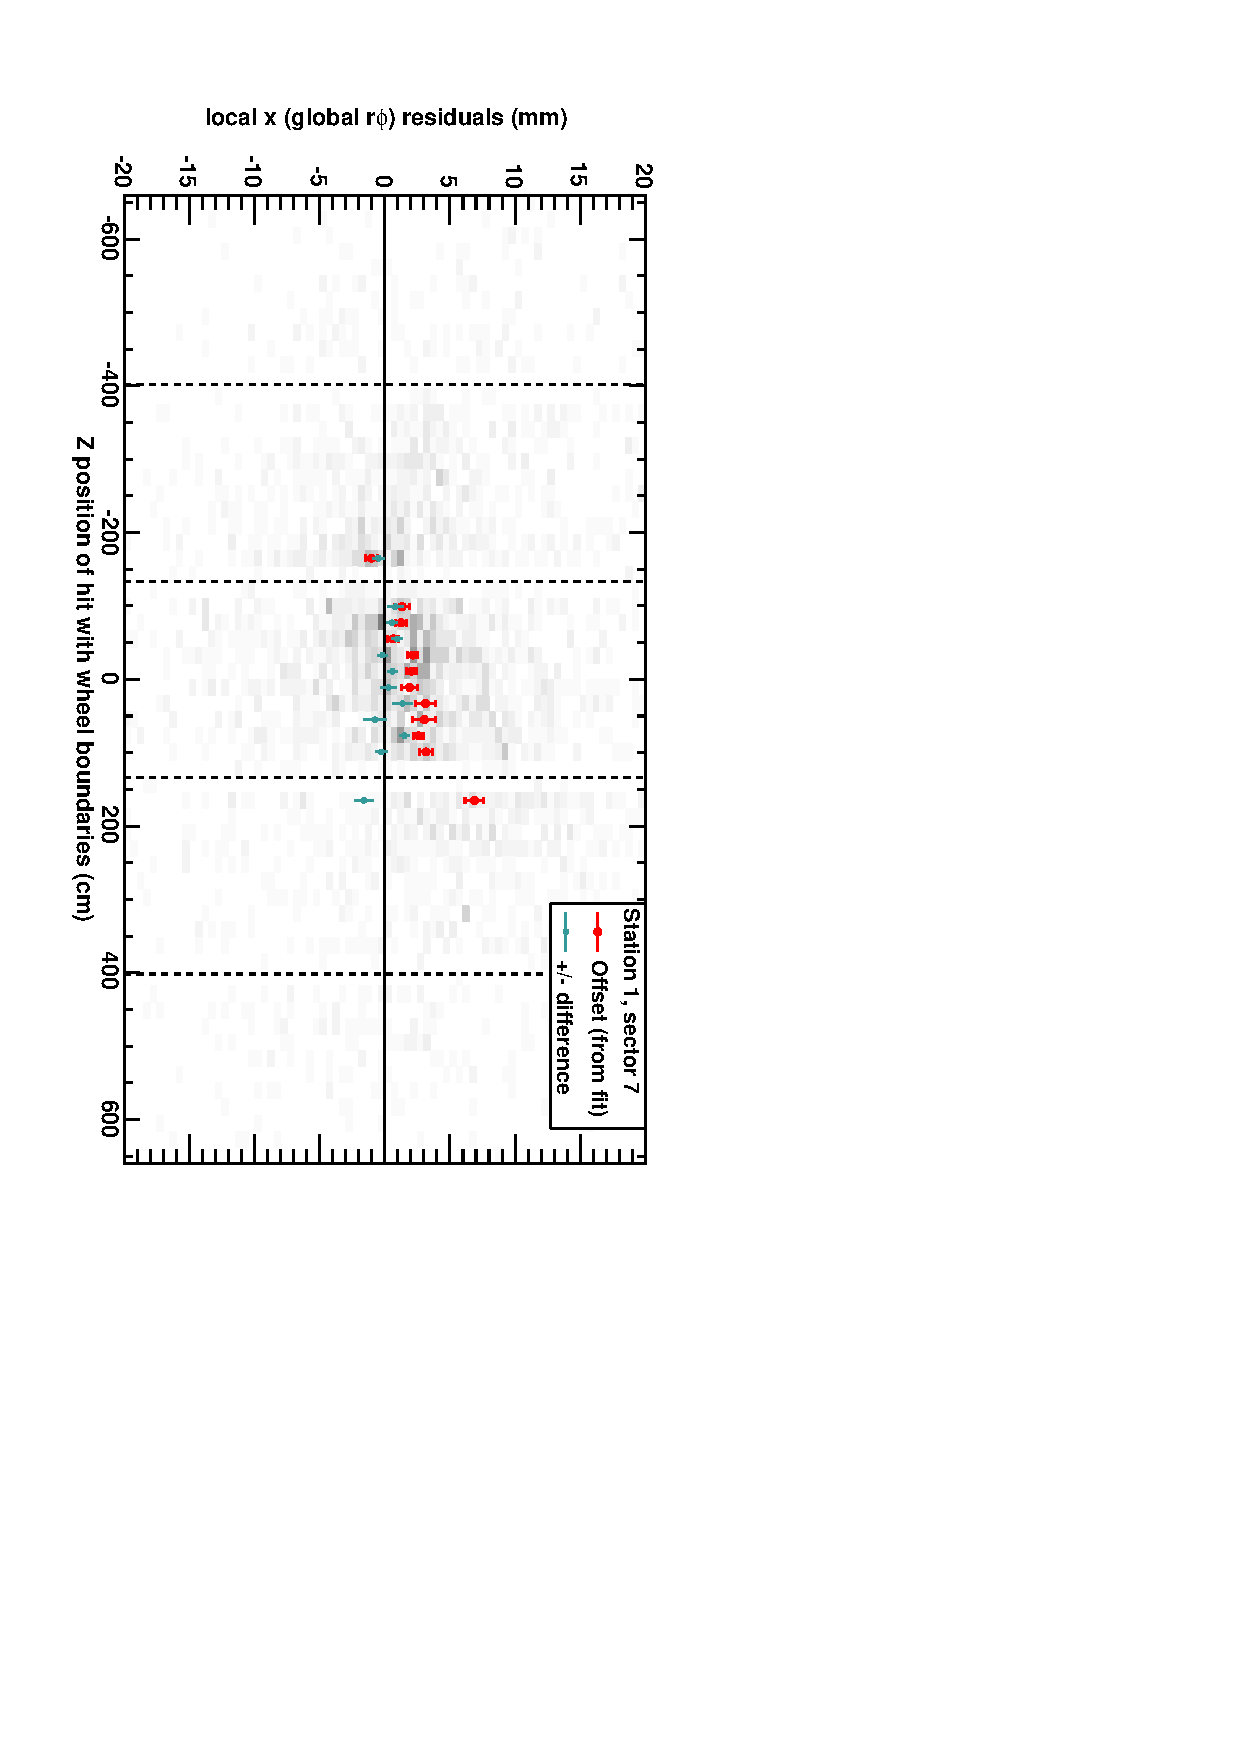
\includegraphics[height=1.2\linewidth, angle=90]{DTrphiVsZ_st1_sr07.pdf}} \end{frame}
\section*{station 1, sector 8}
\begin{frame} \vfill \mbox{\hspace{-1 cm}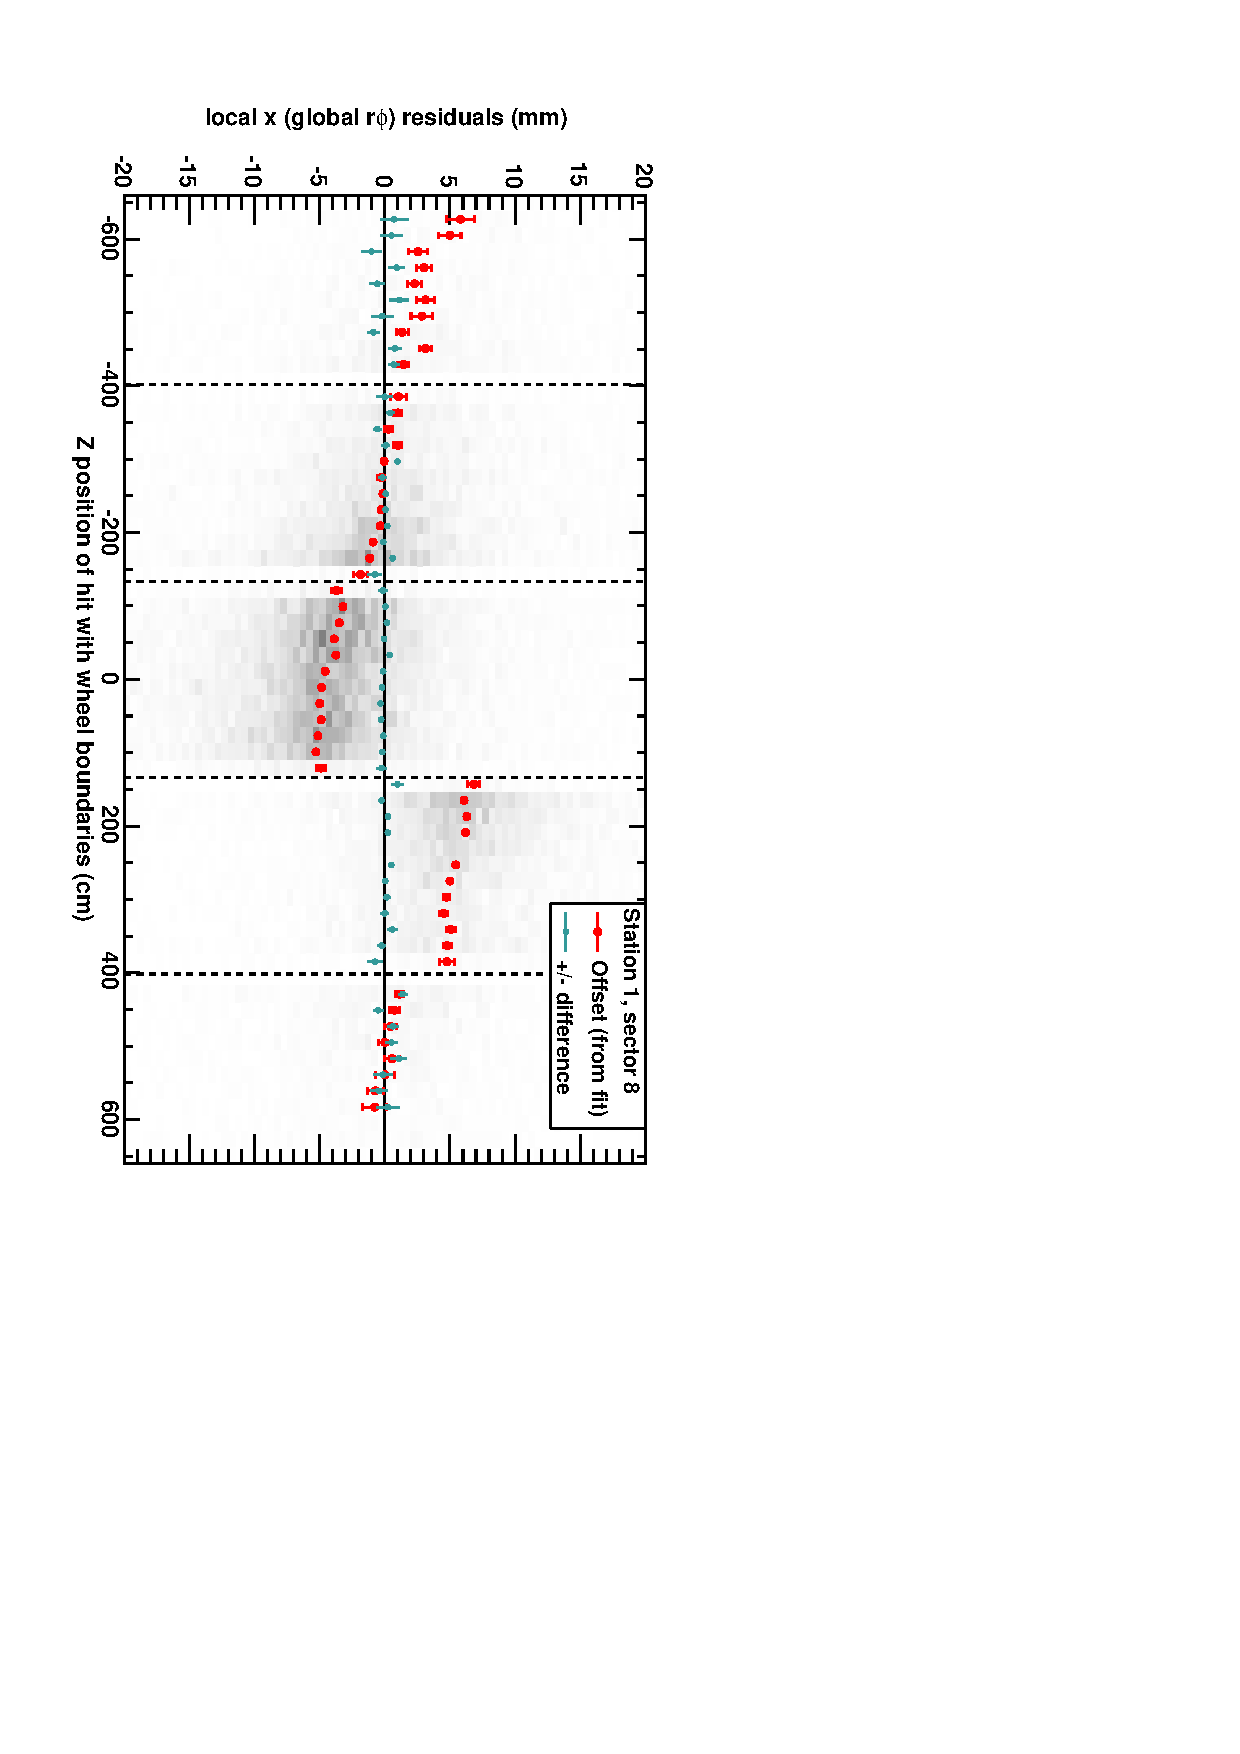
\includegraphics[height=1.2\linewidth, angle=90]{DTrphiVsZ_st1_sr08.pdf}} \end{frame}
\section*{station 1, sector 9}
\begin{frame} \vfill \mbox{\hspace{-1 cm}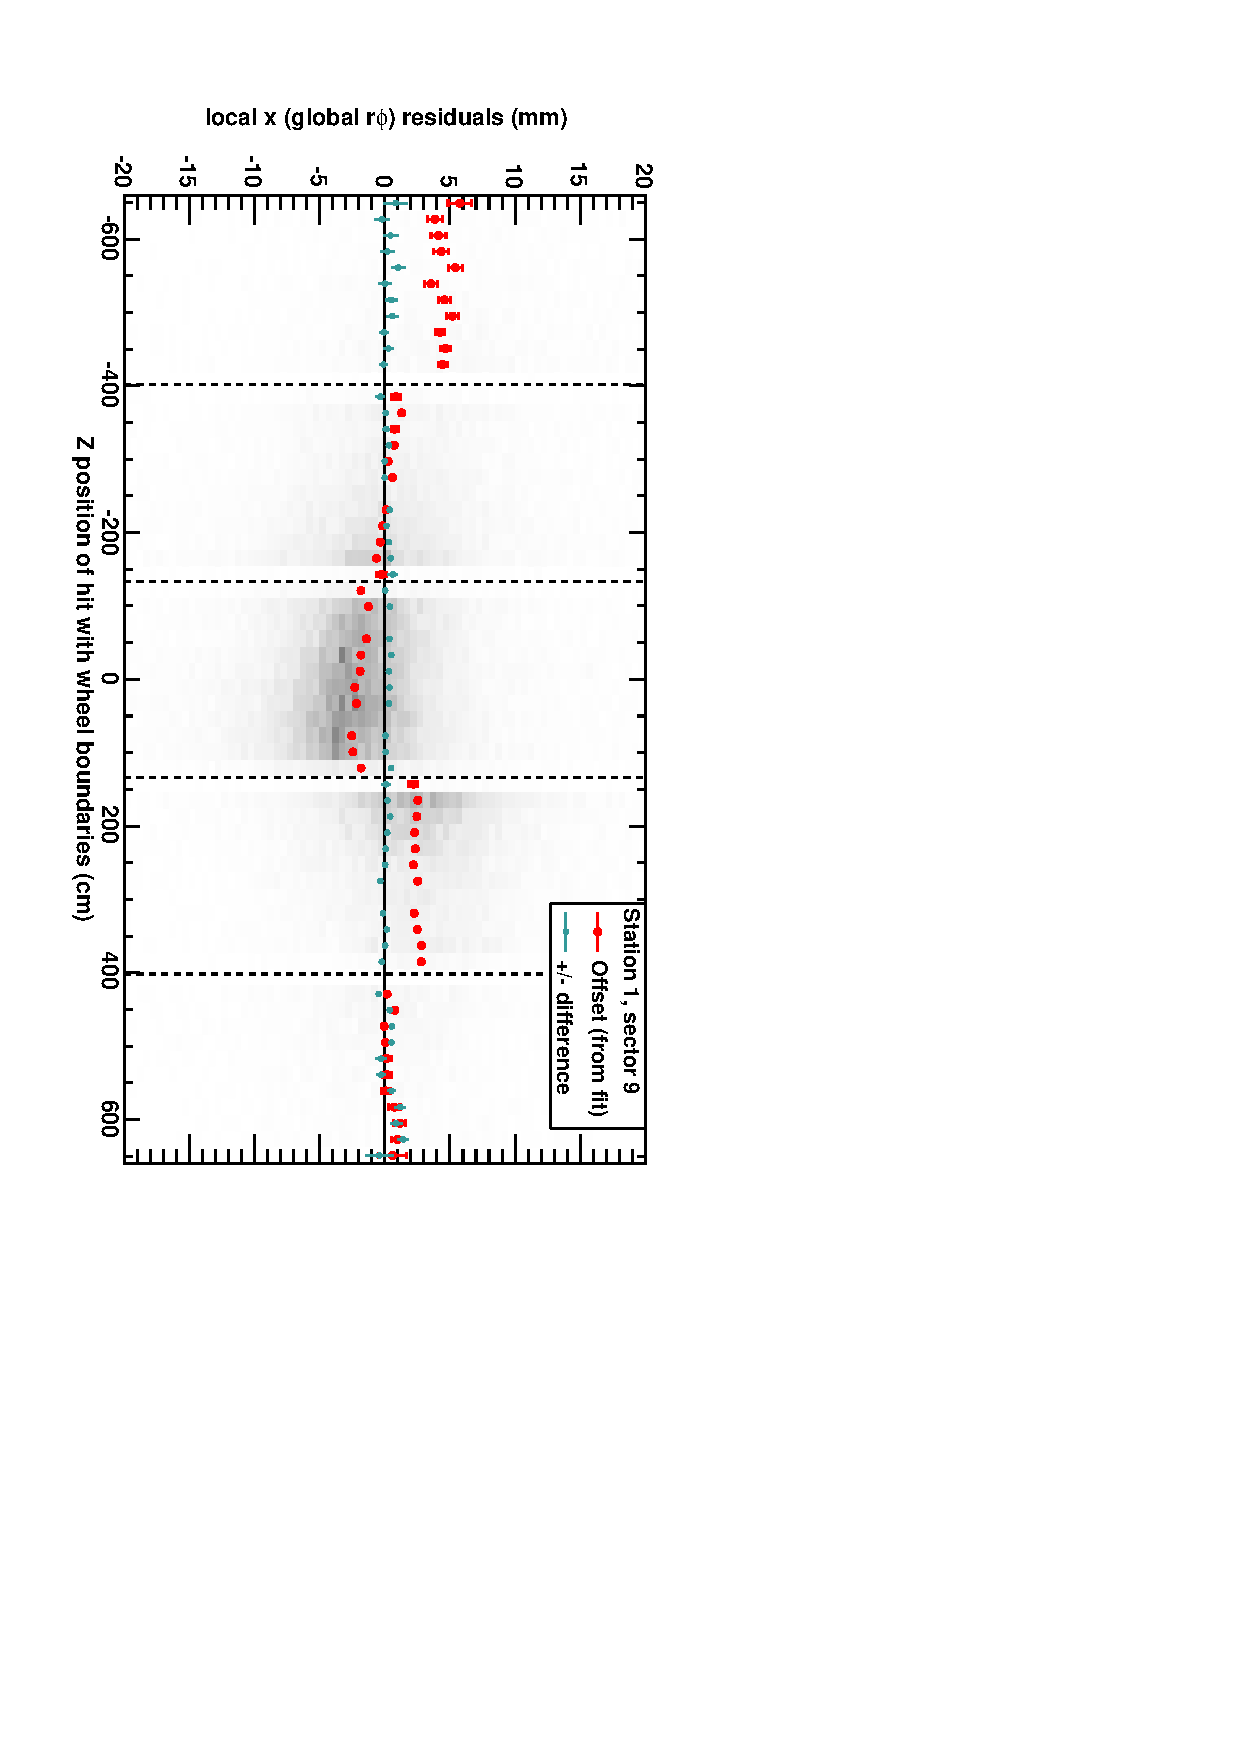
\includegraphics[height=1.2\linewidth, angle=90]{DTrphiVsZ_st1_sr09.pdf}} \end{frame}
\section*{station 1, sector 10}
\begin{frame} \vfill \mbox{\hspace{-1 cm}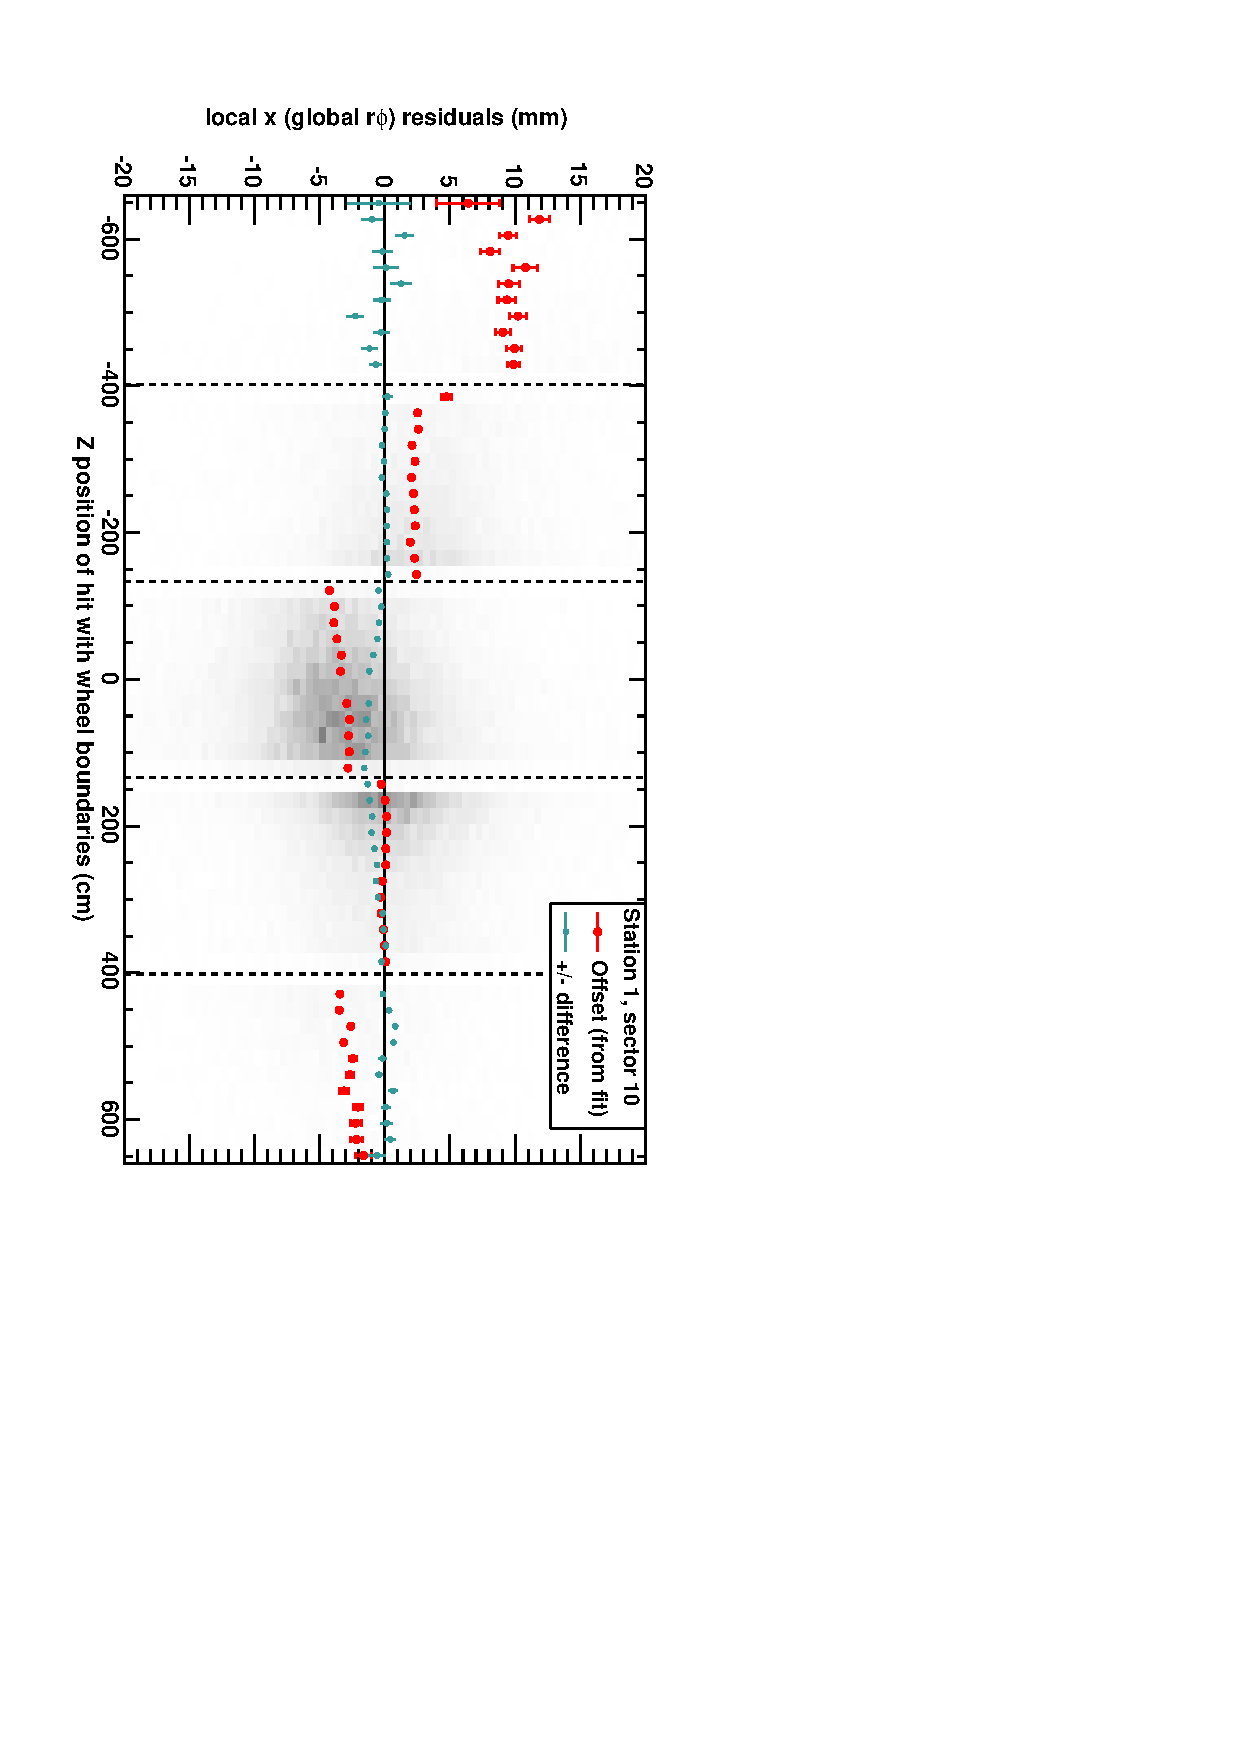
\includegraphics[height=1.2\linewidth, angle=90]{DTrphiVsZ_st1_sr10.pdf}} \end{frame}
\section*{station 1, sector 11}
\begin{frame} \vfill \mbox{\hspace{-1 cm}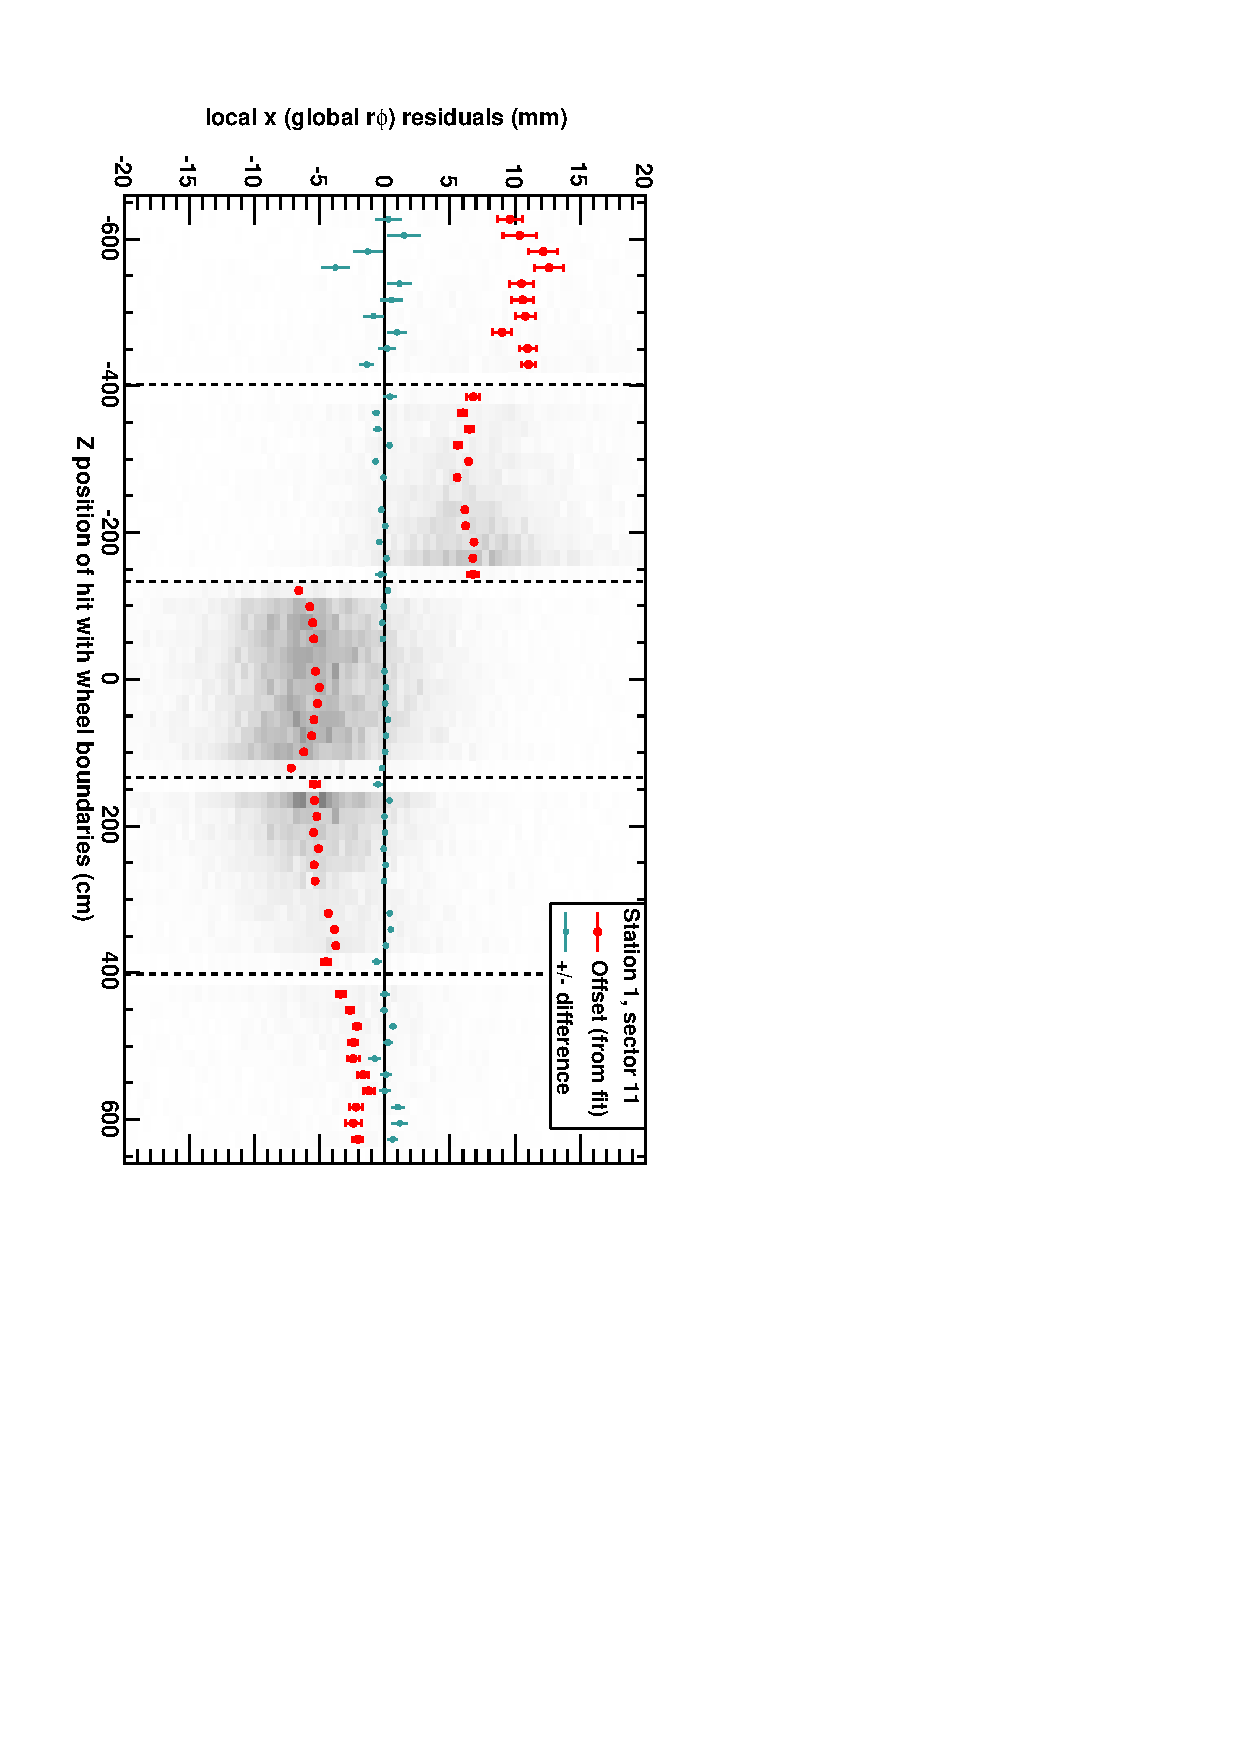
\includegraphics[height=1.2\linewidth, angle=90]{DTrphiVsZ_st1_sr11.pdf}} \end{frame}
\section*{station 1, sector 12}
\begin{frame} \vfill \mbox{\hspace{-1 cm}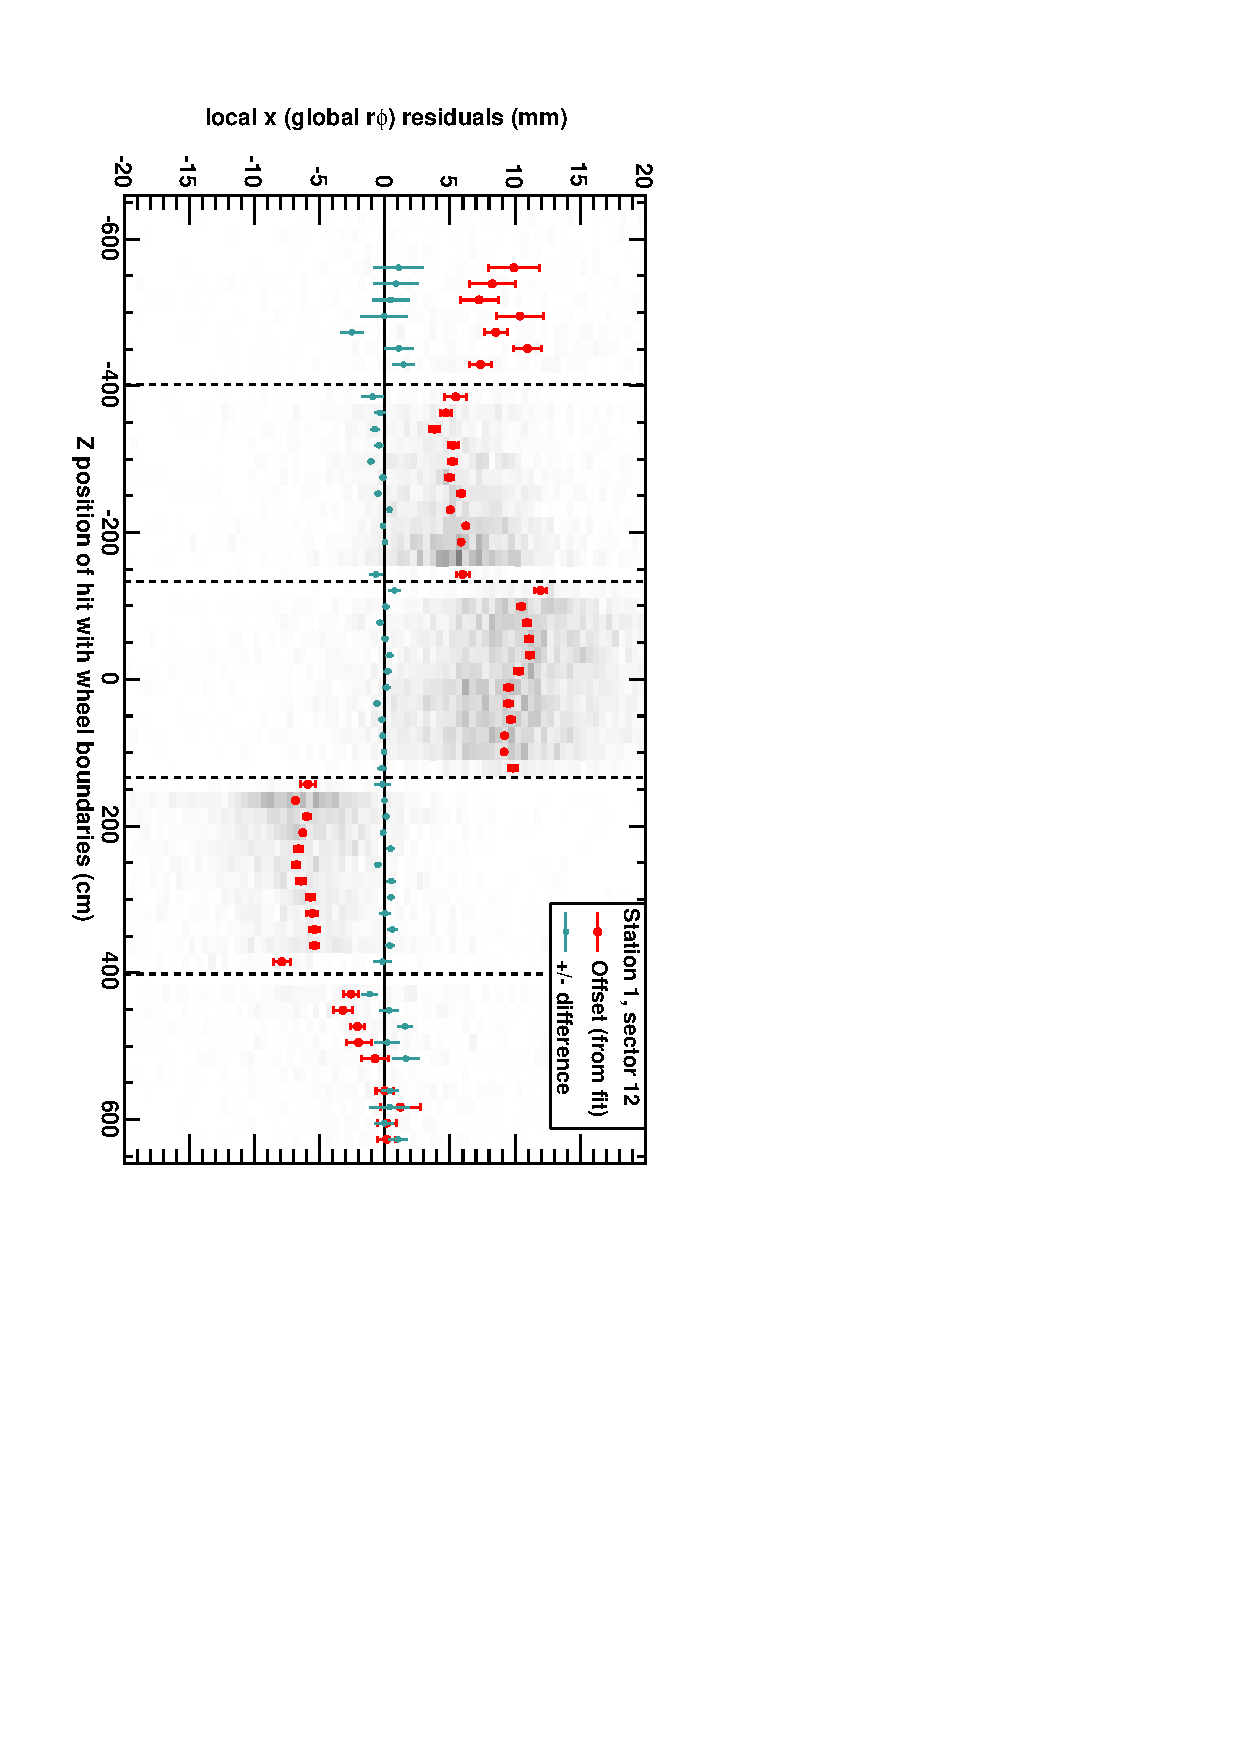
\includegraphics[height=1.2\linewidth, angle=90]{DTrphiVsZ_st1_sr12.pdf}} \end{frame}
\section*{station 2, sector 1}
\begin{frame} \vfill \mbox{\hspace{-1 cm}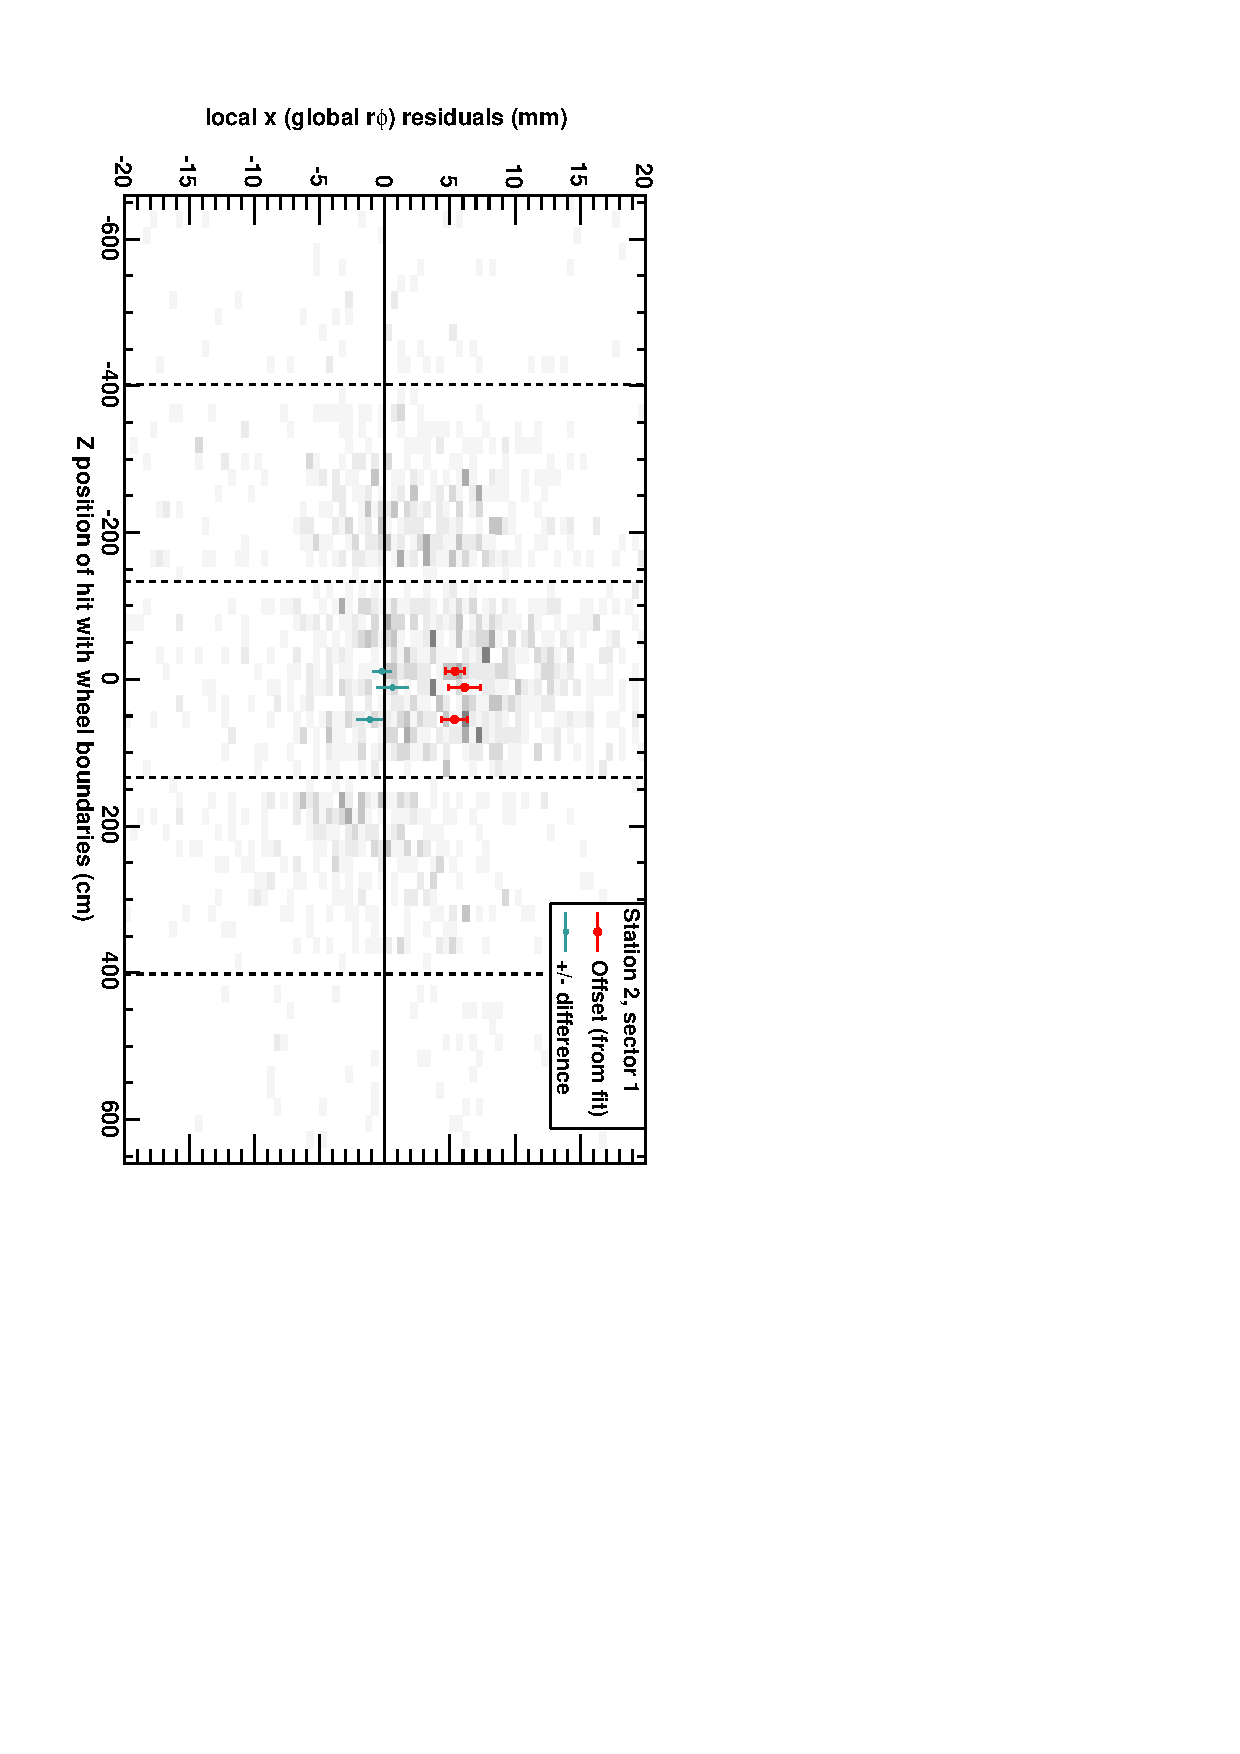
\includegraphics[height=1.2\linewidth, angle=90]{DTrphiVsZ_st2_sr01.pdf}} \end{frame}
\section*{station 2, sector 2}
\begin{frame} \vfill \mbox{\hspace{-1 cm}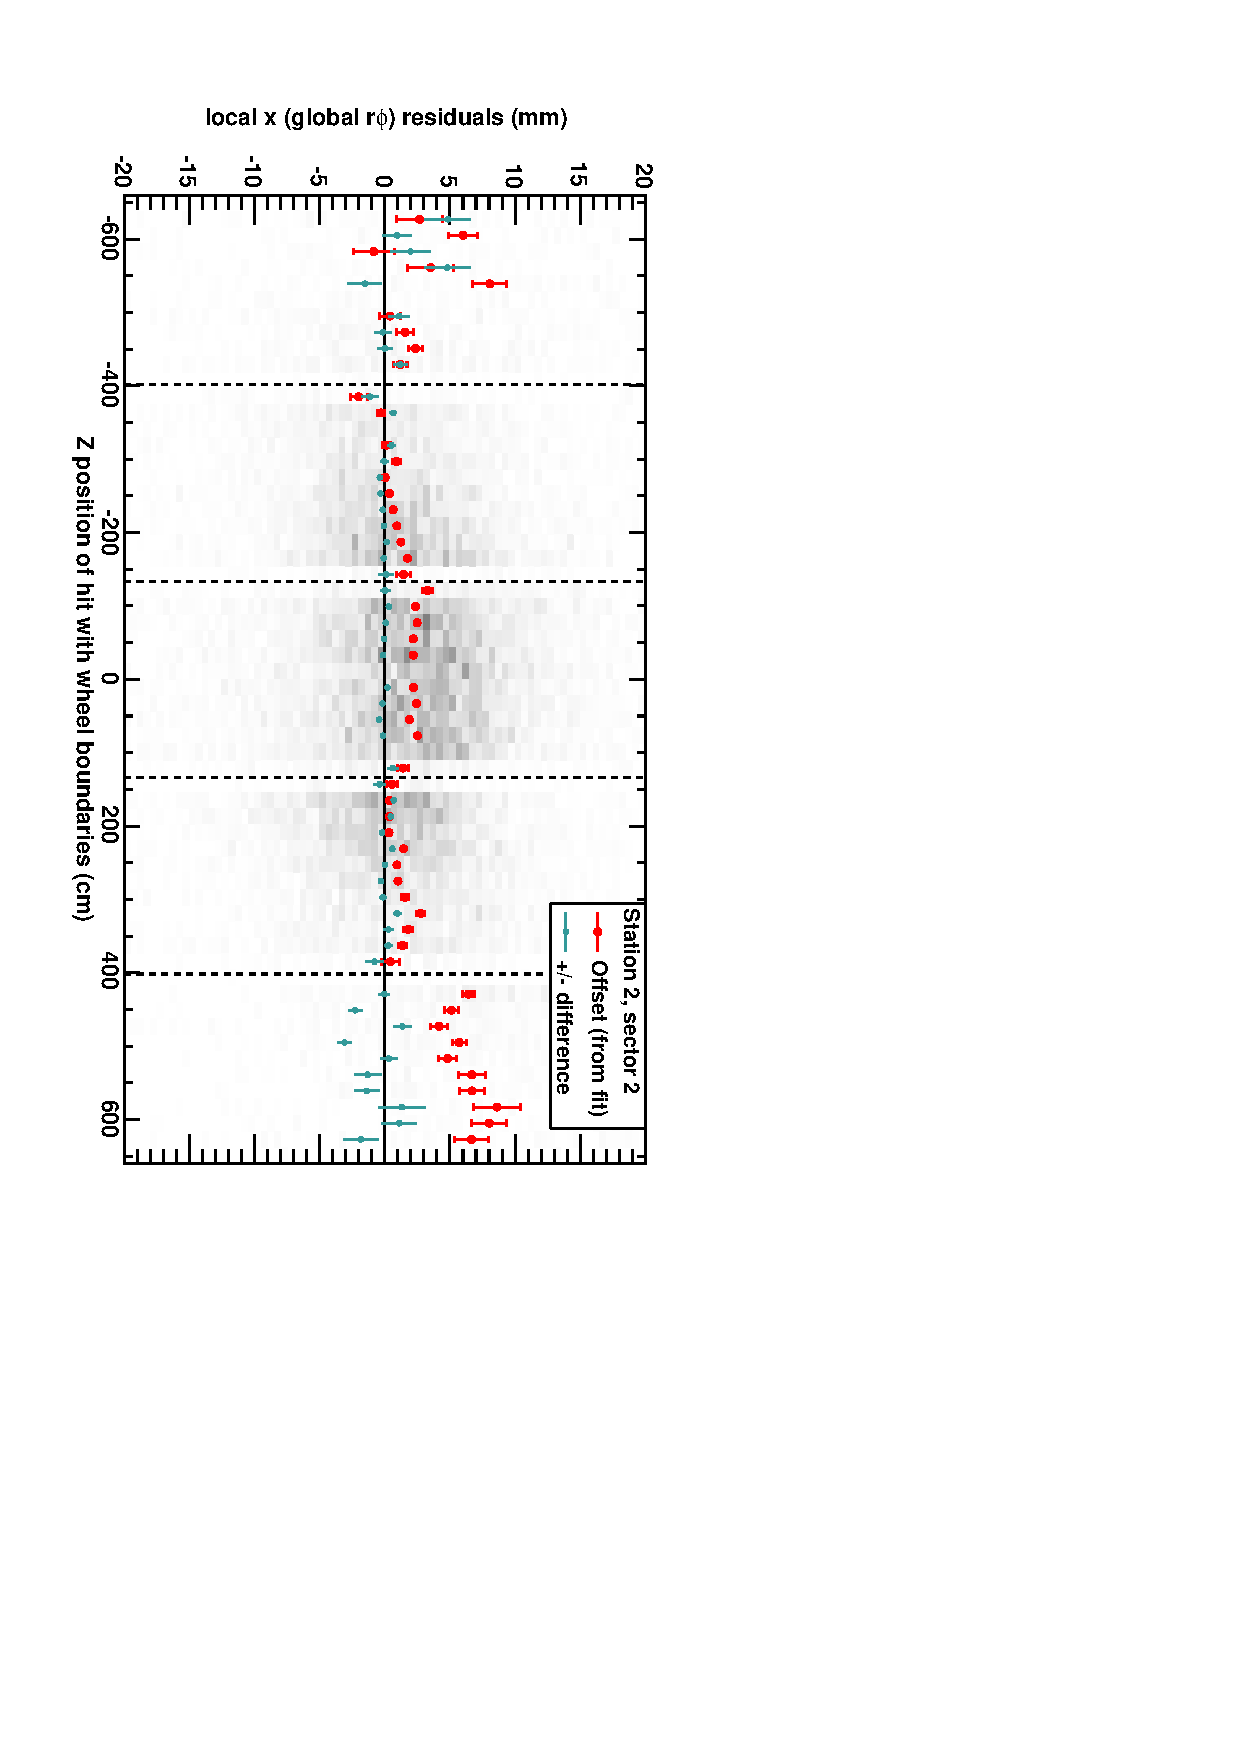
\includegraphics[height=1.2\linewidth, angle=90]{DTrphiVsZ_st2_sr02.pdf}} \end{frame}
\section*{station 2, sector 3}
\begin{frame} \vfill \mbox{\hspace{-1 cm}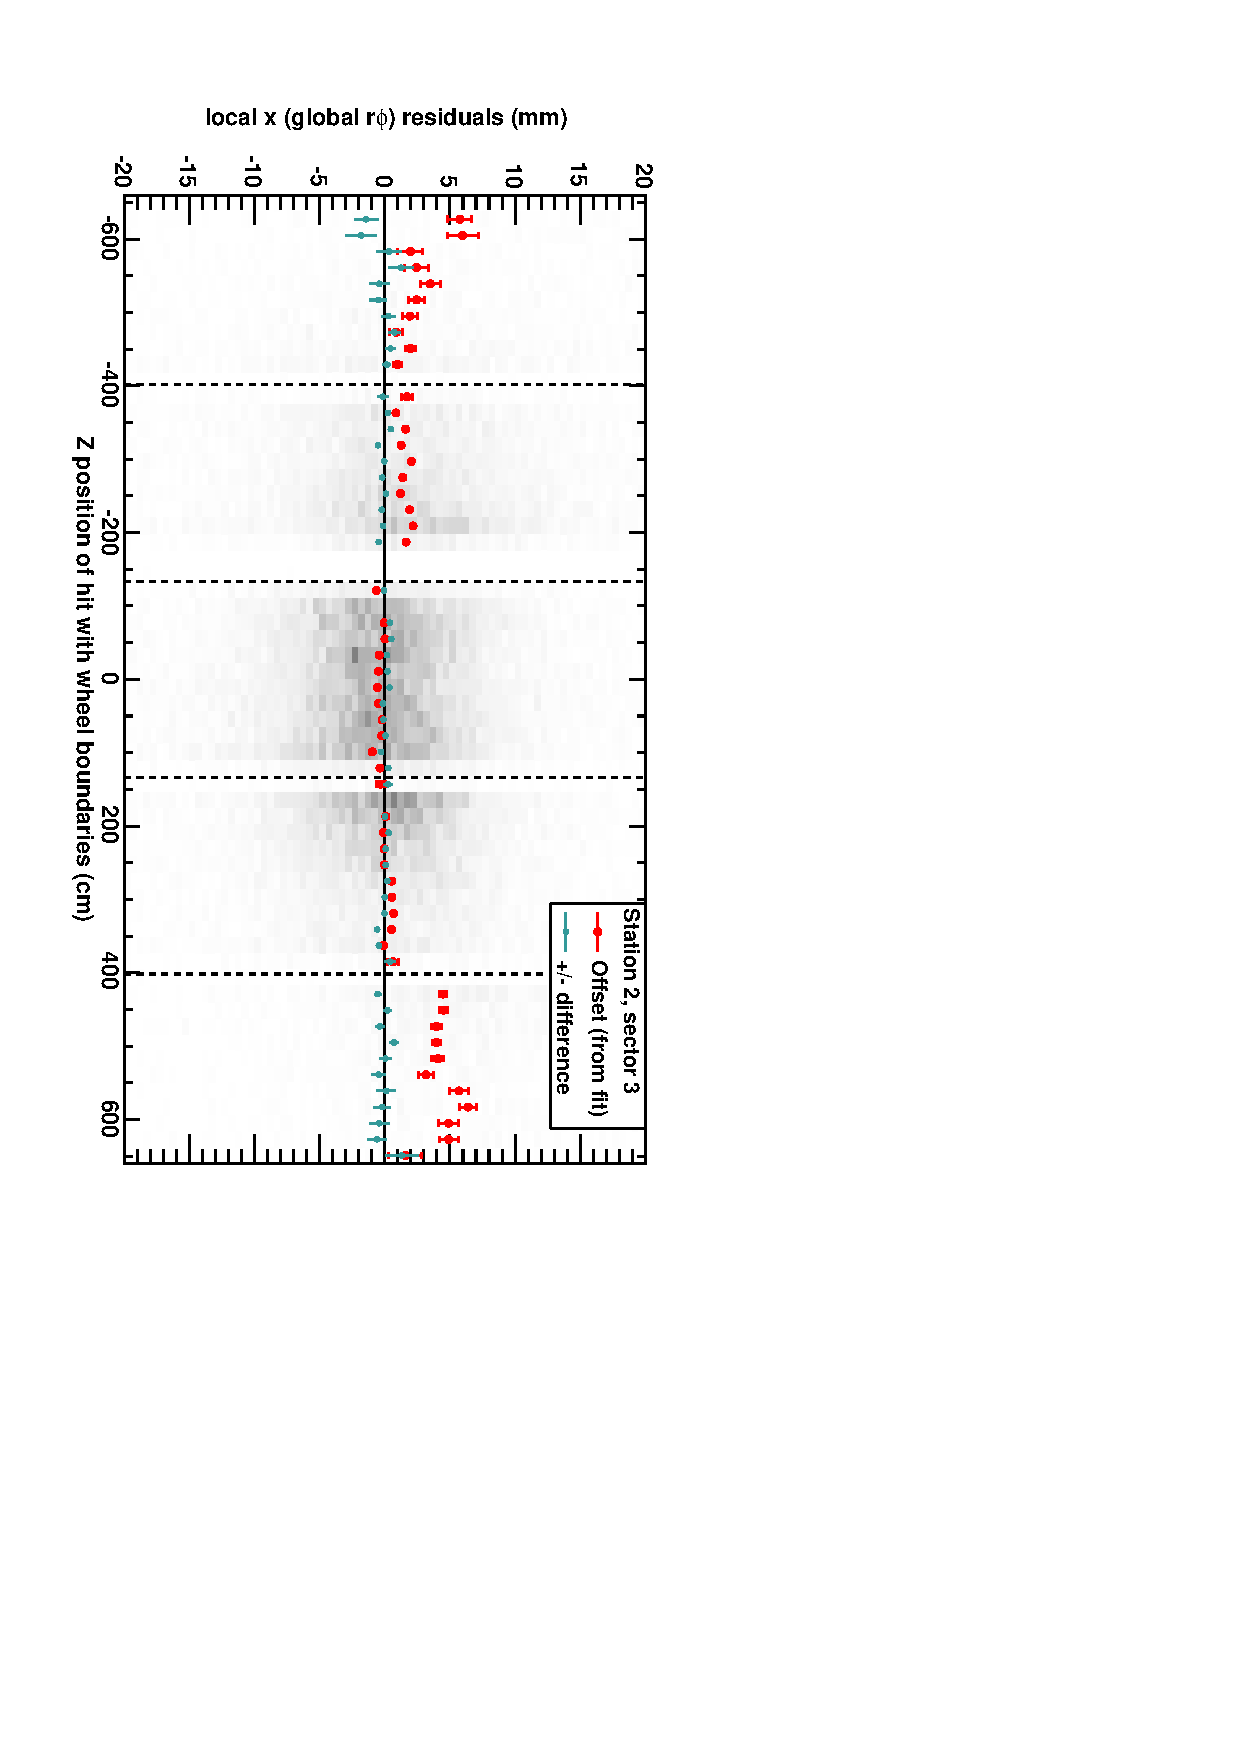
\includegraphics[height=1.2\linewidth, angle=90]{DTrphiVsZ_st2_sr03.pdf}} \end{frame}
\section*{station 2, sector 4}
\begin{frame} \vfill \mbox{\hspace{-1 cm}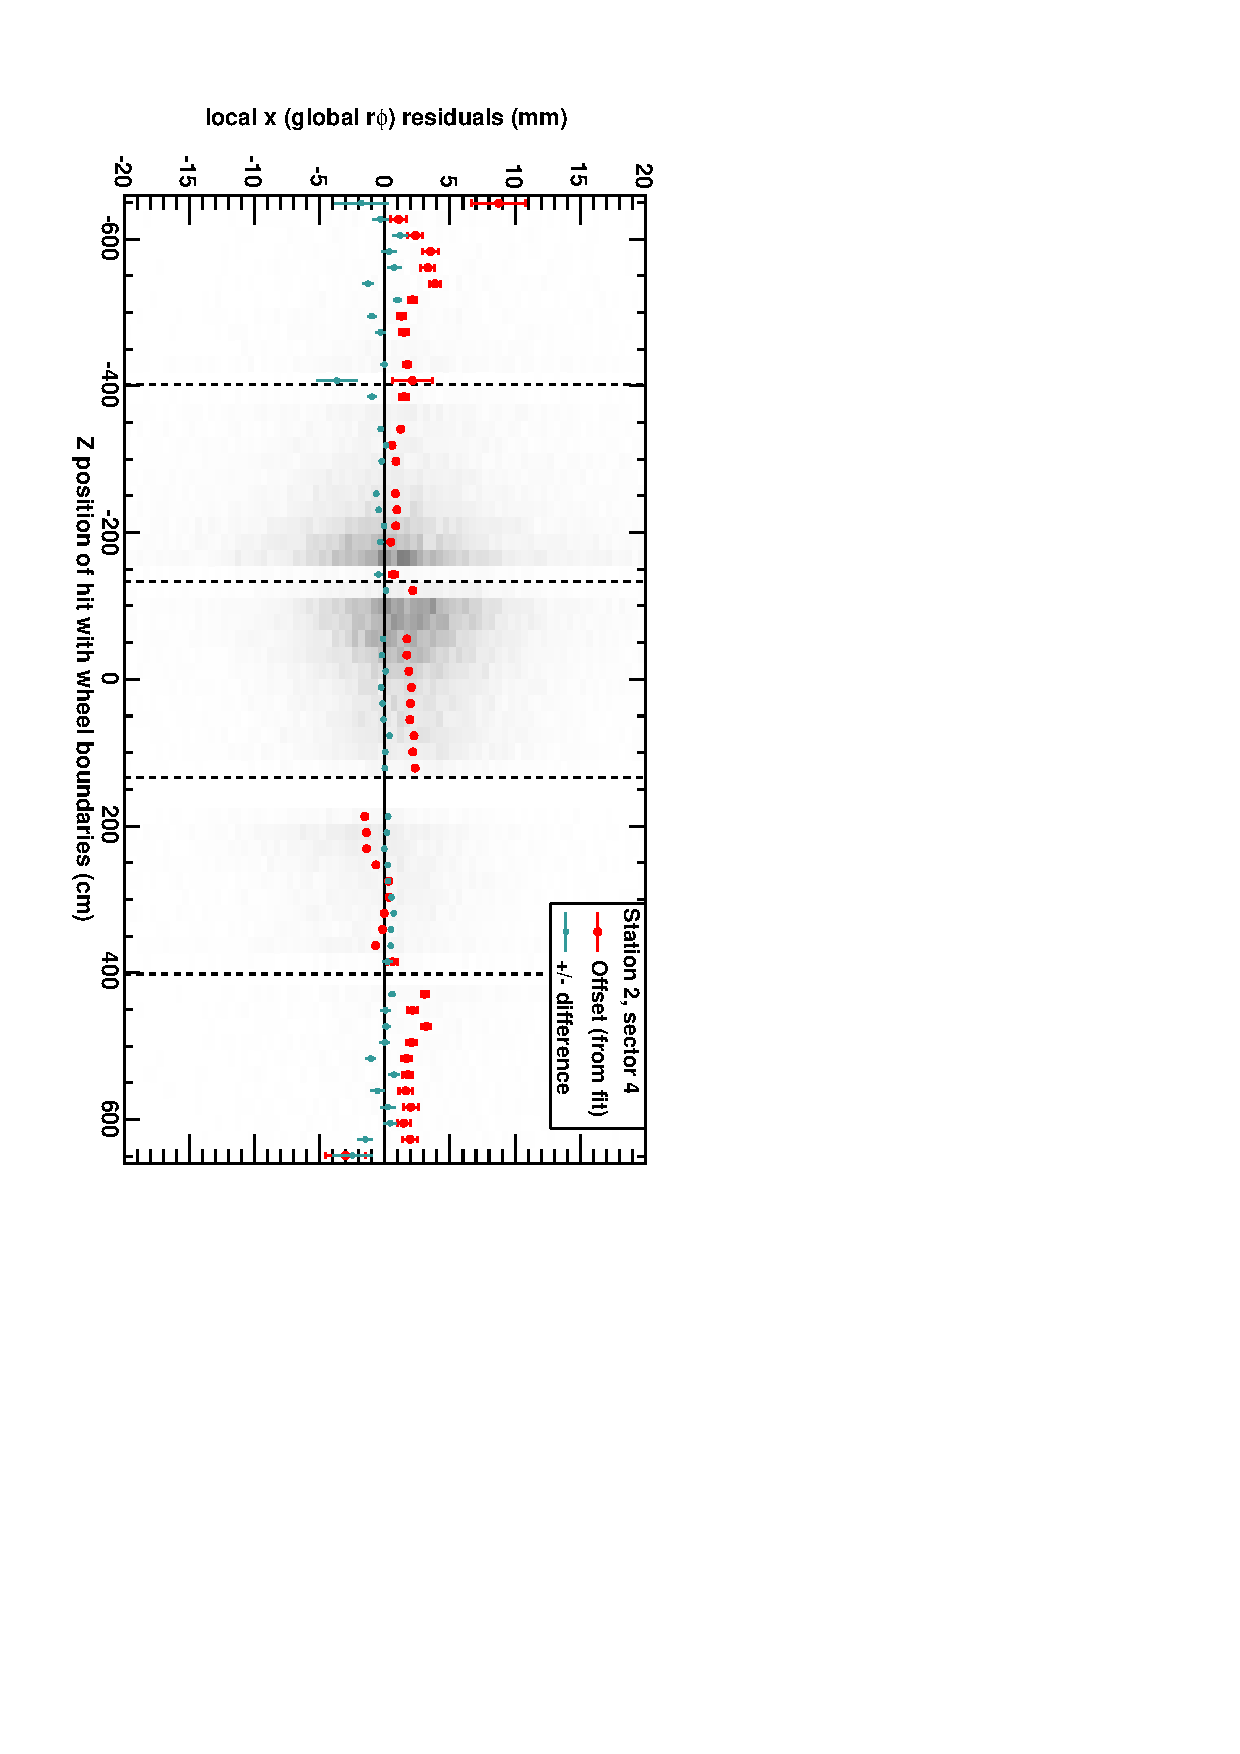
\includegraphics[height=1.2\linewidth, angle=90]{DTrphiVsZ_st2_sr04.pdf}} \end{frame}
\section*{station 2, sector 5}
\begin{frame} \vfill \mbox{\hspace{-1 cm}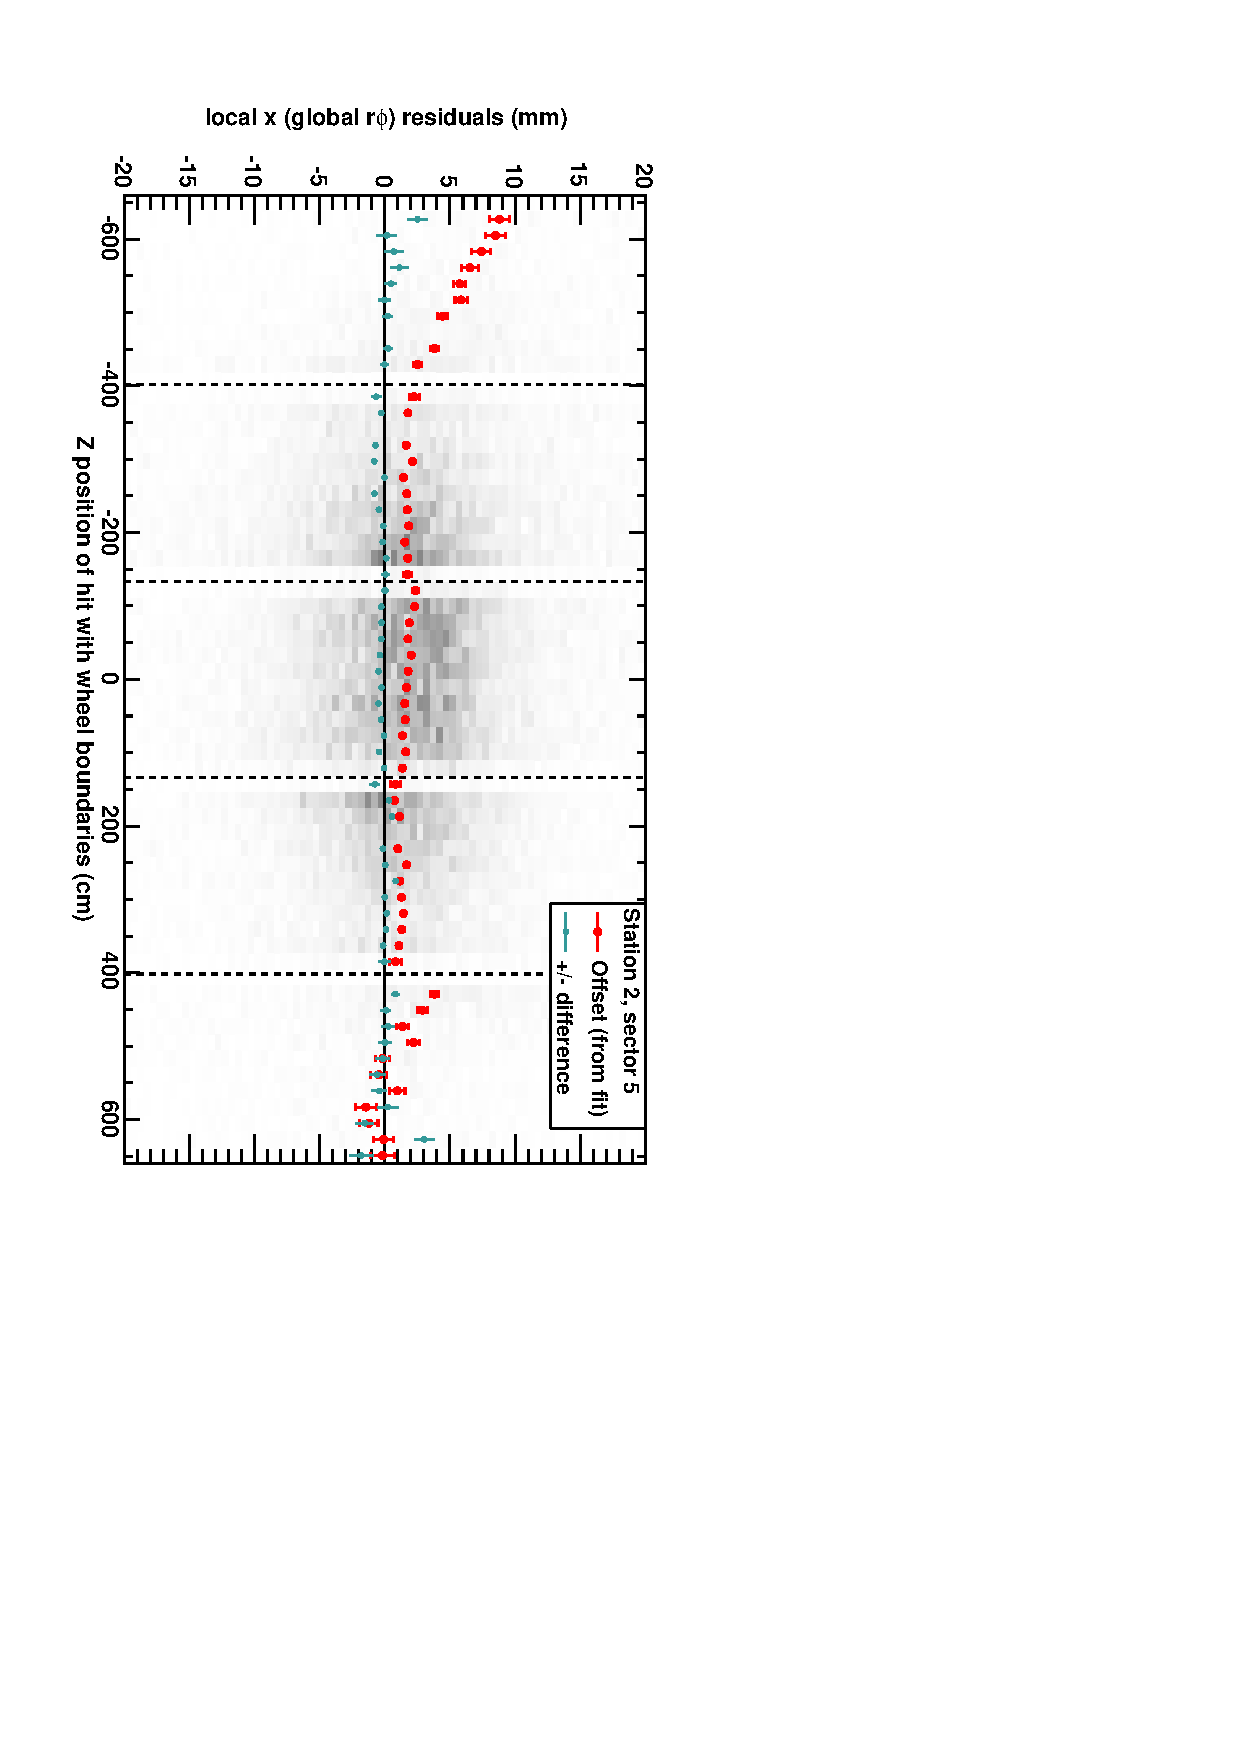
\includegraphics[height=1.2\linewidth, angle=90]{DTrphiVsZ_st2_sr05.pdf}} \end{frame}
\section*{station 2, sector 6}
\begin{frame} \vfill \mbox{\hspace{-1 cm}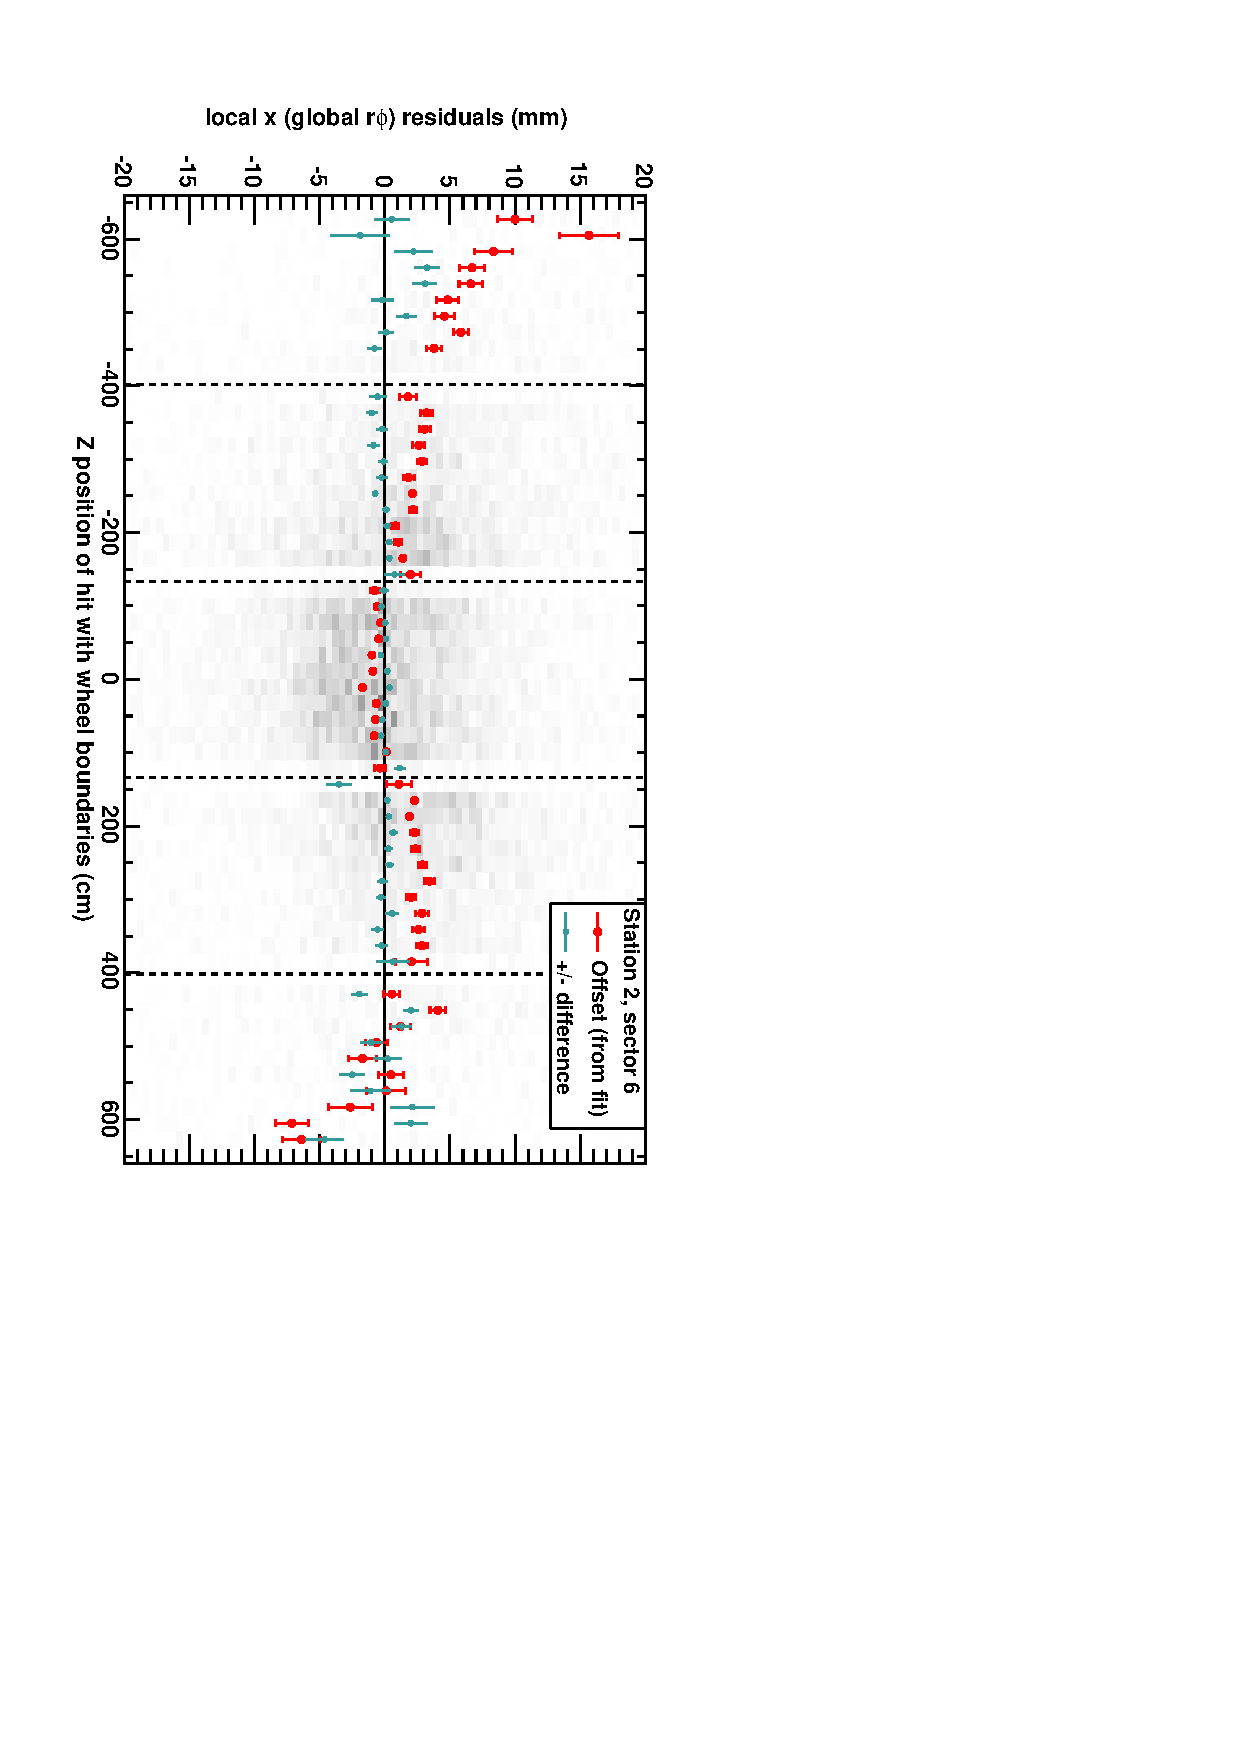
\includegraphics[height=1.2\linewidth, angle=90]{DTrphiVsZ_st2_sr06.pdf}} \end{frame}
\section*{station 2, sector 7}
\begin{frame} \vfill \mbox{\hspace{-1 cm}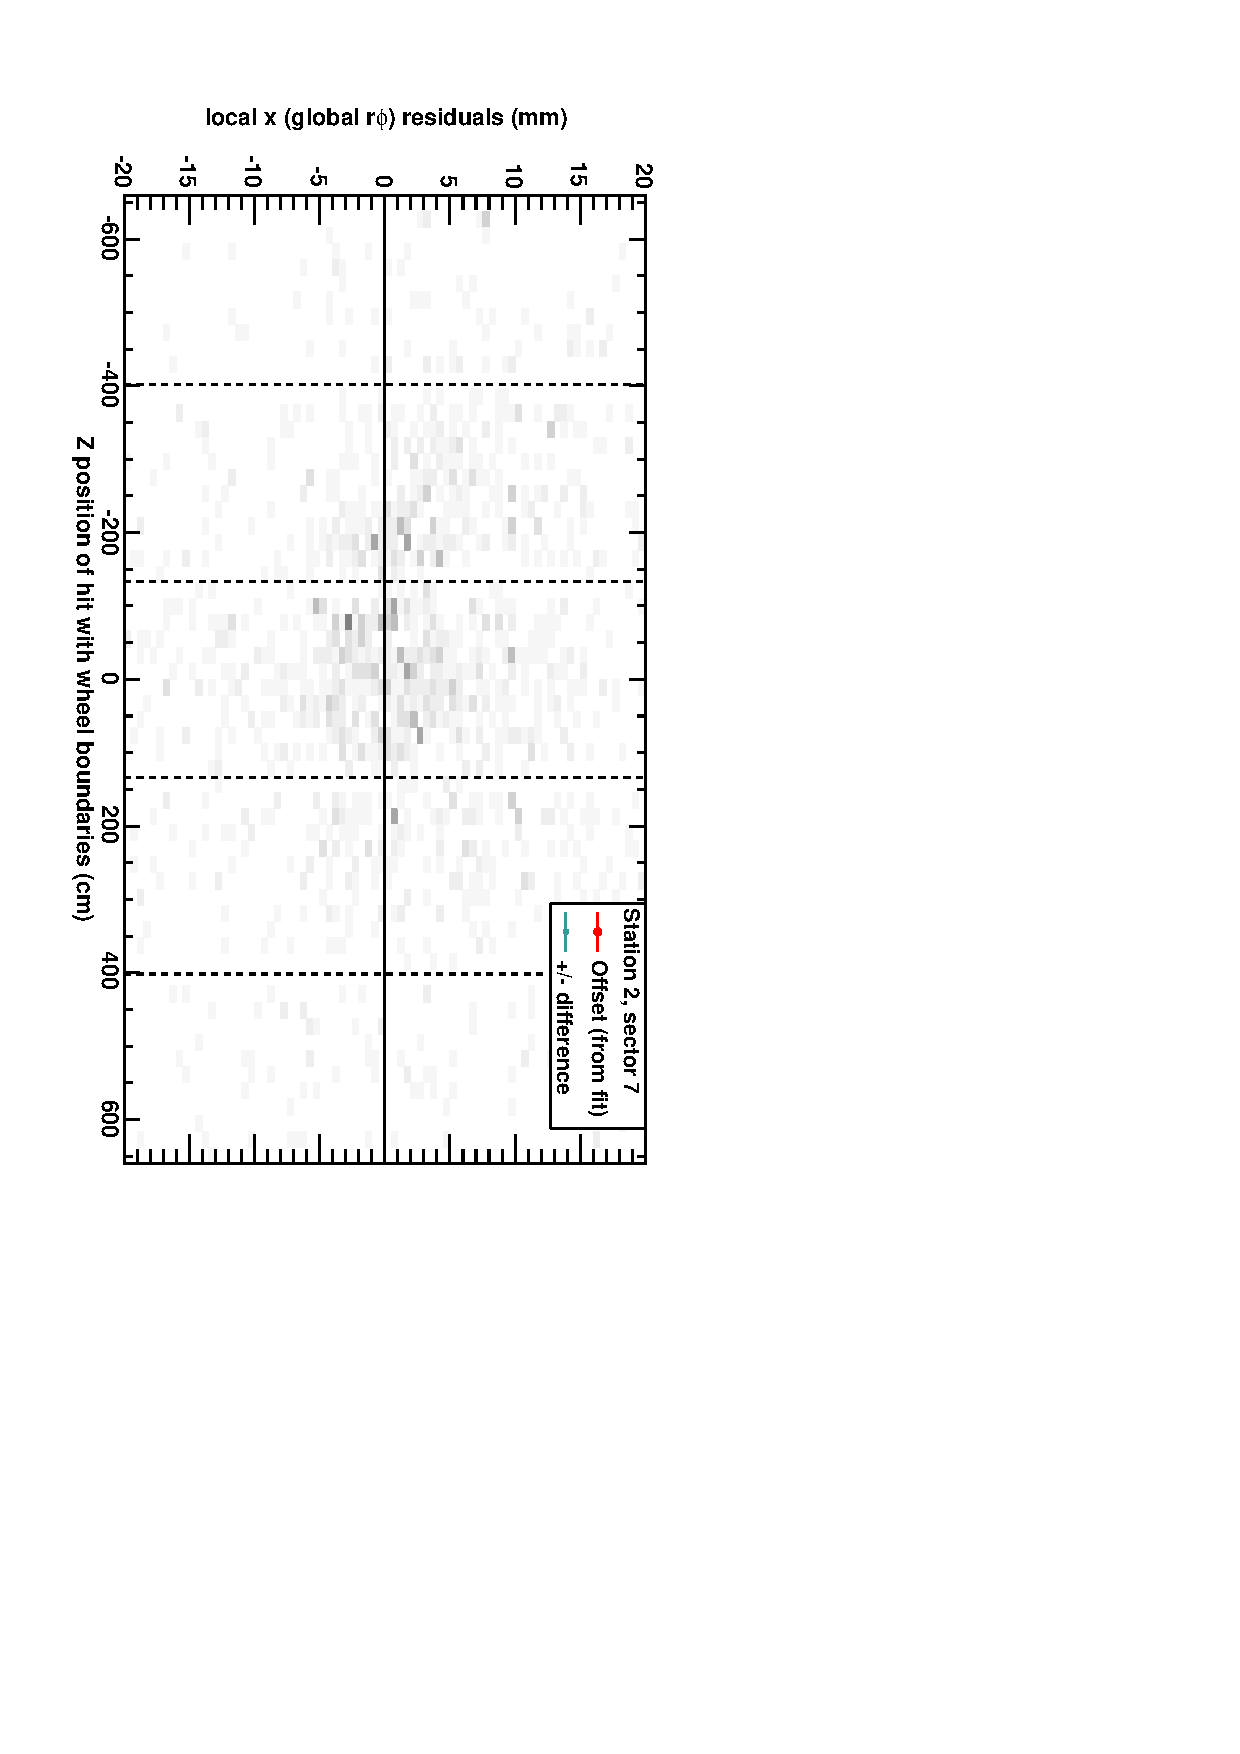
\includegraphics[height=1.2\linewidth, angle=90]{DTrphiVsZ_st2_sr07.pdf}} \end{frame}
\section*{station 2, sector 8}
\begin{frame} \vfill \mbox{\hspace{-1 cm}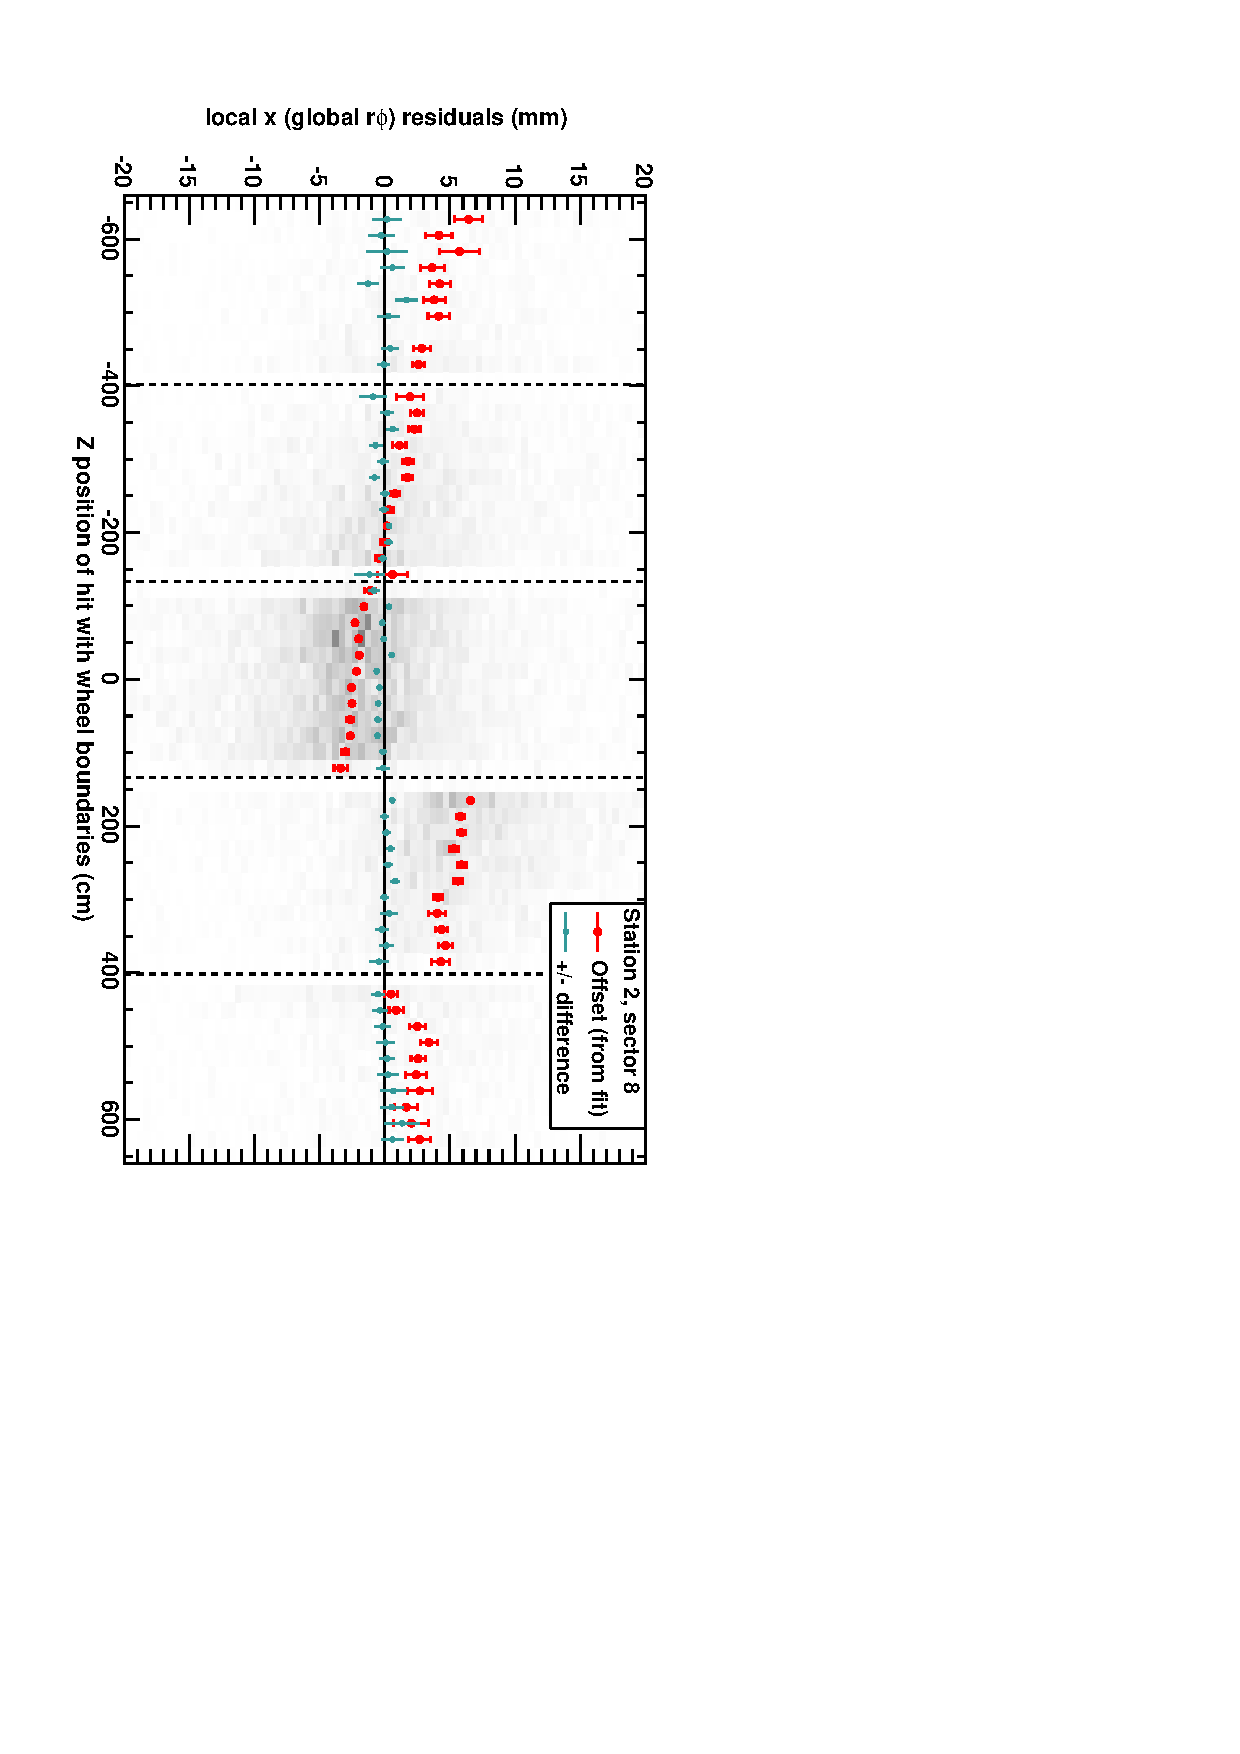
\includegraphics[height=1.2\linewidth, angle=90]{DTrphiVsZ_st2_sr08.pdf}} \end{frame}
\section*{station 2, sector 9}
\begin{frame} \vfill \mbox{\hspace{-1 cm}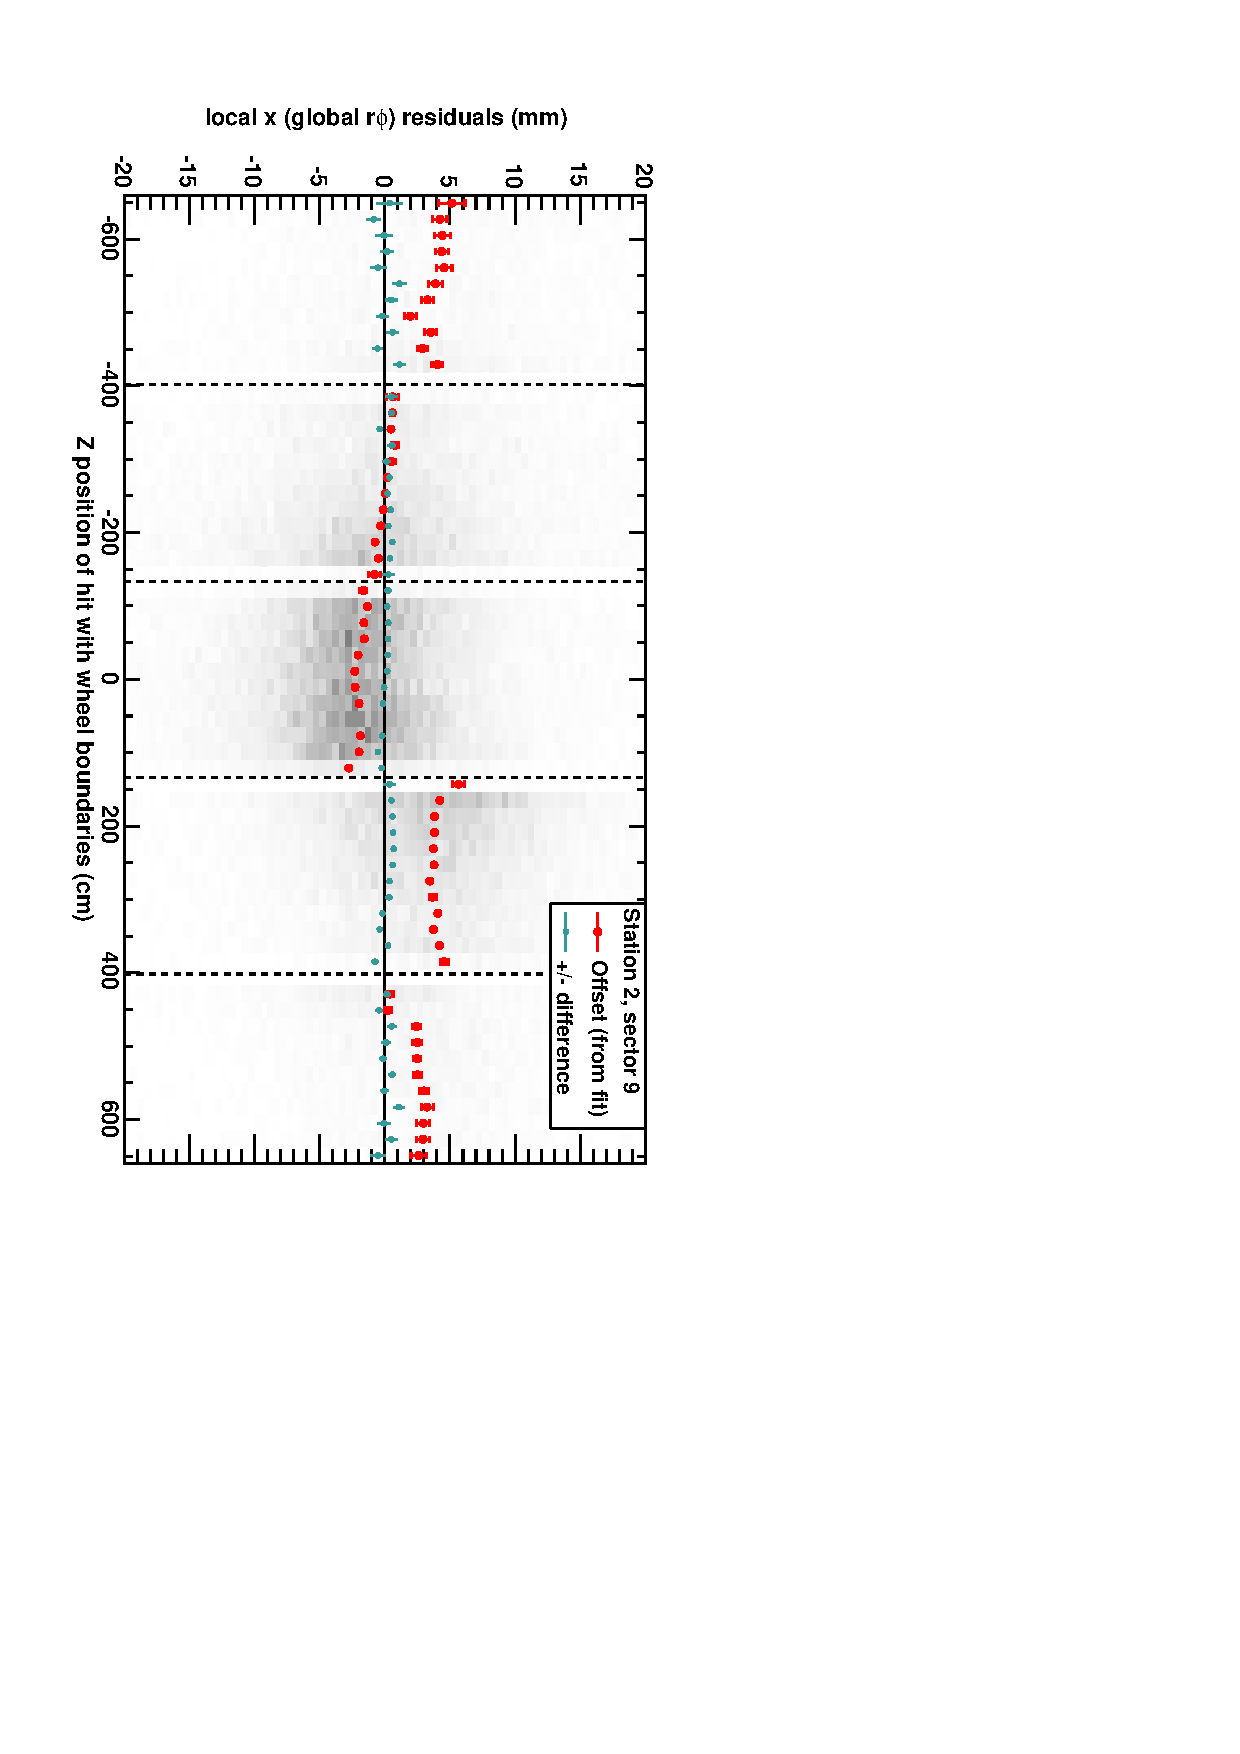
\includegraphics[height=1.2\linewidth, angle=90]{DTrphiVsZ_st2_sr09.pdf}} \end{frame}
\section*{station 2, sector 10}
\begin{frame} \vfill \mbox{\hspace{-1 cm}\includegraphics[height=1.2\linewidth, angle=90]{DTrphiVsZ_st2_sr10.pdf}} \end{frame}
\section*{station 2, sector 11}
\begin{frame} \vfill \mbox{\hspace{-1 cm}\includegraphics[height=1.2\linewidth, angle=90]{DTrphiVsZ_st2_sr11.pdf}} \end{frame}
\section*{station 2, sector 12}
\begin{frame} \vfill \mbox{\hspace{-1 cm}\includegraphics[height=1.2\linewidth, angle=90]{DTrphiVsZ_st2_sr12.pdf}} \end{frame}
\section*{station 3, sector 1}
\begin{frame} \vfill \mbox{\hspace{-1 cm}\includegraphics[height=1.2\linewidth, angle=90]{DTrphiVsZ_st3_sr01.pdf}} \end{frame}
\section*{station 3, sector 2}
\begin{frame} \vfill \mbox{\hspace{-1 cm}\includegraphics[height=1.2\linewidth, angle=90]{DTrphiVsZ_st3_sr02.pdf}} \end{frame}
\section*{station 3, sector 3}
\begin{frame} \vfill \mbox{\hspace{-1 cm}\includegraphics[height=1.2\linewidth, angle=90]{DTrphiVsZ_st3_sr03.pdf}} \end{frame}
\section*{station 3, sector 4}
\begin{frame} \vfill \mbox{\hspace{-1 cm}\includegraphics[height=1.2\linewidth, angle=90]{DTrphiVsZ_st3_sr04.pdf}} \end{frame}
\section*{station 3, sector 5}
\begin{frame} \vfill \mbox{\hspace{-1 cm}\includegraphics[height=1.2\linewidth, angle=90]{DTrphiVsZ_st3_sr05.pdf}} \end{frame}
\section*{station 3, sector 6}
\begin{frame} \vfill \mbox{\hspace{-1 cm}\includegraphics[height=1.2\linewidth, angle=90]{DTrphiVsZ_st3_sr06.pdf}} \end{frame}
\section*{station 3, sector 7}
\begin{frame} \vfill \mbox{\hspace{-1 cm}\includegraphics[height=1.2\linewidth, angle=90]{DTrphiVsZ_st3_sr07.pdf}} \end{frame}
\section*{station 3, sector 8}
\begin{frame} \vfill \mbox{\hspace{-1 cm}\includegraphics[height=1.2\linewidth, angle=90]{DTrphiVsZ_st3_sr08.pdf}} \end{frame}
\section*{station 3, sector 9}
\begin{frame} \vfill \mbox{\hspace{-1 cm}\includegraphics[height=1.2\linewidth, angle=90]{DTrphiVsZ_st3_sr09.pdf}} \end{frame}
\section*{station 3, sector 10}
\begin{frame} \vfill \mbox{\hspace{-1 cm}\includegraphics[height=1.2\linewidth, angle=90]{DTrphiVsZ_st3_sr10.pdf}} \end{frame}
\section*{station 3, sector 11}
\begin{frame} \vfill \mbox{\hspace{-1 cm}\includegraphics[height=1.2\linewidth, angle=90]{DTrphiVsZ_st3_sr11.pdf}} \end{frame}
\section*{station 3, sector 12}
\begin{frame} \vfill \mbox{\hspace{-1 cm}\includegraphics[height=1.2\linewidth, angle=90]{DTrphiVsZ_st3_sr12.pdf}} \end{frame}
\section*{station 4, sector 1}
\begin{frame} \vfill \mbox{\hspace{-1 cm}\includegraphics[height=1.2\linewidth, angle=90]{DTrphiVsZ_st4_sr01.pdf}} \end{frame}
\section*{station 4, sector 2}
\begin{frame} \vfill \mbox{\hspace{-1 cm}\includegraphics[height=1.2\linewidth, angle=90]{DTrphiVsZ_st4_sr02.pdf}} \end{frame}
\section*{station 4, sector 3}
\begin{frame} \vfill \mbox{\hspace{-1 cm}\includegraphics[height=1.2\linewidth, angle=90]{DTrphiVsZ_st4_sr03.pdf}} \end{frame}
\section*{station 4, sector 4}
\begin{frame} \vfill \mbox{\hspace{-1 cm}\includegraphics[height=1.2\linewidth, angle=90]{DTrphiVsZ_st4_sr04.pdf}} \end{frame}
\section*{station 4, sector 5}
\begin{frame} \vfill \mbox{\hspace{-1 cm}\includegraphics[height=1.2\linewidth, angle=90]{DTrphiVsZ_st4_sr05.pdf}} \end{frame}
\section*{station 4, sector 6}
\begin{frame} \vfill \mbox{\hspace{-1 cm}\includegraphics[height=1.2\linewidth, angle=90]{DTrphiVsZ_st4_sr06.pdf}} \end{frame}
\section*{station 4, sector 7}
\begin{frame} \vfill \mbox{\hspace{-1 cm}\includegraphics[height=1.2\linewidth, angle=90]{DTrphiVsZ_st4_sr07.pdf}} \end{frame}
\section*{station 4, sector 8}
\begin{frame} \vfill \mbox{\hspace{-1 cm}\includegraphics[height=1.2\linewidth, angle=90]{DTrphiVsZ_st4_sr08.pdf}} \end{frame}
\section*{station 4, sector 9}
\begin{frame} \vfill \mbox{\hspace{-1 cm}\includegraphics[height=1.2\linewidth, angle=90]{DTrphiVsZ_st4_sr09.pdf}} \end{frame}
\section*{station 4, sector 10}
\begin{frame} \vfill \mbox{\hspace{-1 cm}\includegraphics[height=1.2\linewidth, angle=90]{DTrphiVsZ_st4_sr10.pdf}} \end{frame}
\section*{station 4, sector 11}
\begin{frame} \vfill \mbox{\hspace{-1 cm}\includegraphics[height=1.2\linewidth, angle=90]{DTrphiVsZ_st4_sr11.pdf}} \end{frame}
\section*{station 4, sector 12}
\begin{frame} \vfill \mbox{\hspace{-1 cm}\includegraphics[height=1.2\linewidth, angle=90]{DTrphiVsZ_st4_sr12.pdf}} \end{frame}
\section*{station 4, sector 13}
\begin{frame} \vfill \mbox{\hspace{-1 cm}\includegraphics[height=1.2\linewidth, angle=90]{DTrphiVsZ_st4_sr13.pdf}} \end{frame}
\section*{station 4, sector 14}
\begin{frame} \vfill \mbox{\hspace{-1 cm}\includegraphics[height=1.2\linewidth, angle=90]{DTrphiVsZ_st4_sr14.pdf}} \end{frame}

\section*{Rphi residual differences versus phi}
\begin{frame}
\begin{center}
\Huge \textcolor{blue}{$r\phi$ residual differences versus $\phi$}
\end{center}
\end{frame}

\section*{station 2-station 1, wheel -2}
\begin{frame} \vfill \mbox{\hspace{-1 cm}\includegraphics[height=1.2\linewidth, angle=90]{DTrphidiff12VsPhi_whA_slope.pdf}} \end{frame}
\section*{station 2-station 1, wheel -1}
\begin{frame} \vfill \mbox{\hspace{-1 cm}\includegraphics[height=1.2\linewidth, angle=90]{DTrphidiff12VsPhi_whB_slope.pdf}} \end{frame}
\section*{station 2-station 1, wheel 0}
\begin{frame} \vfill \mbox{\hspace{-1 cm}\includegraphics[height=1.2\linewidth, angle=90]{DTrphidiff12VsPhi_whC_slope.pdf}} \end{frame}
\section*{station 2-station 1, wheel +1}
\begin{frame} \vfill \mbox{\hspace{-1 cm}\includegraphics[height=1.2\linewidth, angle=90]{DTrphidiff12VsPhi_whD_slope.pdf}} \end{frame}
\section*{station 2-station 1, wheel +2}
\begin{frame} \vfill \mbox{\hspace{-1 cm}\includegraphics[height=1.2\linewidth, angle=90]{DTrphidiff12VsPhi_whE_slope.pdf}} \end{frame}
\section*{station 3-station 2, wheel -2}
\begin{frame} \vfill \mbox{\hspace{-1 cm}\includegraphics[height=1.2\linewidth, angle=90]{DTrphidiff23VsPhi_whA_slope.pdf}} \end{frame}
\section*{station 3-station 2, wheel -1}
\begin{frame} \vfill \mbox{\hspace{-1 cm}\includegraphics[height=1.2\linewidth, angle=90]{DTrphidiff23VsPhi_whB_slope.pdf}} \end{frame}
\section*{station 3-station 2, wheel 0}
\begin{frame} \vfill \mbox{\hspace{-1 cm}\includegraphics[height=1.2\linewidth, angle=90]{DTrphidiff23VsPhi_whC_slope.pdf}} \end{frame}
\section*{station 3-station 2, wheel +1}
\begin{frame} \vfill \mbox{\hspace{-1 cm}\includegraphics[height=1.2\linewidth, angle=90]{DTrphidiff23VsPhi_whD_slope.pdf}} \end{frame}
\section*{station 3-station 2, wheel +2}
\begin{frame} \vfill \mbox{\hspace{-1 cm}\includegraphics[height=1.2\linewidth, angle=90]{DTrphidiff23VsPhi_whE_slope.pdf}} \end{frame}
\section*{station 4-station 3, wheel -2}
\begin{frame} \vfill \mbox{\hspace{-1 cm}\includegraphics[height=1.2\linewidth, angle=90]{DTrphidiff34VsPhi_whA_slope.pdf}} \end{frame}
\section*{station 4-station 3, wheel -1}
\begin{frame} \vfill \mbox{\hspace{-1 cm}\includegraphics[height=1.2\linewidth, angle=90]{DTrphidiff34VsPhi_whB_slope.pdf}} \end{frame}
\section*{station 4-station 3, wheel 0}
\begin{frame} \vfill \mbox{\hspace{-1 cm}\includegraphics[height=1.2\linewidth, angle=90]{DTrphidiff34VsPhi_whC_slope.pdf}} \end{frame}
\section*{station 4-station 3, wheel +1}
\begin{frame} \vfill \mbox{\hspace{-1 cm}\includegraphics[height=1.2\linewidth, angle=90]{DTrphidiff34VsPhi_whD_slope.pdf}} \end{frame}
\section*{station 4-station 3, wheel +2}
\begin{frame} \vfill \mbox{\hspace{-1 cm}\includegraphics[height=1.2\linewidth, angle=90]{DTrphidiff34VsPhi_whE_slope.pdf}} \end{frame}

\section*{Z residuals versus phi}
\begin{frame}
\begin{center}
\Huge \textcolor{blue}{$z$ residuals versus $\phi$}
\end{center}
\end{frame}

\section*{station 1, wheel -2}
\begin{frame} \vfill \mbox{\hspace{-1 cm}\includegraphics[height=1.2\linewidth, angle=90]{DTzVsPhi_st1_whA.pdf}} \end{frame}
\section*{station 1, wheel -1}
\begin{frame} \vfill \mbox{\hspace{-1 cm}\includegraphics[height=1.2\linewidth, angle=90]{DTzVsPhi_st1_whB.pdf}} \end{frame}
\section*{station 1, wheel 0}
\begin{frame} \vfill \mbox{\hspace{-1 cm}\includegraphics[height=1.2\linewidth, angle=90]{DTzVsPhi_st1_whC.pdf}} \end{frame}
\section*{station 1, wheel +1}
\begin{frame} \vfill \mbox{\hspace{-1 cm}\includegraphics[height=1.2\linewidth, angle=90]{DTzVsPhi_st1_whD.pdf}} \end{frame}
\section*{station 1, wheel +2}
\begin{frame} \vfill \mbox{\hspace{-1 cm}\includegraphics[height=1.2\linewidth, angle=90]{DTzVsPhi_st1_whE.pdf}} \end{frame}
\section*{station 2, wheel -2}
\begin{frame} \vfill \mbox{\hspace{-1 cm}\includegraphics[height=1.2\linewidth, angle=90]{DTzVsPhi_st2_whA.pdf}} \end{frame}
\section*{station 2, wheel -1}
\begin{frame} \vfill \mbox{\hspace{-1 cm}\includegraphics[height=1.2\linewidth, angle=90]{DTzVsPhi_st2_whB.pdf}} \end{frame}
\section*{station 2, wheel 0}
\begin{frame} \vfill \mbox{\hspace{-1 cm}\includegraphics[height=1.2\linewidth, angle=90]{DTzVsPhi_st2_whC.pdf}} \end{frame}
\section*{station 2, wheel +1}
\begin{frame} \vfill \mbox{\hspace{-1 cm}\includegraphics[height=1.2\linewidth, angle=90]{DTzVsPhi_st2_whD.pdf}} \end{frame}
\section*{station 2, wheel +2}
\begin{frame} \vfill \mbox{\hspace{-1 cm}\includegraphics[height=1.2\linewidth, angle=90]{DTzVsPhi_st2_whE.pdf}} \end{frame}
\section*{station 3, wheel -2}
\begin{frame} \vfill \mbox{\hspace{-1 cm}\includegraphics[height=1.2\linewidth, angle=90]{DTzVsPhi_st3_whA.pdf}} \end{frame}
\section*{station 3, wheel -1}
\begin{frame} \vfill \mbox{\hspace{-1 cm}\includegraphics[height=1.2\linewidth, angle=90]{DTzVsPhi_st3_whB.pdf}} \end{frame}
\section*{station 3, wheel 0}
\begin{frame} \vfill \mbox{\hspace{-1 cm}\includegraphics[height=1.2\linewidth, angle=90]{DTzVsPhi_st3_whC.pdf}} \end{frame}
\section*{station 3, wheel +1}
\begin{frame} \vfill \mbox{\hspace{-1 cm}\includegraphics[height=1.2\linewidth, angle=90]{DTzVsPhi_st3_whD.pdf}} \end{frame}
\section*{station 3, wheel +2}
\begin{frame} \vfill \mbox{\hspace{-1 cm}\includegraphics[height=1.2\linewidth, angle=90]{DTzVsPhi_st3_whE.pdf}} \end{frame}

\section*{Z residuals versus z}
\begin{frame}
\begin{center}
\Huge \textcolor{blue}{$z$ residuals versus $z$}
\end{center}
\end{frame}

\section*{station 1, sector 1}
\begin{frame} \vfill \mbox{\hspace{-1 cm}\includegraphics[height=1.2\linewidth, angle=90]{DTzVsZ_st1_sr01.pdf}} \end{frame}
\section*{station 1, sector 2}
\begin{frame} \vfill \mbox{\hspace{-1 cm}\includegraphics[height=1.2\linewidth, angle=90]{DTzVsZ_st1_sr02.pdf}} \end{frame}
\section*{station 1, sector 3}
\begin{frame} \vfill \mbox{\hspace{-1 cm}\includegraphics[height=1.2\linewidth, angle=90]{DTzVsZ_st1_sr03.pdf}} \end{frame}
\section*{station 1, sector 4}
\begin{frame} \vfill \mbox{\hspace{-1 cm}\includegraphics[height=1.2\linewidth, angle=90]{DTzVsZ_st1_sr04.pdf}} \end{frame}
\section*{station 1, sector 5}
\begin{frame} \vfill \mbox{\hspace{-1 cm}\includegraphics[height=1.2\linewidth, angle=90]{DTzVsZ_st1_sr05.pdf}} \end{frame}
\section*{station 1, sector 6}
\begin{frame} \vfill \mbox{\hspace{-1 cm}\includegraphics[height=1.2\linewidth, angle=90]{DTzVsZ_st1_sr06.pdf}} \end{frame}
\section*{station 1, sector 7}
\begin{frame} \vfill \mbox{\hspace{-1 cm}\includegraphics[height=1.2\linewidth, angle=90]{DTzVsZ_st1_sr07.pdf}} \end{frame}
\section*{station 1, sector 8}
\begin{frame} \vfill \mbox{\hspace{-1 cm}\includegraphics[height=1.2\linewidth, angle=90]{DTzVsZ_st1_sr08.pdf}} \end{frame}
\section*{station 1, sector 9}
\begin{frame} \vfill \mbox{\hspace{-1 cm}\includegraphics[height=1.2\linewidth, angle=90]{DTzVsZ_st1_sr09.pdf}} \end{frame}
\section*{station 1, sector 10}
\begin{frame} \vfill \mbox{\hspace{-1 cm}\includegraphics[height=1.2\linewidth, angle=90]{DTzVsZ_st1_sr10.pdf}} \end{frame}
\section*{station 1, sector 11}
\begin{frame} \vfill \mbox{\hspace{-1 cm}\includegraphics[height=1.2\linewidth, angle=90]{DTzVsZ_st1_sr11.pdf}} \end{frame}
\section*{station 1, sector 12}
\begin{frame} \vfill \mbox{\hspace{-1 cm}\includegraphics[height=1.2\linewidth, angle=90]{DTzVsZ_st1_sr12.pdf}} \end{frame}
\section*{station 2, sector 1}
\begin{frame} \vfill \mbox{\hspace{-1 cm}\includegraphics[height=1.2\linewidth, angle=90]{DTzVsZ_st2_sr01.pdf}} \end{frame}
\section*{station 2, sector 2}
\begin{frame} \vfill \mbox{\hspace{-1 cm}\includegraphics[height=1.2\linewidth, angle=90]{DTzVsZ_st2_sr02.pdf}} \end{frame}
\section*{station 2, sector 3}
\begin{frame} \vfill \mbox{\hspace{-1 cm}\includegraphics[height=1.2\linewidth, angle=90]{DTzVsZ_st2_sr03.pdf}} \end{frame}
\section*{station 2, sector 4}
\begin{frame} \vfill \mbox{\hspace{-1 cm}\includegraphics[height=1.2\linewidth, angle=90]{DTzVsZ_st2_sr04.pdf}} \end{frame}
\section*{station 2, sector 5}
\begin{frame} \vfill \mbox{\hspace{-1 cm}\includegraphics[height=1.2\linewidth, angle=90]{DTzVsZ_st2_sr05.pdf}} \end{frame}
\section*{station 2, sector 6}
\begin{frame} \vfill \mbox{\hspace{-1 cm}\includegraphics[height=1.2\linewidth, angle=90]{DTzVsZ_st2_sr06.pdf}} \end{frame}
\section*{station 2, sector 7}
\begin{frame} \vfill \mbox{\hspace{-1 cm}\includegraphics[height=1.2\linewidth, angle=90]{DTzVsZ_st2_sr07.pdf}} \end{frame}
\section*{station 2, sector 8}
\begin{frame} \vfill \mbox{\hspace{-1 cm}\includegraphics[height=1.2\linewidth, angle=90]{DTzVsZ_st2_sr08.pdf}} \end{frame}
\section*{station 2, sector 9}
\begin{frame} \vfill \mbox{\hspace{-1 cm}\includegraphics[height=1.2\linewidth, angle=90]{DTzVsZ_st2_sr09.pdf}} \end{frame}
\section*{station 2, sector 10}
\begin{frame} \vfill \mbox{\hspace{-1 cm}\includegraphics[height=1.2\linewidth, angle=90]{DTzVsZ_st2_sr10.pdf}} \end{frame}
\section*{station 2, sector 11}
\begin{frame} \vfill \mbox{\hspace{-1 cm}\includegraphics[height=1.2\linewidth, angle=90]{DTzVsZ_st2_sr11.pdf}} \end{frame}
\section*{station 2, sector 12}
\begin{frame} \vfill \mbox{\hspace{-1 cm}\includegraphics[height=1.2\linewidth, angle=90]{DTzVsZ_st2_sr12.pdf}} \end{frame}
\section*{station 3, sector 1}
\begin{frame} \vfill \mbox{\hspace{-1 cm}\includegraphics[height=1.2\linewidth, angle=90]{DTzVsZ_st3_sr01.pdf}} \end{frame}
\section*{station 3, sector 2}
\begin{frame} \vfill \mbox{\hspace{-1 cm}\includegraphics[height=1.2\linewidth, angle=90]{DTzVsZ_st3_sr02.pdf}} \end{frame}
\section*{station 3, sector 3}
\begin{frame} \vfill \mbox{\hspace{-1 cm}\includegraphics[height=1.2\linewidth, angle=90]{DTzVsZ_st3_sr03.pdf}} \end{frame}
\section*{station 3, sector 4}
\begin{frame} \vfill \mbox{\hspace{-1 cm}\includegraphics[height=1.2\linewidth, angle=90]{DTzVsZ_st3_sr04.pdf}} \end{frame}
\section*{station 3, sector 5}
\begin{frame} \vfill \mbox{\hspace{-1 cm}\includegraphics[height=1.2\linewidth, angle=90]{DTzVsZ_st3_sr05.pdf}} \end{frame}
\section*{station 3, sector 6}
\begin{frame} \vfill \mbox{\hspace{-1 cm}\includegraphics[height=1.2\linewidth, angle=90]{DTzVsZ_st3_sr06.pdf}} \end{frame}
\section*{station 3, sector 7}
\begin{frame} \vfill \mbox{\hspace{-1 cm}\includegraphics[height=1.2\linewidth, angle=90]{DTzVsZ_st3_sr07.pdf}} \end{frame}
\section*{station 3, sector 8}
\begin{frame} \vfill \mbox{\hspace{-1 cm}\includegraphics[height=1.2\linewidth, angle=90]{DTzVsZ_st3_sr08.pdf}} \end{frame}
\section*{station 3, sector 9}
\begin{frame} \vfill \mbox{\hspace{-1 cm}\includegraphics[height=1.2\linewidth, angle=90]{DTzVsZ_st3_sr09.pdf}} \end{frame}
\section*{station 3, sector 10}
\begin{frame} \vfill \mbox{\hspace{-1 cm}\includegraphics[height=1.2\linewidth, angle=90]{DTzVsZ_st3_sr10.pdf}} \end{frame}
\section*{station 3, sector 11}
\begin{frame} \vfill \mbox{\hspace{-1 cm}\includegraphics[height=1.2\linewidth, angle=90]{DTzVsZ_st3_sr11.pdf}} \end{frame}
\section*{station 3, sector 12}
\begin{frame} \vfill \mbox{\hspace{-1 cm}\includegraphics[height=1.2\linewidth, angle=90]{DTzVsZ_st3_sr12.pdf}} \end{frame}

\section*{Z residual differences versus phi}
\begin{frame}
\begin{center}
\Huge \textcolor{blue}{$z$ residual differences versus $\phi$}
\end{center}
\end{frame}

\section*{station 2-station 1, wheel -2}
\begin{frame} \vfill \mbox{\hspace{-1 cm}\includegraphics[height=1.2\linewidth, angle=90]{DTzdiff12VsPhi_whA_slope.pdf}} \end{frame}
\section*{station 2-station 1, wheel -1}
\begin{frame} \vfill \mbox{\hspace{-1 cm}\includegraphics[height=1.2\linewidth, angle=90]{DTzdiff12VsPhi_whB_slope.pdf}} \end{frame}
\section*{station 2-station 1, wheel 0}
\begin{frame} \vfill \mbox{\hspace{-1 cm}\includegraphics[height=1.2\linewidth, angle=90]{DTzdiff12VsPhi_whC_slope.pdf}} \end{frame}
\section*{station 2-station 1, wheel +1}
\begin{frame} \vfill \mbox{\hspace{-1 cm}\includegraphics[height=1.2\linewidth, angle=90]{DTzdiff12VsPhi_whD_slope.pdf}} \end{frame}
\section*{station 2-station 1, wheel +2}
\begin{frame} \vfill \mbox{\hspace{-1 cm}\includegraphics[height=1.2\linewidth, angle=90]{DTzdiff12VsPhi_whE_slope.pdf}} \end{frame}
\section*{station 3-station 2, wheel -2}
\begin{frame} \vfill \mbox{\hspace{-1 cm}\includegraphics[height=1.2\linewidth, angle=90]{DTzdiff23VsPhi_whA_slope.pdf}} \end{frame}
\section*{station 3-station 2, wheel -1}
\begin{frame} \vfill \mbox{\hspace{-1 cm}\includegraphics[height=1.2\linewidth, angle=90]{DTzdiff23VsPhi_whB_slope.pdf}} \end{frame}
\section*{station 3-station 2, wheel 0}
\begin{frame} \vfill \mbox{\hspace{-1 cm}\includegraphics[height=1.2\linewidth, angle=90]{DTzdiff23VsPhi_whC_slope.pdf}} \end{frame}
\section*{station 3-station 2, wheel +1}
\begin{frame} \vfill \mbox{\hspace{-1 cm}\includegraphics[height=1.2\linewidth, angle=90]{DTzdiff23VsPhi_whD_slope.pdf}} \end{frame}
\section*{station 3-station 2, wheel +2}
\begin{frame} \vfill \mbox{\hspace{-1 cm}\includegraphics[height=1.2\linewidth, angle=90]{DTzdiff23VsPhi_whE_slope.pdf}} \end{frame}

\end{document}
